% ============================================================
% Bangladesh Earthquake Forecasting Project
% Final Publication Package — FINAL_v1.0_FROZEN + v2/v3/v4 candidates
% Compiled with tectonic 0.15.0
% ============================================================
\documentclass[10pt,a4paper,twocolumn]{article}

% ---------- Packages ----------
\usepackage[T1]{fontenc}
\usepackage[utf8]{inputenc}
\usepackage{lmodern}
\usepackage{microtype}
\usepackage{graphicx}
\usepackage{xcolor}
\usepackage[a4paper,top=2.0cm,bottom=2.2cm,left=1.8cm,right=1.8cm,columnsep=0.7cm]{geometry}
\usepackage{amsmath,amssymb}
\usepackage{booktabs}
\usepackage{tabularx}
\usepackage{longtable}
\usepackage{array}
\usepackage{multirow}
\usepackage{caption}
\usepackage{subcaption}
\usepackage{enumitem}
\usepackage{titlesec}
\usepackage{fancyhdr}
\usepackage{titling}
\usepackage{abstract}
\usepackage{caption}
\usepackage{setspace}
\usepackage{parskip}
\usepackage[colorlinks=true,linkcolor=blue!60!black,citecolor=teal!50!black,urlcolor=blue!60!black,bookmarks=true,bookmarksnumbered=true,unicode=true]{hyperref}
\hypersetup{
  pdftitle={Probabilistic Earthquake Forecasting for Bangladesh: A Spatial Poisson Baseline and the Failure of ETAS, Bayesian Hierarchical, and Adaptive Smoothing Candidates},
  pdfauthor={Bangladesh Earthquake Forecasting Project},
  pdfsubject={Earthquake forecasting, Indo-Burman subduction, Spatial Poisson, ETAS, Bayesian hierarchical, adaptive smoothing, prospective validation},
  pdfkeywords={Bangladesh seismicity; Indo-Burman subduction; earthquake forecasting; Spatial Poisson; ETAS; Bayesian hierarchical; adaptive smoothing; Gutenberg-Richter; magnitude of completeness; Brier score; expected calibration error; prospective validation; posterior predictive check; Omori law; branching ratio},
  pdfcreator={Tectonic 0.15.0 + LaTeX},
  pdfproducer={Bangladesh Earthquake Forecasting Project publication pipeline}
}

% ---------- Style ----------
\definecolor{accent}{HTML}{1F3A68}
\definecolor{accent2}{HTML}{8B2A2A}
\definecolor{light}{HTML}{F4F4F4}
\setlength{\parskip}{4pt}
\setlength{\parindent}{12pt}
\linespread{1.04}
\widowpenalty=10000
\clubpenalty=10000

\titleformat{\section}{\normalfont\large\bfseries\color{accent}}{\thesection}{0.6em}{}
\titleformat{\subsection}{\normalfont\normalsize\bfseries\color{accent!85!black}}{\thesubsection}{0.5em}{}
\titleformat{\subsubsection}{\normalfont\normalsize\itshape\color{accent!70!black}}{\thesubsubsection}{0.4em}{}

\captionsetup{font=small,labelfont=bf,labelsep=period,skip=4pt}

% ---------- Headers and footers ----------
\pagestyle{fancy}
\fancyhf{}
\setlength{\headheight}{14pt}
\renewcommand{\headrulewidth}{0.3pt}
\renewcommand{\footrulewidth}{0.3pt}
\fancyhead[L]{\footnotesize\itshape Bangladesh Earthquake Forecasting Project}
\fancyhead[R]{\footnotesize\itshape FINAL\_v1.0\_FROZEN}
\fancyfoot[C]{\thepage}
\fancyfoot[L]{\footnotesize v2 publication package}
\fancyfoot[R]{\footnotesize\today}

% ---------- Title block (no \maketitle, no titlepage env) ----------
\renewcommand{\thefootnote}{\fnsymbol{footnote}}

\begin{document}

% ============================================================
% TITLE BLOCK (first page, single column, manually centered)
% ============================================================
\twocolumn[
\begin{@twocolumnfalse}
\centering
\vspace*{0.4em}
{\color{accent}\rule{\linewidth}{1.2pt}}\par\vspace{0.6em}
{\LARGE\bfseries\color{accent} Probabilistic Earthquake Forecasting for Bangladesh:\par\vspace{2pt}
A Spatial Poisson Baseline and the Failure of ETAS,\par
Bayesian Hierarchical, and Adaptive Smoothing Candidates\par}\vspace{0.6em}
{\color{accent}\rule{\linewidth}{0.6pt}}\par\vspace{1.0em}
{\large\bfseries Bangladesh Earthquake Forecasting Project\textsuperscript{$\ast$}}\par\vspace{0.4em}
{\small\itshape FINAL\_v1.0\_FROZEN publication package --- version 2 of the project paper}\par\vspace{0.3em}
{\small\today}\par\vspace{0.8em}
\begin{minipage}{0.86\linewidth}
\small\textbf{Abstract teaser.} We develop and prospectively validate a probabilistic earthquake forecasting system for Bangladesh and the surrounding plate-boundary region using a merged USGS+ISC catalog of 5{,}779 events above magnitude of completeness $M_c=4.13$ spanning 1973--2024. A 1$^\circ\times$1$^\circ$ cell-wise Spatial Poisson model (FINAL\_v1.0\_FROZEN) attains Brier 0.0242 (ECE 0.0087) at 7-day horizon and Brier 0.0763 (ECE 0.0322) at 30-day horizon over nine chronological evaluation origins (2015--2023). Three candidate extensions --- Bayesian hierarchical (v2), adaptive spatial smoothing (v3), and region-specific ETAS (v4) --- are then developed under a strict dev/select/eval protocol. None delivers a statistically defensible improvement (all bootstrap CIs include zero; BH-FDR-corrected permutation $p>0.05$), and v3/v4 are formally REJECTED. A persistent Omori-rate enhancement of $R\approx24\times$ at sub-hour lags coexists with $K\approx0$ ETAS productivity, a contradiction we attribute to short-lag catalog relocation artifacts rather than genuine tectonic cascades.
\end{minipage}\par\vspace{0.6em}
{\footnotesize\textsuperscript{$\ast$}\,\itshape Project collective; correspondence via the project provenance manifest. The model code, frozen CSVs, and ledgers referenced throughout are available in the project repository.}\par\vspace{0.4em}
{\color{accent}\rule{\linewidth}{0.4pt}}\par
\vspace{1.0em}
\end{@twocolumnfalse}
]

% ============================================================
% ABSTRACT + KEYWORDS (still full width)
% ============================================================
\twocolumn[
\begin{@twocolumnfalse}
\noindent\textbf{\color{accent}Abstract.}\,%
This paper presents the complete scientific record of the Bangladesh Earthquake Forecasting Project, an effort to develop operationally deployable probabilistic forecasts for a region that straddles the Indo-Burman subduction zone, the Dauki fault system, and the diffuse India--Eurasia plate boundary. Building on a canonical merge of the USGS ComCat and ISC Bulletin catalogs (5{,}779 events, $M\geq M_c=4.13$, 1973-02-10 to 2024-12-30, mean depth 52.6\,km), we estimate a Gutenberg--Richter $b$-value of $0.808\pm0.010$ and a regional $M\geq4.5$ rate of 37.5 events per year. A cell-wise Spatial Poisson model (FINAL\_v1.0\_FROZEN), in which each 1$^\circ\times$1$^\circ$ cell carries an independently estimated Poisson rate with Garwood 95\% confidence intervals, is retrospectively validated on nine chronological origins spanning 2015--2023. At the operational 7-day $M\geq4.5$ horizon the model achieves Brier score 0.0242 and expected calibration error 0.0087; at 30 days, 0.0763 and 0.0322 respectively, with spatial holdout wins in all four quadrants. Three candidate extensions are then evaluated under a strictly leak-free protocol: (v2) a Bayesian hierarchical Gamma--Poisson model with empirical-Bayes shrinkage; (v3) an adaptive spatial smoother with Gaussian and Epanechnikov kernels and fixed or nearest-neighbour bandwidths; (v4) a region-specific ETAS model with depth-stratified fitting, depth-dependent spatial kernels, and an exponential temporal alternative. None yields a statistically defensible improvement over the v1 baseline: v2 changes Brier by $\Delta\approx0$ (verdict B, uncertainty improvement only); v3 fails posterior predictive checks (simulated Gini 0.684 vs observed 0.649, simulated top-3 fraction 0.413 vs observed 0.310) and is REJECTED; v4 collapses to $K\approx0$ in all four variants with branching ratio 0.0, slightly worsens 30-day and 90-day Brier, and is REJECTED. The persistent Omori-style rate enhancement of $R\approx24\times$ at $\Delta t\approx18$\,min (full catalog) or $R\approx15.5\times$ at $\Delta t\approx3$\,min (development period) coexists with $K\approx0$ and $\alpha=0$ in every ETAS variant, a contradiction that we attribute to short-lag event relocations and duplicate agency reports rather than genuine tectonic aftershock cascades. We conclude that the Spatial Poisson baseline remains the only prospectively validated model for the available catalog, and we describe the data acquisitions (GCMT, BMD, historical) and longer monitoring horizon required before any more sophisticated candidate could be promoted.

\vspace{0.4em}
\noindent\textbf{\color{accent}Keywords.}\,%
Bangladesh seismicity; Indo-Burman subduction; earthquake forecasting; Spatial Poisson model; ETAS; Bayesian hierarchical model; adaptive smoothing; Gutenberg--Richter; magnitude of completeness; Brier score; expected calibration error; prospective validation; posterior predictive check; Omori law; branching ratio.
\vspace{1.0em}
\end{@twocolumnfalse}
]

% ============================================================
% TOC, LoF, LoT (single column, then back to two columns)
% ============================================================
\onecolumn
\tableofcontents
\vspace{0.5em}
\listoffigures
\vspace{0.5em}
\listoftables
\vspace{1.0em}
\twocolumn

% ============================================================
% 1. INTRODUCTION
% ============================================================
\section{Introduction}\label{sec:intro}

Bangladesh and the surrounding plate-boundary region occupy one of the most consequential seismic gaps on Earth. With more than 170 million people in Bangladesh alone and critical infrastructure concentrated in the Ganges--Brahmaputra delta, even a single $M\geq7$ event on the plate interface or on the Dauki fault system could trigger casualties, liquefaction, and economic disruption on a national scale \cite{steckler2008, wang2013}. Yet, despite the tectonic severity of the setting, the region has lacked an operationally deployable probabilistic forecasting system whose predictive skill has been demonstrated under strict chronological, spatial, and spatiotemporal validation. The Bangladesh Earthquake Forecasting Project was established to close that gap.

The forecasting problem in Bangladesh is unusually difficult for three reasons. First, the instrumental catalog is short and sparse: only 5{,}779 events survive a canonical merge of the USGS ComCat and ISC Bulletin catalogs at magnitude of completeness $M_c=4.13$, and only one $M\geq7$ event is recorded in the entire 51.89-year exposure. Second, the dominant tectonic style --- oblique subduction of the Indian plate beneath the Burma microplate along the Indo-Burman arc, with deep intermediate-focus seismicity concentrated between 25 and 200\,km depth --- is poorly represented by the crustal aftershock paradigms that motivate most existing epidemic-type models. Third, regional data sources such as the Bangladesh Meteorological Department (BMD) network, the Global Centroid Moment Tensor (GCMT) project, and the ISC-GEM historical catalog are unavailable to this project, leaving an unquantifiable residual uncertainty in the long-term rate estimates.

This paper consolidates the complete project record. We document the construction and prospective validation of the production baseline (FINAL\_v1.0\_FROZEN Spatial Poisson), and we report the development and rejection of three candidate extensions: a Bayesian hierarchical Gamma--Poisson model (v2), an adaptive spatial smoother (v3), and a region-specific ETAS formulation (v4). Each candidate is evaluated under a strictly leak-free dev/select/eval protocol with paired block bootstrap confidence intervals, permutation testing, and Benjamini--Hochberg false discovery rate correction. The published numbers, tables, and figures in this paper are drawn exclusively from the frozen CSVs and ledgers in the project repository; no figure or table has been regenerated post-hoc to favour any candidate.

The paper is organised as follows. Sections~\ref{sec:tectonic}--\ref{sec:gr} describe the tectonic setting, data sources, catalog preprocessing, completeness estimation, and Gutenberg--Richter analysis. Sections~\ref{sec:methodology}--\ref{sec:region-specific} present the production baseline and the three candidate models, with their parameter estimates and fit diagnostics. Sections~\ref{sec:validation-framework}--\ref{sec:prospective} describe the validation framework and prospective monitoring. Sections~\ref{sec:results}--\ref{sec:future} report consolidated results, discuss why each candidate fails, and outline limitations and future work. Section~\ref{sec:conclusion} concludes.

% ============================================================
% 2. BANGLADESH TECTONIC SETTING
% ============================================================
\section{Bangladesh Tectonic Setting}\label{sec:tectonic}

The Bangladesh region lies at the eastern syntaxis of the Himalayan collision belt, where the Indian plate converges obliquely with the Eurasian plate at $\sim$13--17\,mm\,yr$^{-1}$ of NE-directed motion relative to a stable Eurasia frame \cite{steckler2008}. This convergence is partitioned across three first-order structures that together define the seismic hazard of the region.

\subsection{Indo-Burman subduction zone}

The Indo-Burman Fold-and-Thrust Belt marks the eastern edge of the Bengal Basin and accommodates roughly half of the oblique India--Eurasia convergence through west-dipping subduction of the Indian plate beneath the Burma microplate \cite{steckler2008, ni1989}. The plate interface is unusually narrow and steep, dipping eastward at $\sim$60$^\circ$ in the south and shallowing northward, and it is seismically active from shallow crustal depths down to $\sim$200\,km. Intermediate-focus earthquakes (70--200\,km depth) dominate the instrumental catalog and contribute disproportionately to the total moment release. The historical record includes the 1762 Arakan event (estimated $M\geq8$) and the 1918 Srimangal earthquake, both of which attest to the capacity of the system to produce destructive events \cite{wang2013}.

\subsection{Dauki fault system}

The Dauki fault is a $\sim$300-km-long, E--W trending, north-dipping reverse fault that separates the Shillong Plateau from the Bengal Basin. Although the long-term geologic slip rate is debated, the structure is widely considered capable of generating $M\geq7.5$ earthquakes that would directly threaten the densely populated Bengal delta \cite{wang2013}. No large event has been instrumentally recorded on the Dauki fault during the project catalog window, and the fault is therefore a major source of epistemic uncertainty in any long-term forecast.

\subsection{Diffuse plate boundary and Ganges--Brahmaputra delta}

To the north and northwest of Bangladesh, the convergence is absorbed across a broad zone of diffuse deformation, including the Madhupur and Tripura Hills structures. The Bangladesh part of the Bengal Basin itself is underlain by 10--20\,km of Cenozoic and Neogene sediment, and large parts of the delta are at high risk of liquefaction and amplified ground motion during even moderate regional events. The 1918 Srimangal, 1930 Dhubri, and 1997 Chittagong earthquakes are representative of the diffuse hazard style.

\subsection{Implications for forecasting}

The dominance of intermediate-focus seismicity along the Indo-Burman arc has two practical consequences for probabilistic forecasting. First, the spatial pattern of seismicity is highly heterogeneous, with a thin, arcuate band of activity that is poorly approximated by smooth Gaussian kernels but well captured by a 1$^\circ\times$1$^\circ$ cell-wise Poisson discretisation (see Section~\ref{sec:spatial-poisson}). Second, the aftershock paradigm that motivates classical ETAS --- in which a mainshock triggers a cascade of crustal aftershocks over hours to months --- may not transfer cleanly to a subduction setting in which most events are intermediate-focus and may reflect stress transfer mechanisms with very different temporal and spatial scales. This concern is empirically realised in our finding of $K\approx0$ ETAS productivity (Sections~\ref{sec:etas-experiments} and \ref{sec:region-specific}), and motivates the region-specific ETAS variants developed in v4.

\begin{figure}[t]
\centering

\includegraphics[width=\linewidth]{figures/fig01_study_region.png}
\caption{Study region and merged earthquake catalog. Each circle is one event from the canonical USGS+ISC merge (5{,}779 events, $M\geq M_c=4.13$, 1973--2024), coloured by hypocentral depth and sized by magnitude. The Bangladesh border, the GEM Global Active Faults Database traces, a 200-km scale bar, and a compass rose are overlaid. The arcuate concentration of intermediate-focus (60--200\,km) events along the Indo-Burman Fold-and-Thrust Belt, and the diffuse activity across the Shillong Plateau and Tripura Hills, are both visible.}\label{fig:study-region}
\end{figure}

% ============================================================
% 3. LITERATURE REVIEW
% ============================================================
\section{Literature Review}\label{sec:literature}

The methodological foundations of this paper draw on six decades of statistical seismology research. We summarise the most influential contributions and indicate how each informs the model choices documented in subsequent sections.

\subsection{Gutenberg--Richter scaling}

The empirical magnitude--frequency relation $\log_{10} N = a - bM$ \cite{gutenberg1944} remains the most robust first-order description of earthquake occurrence. The $b$-value, typically near unity for tectonic seismicity, governs the relative frequency of small and large events and underwrites any magnitude-thresholded rate forecast. Estimation of $b$ from a finite catalog requires both a correct magnitude of completeness $M_c$ and a variance-stabilising estimator (typically the maximum-likelihood form of \cite{aki1965}). The Bangladesh catalog yields $b=0.808\pm0.010$ (Section~\ref{sec:gr}), a value consistent with the regional rate of intermediate-focus events.

\subsection{Spatial Poisson models}

The simplest stochastic description of earthquake occurrence is the stationary Poisson process, in which events in disjoint space--time regions are independent and the rate $\lambda$ is constant within each cell. When $\lambda$ is allowed to vary spatially --- for example, on a 1$^\circ\times$1$^\circ$ grid --- the model becomes a piecewise-constant inhomogeneous Poisson process. Confidence intervals for the per-cell rate can be derived from the Garwood exact Poisson interval \cite{garwood1936}, which is preferred over the normal approximation when cell counts are small. This is the formal basis of the FINAL\_v1.0\_FROZEN production model (Section~\ref{sec:spatial-poisson}).

\subsection{ETAS and the Omori law}

The Epidemic Type Aftershock Sequence (ETAS) model \cite{ogata1988} describes earthquake occurrence as a branching process in which each event triggers offspring according to the Omori--Utsu temporal kernel $(t+c)^{-p}$ and a spatial kernel that decays with distance from the parent. The model has four governing parameters: the background rate $\mu$, the productivity $K$, the magnitude-scaling exponent $\alpha$, and the spatial decay $\sigma$. ETAS has been applied with success to crustal seismicity in Japan, California, and Italy \cite{ogata1988, zhuang2011, marsan2008}, but its applicability to subduction settings and to catalogs dominated by intermediate-focus events has been questioned \cite{hainzl2008}. The $K\approx0$ and $\alpha\approx0$ outcomes reported in Section~\ref{sec:etas-experiments} are consistent with that scepticism.

\subsection{Bayesian hierarchical models}

Bayesian hierarchical models pool information across spatial cells by placing a shared prior on the cell-wise rates, with the goal of shrinking noisy small-count estimates towards a global mean while preserving genuine spatial heterogeneity. The Gamma--Poisson conjugate construction \cite{clayton1987} is the canonical example: cell rates $\lambda_i \sim \text{Gamma}(a,b)$, event counts $N_i \sim \text{Poisson}(\lambda_i T)$. Empirical-Bayes estimation of the hyperparameters $(a,b)$ yields a closed-form posterior mean that is a precision-weighted average of the cell's own count and the global mean. The Bayesian candidate v2 (Section~\ref{sec:bayesian}) implements exactly this construction.

\subsection{Adaptive spatial smoothing}

Adaptive smoothing replaces the rigid 1$^\circ\times$1$^\circ$ grid with a kernel density estimate in which the bandwidth is allowed to vary spatially --- typically chosen so that a fixed number $k$ of nearest neighbours fall within the kernel support \cite{marsan2008, silverman1986}. The intent is to use wide smoothing in sparse cells and narrow smoothing in active cells, producing a more efficient rate estimate than fixed-cell Poisson. Both Gaussian and Epanechnikov kernels are in common use; the latter has finite support and slightly better asymptotic mean-squared-error for smooth densities. The adaptive candidate v3 (Section~\ref{sec:adaptive}) implements four combinations: fixed Gaussian, nearest-neighbour Gaussian, fixed Epanechnikov, and nearest-neighbour Epanechnikov.

\subsection{Magnitude of completeness}

The magnitude of completeness $M_c$ is the lowest magnitude above which the catalog records all events. Multiple estimators have been proposed: the Maximum Curvature (MAXC) method \cite{wiemer2000}, the Goodness-of-Fit Test (GFT) \cite{wiemer2000}, the Entire-Magnitude-Range (EMR) method \cite{woessner2005}, and the Stepp (1972) stability analysis. The Bangladesh catalog is processed with all four (Section~\ref{sec:mc}), and the consensus value $M_c=4.13$ is used throughout the project.

\subsection{Probabilistic forecast validation}

Probabilistic earthquake forecasts are typically evaluated using proper scoring rules \cite{gershunin2005, marzocchi2012}: the Brier score for binary exceedance probabilities, the log-likelihood for continuous rate forecasts, and reliability-based metrics such as the Expected Calibration Error (ECE). Statistical significance is assessed via paired block bootstrap resampling over forecast origins \cite{politis1994}, permutation testing for paired comparisons, and Benjamini--Hochberg false discovery rate correction \cite{benjamini1995} when multiple hypotheses are tested simultaneously. The validation framework used here (Section~\ref{sec:validation-framework}) implements all three.

% ============================================================
% 4. DATA
% ============================================================
\section{Data}\label{sec:data}

The project catalog is constructed from two primary sources, supplemented by reference to fault geometry and tectonic context. This section describes the sources actually available, and explicitly enumerates the sources that were sought but could not be acquired.

\subsection{USGS Comprehensive Earthquake Catalog (ComCat)}

The USGS ComCat, accessed via the FDSN web service, provides authoritative moment-magnitude estimates for the project region from 1973 onward. After spatial filtering to the project bounding box (20--28$^\circ$N, 88--94$^\circ$E plus a 1$^\circ$ buffer), ComCat contributes 2{,}293 events with $M\geq4.5$ (its estimated completeness threshold for the region). ComCat is the primary source for shallow crustal events and for events after 2010, when the ANSS backbone reached modern sensitivity.

\subsection{International Seismological Centre (ISC) Bulletin}

The ISC Bulletin, accessed via the ISC web service, provides reviewer-checked hypocentres and magnitudes contributed by more than 100 national and regional networks. For the project region, ISC contributes 5{,}576 events at $M\geq4.25$ over 1973--2024, with substantially better completeness for intermediate-focus Indo-Burman events than ComCat alone. ISC is the primary source for the 1990s and 2000s decades.

\subsection{Canonical merge}

The two sources are merged in three stages: (i) magnitude conversion to a common $M_w$ scale using the empirical relations of \cite{scordilis2006}; (ii) spatio-temporal deduplication using the 120-second/50-kilometre window of \cite{gardner1974} as extended by \cite{reasenberg1985}; (iii) preferential retention of the USGS hypocentre where both sources report the same event. The canonical merged catalog contains 5{,}779 unique events spanning 1973-02-10 to 2024-12-30, with mean hypocentral depth 52.6\,km. The full preprocessing audit is documented in Section~\ref{sec:preprocessing}.

\subsection{Sources sought but unavailable}

Four sources that would materially improve the catalog could not be acquired within the project window and are flagged as DATA-LIMITED in the frozen provenance manifest:

\begin{itemize}[leftmargin=1.2em,itemsep=2pt,topsep=2pt]
\item \textbf{GCMT} (Global Centroid Moment Tensor): would provide authoritative $M_w$ and focal mechanisms for events $M\geq4.5$ from 1976 onward, replacing the empirical $m_b\!\to\!M_w$ conversion currently applied.
\item \textbf{BMD} (Bangladesh Meteorological Department): would provide local-network detections of small events ($M\geq3.0$) within Bangladesh territory, potentially lowering $M_c$ by 0.3--0.5 magnitude units.
\item \textbf{ISC-GEM} (Global Instrumental Earthquake Catalogue, 1900--1972): would extend the catalog backwards to include all $M\geq5.5$ events from the early instrumental era, increasing the count of $M\geq7$ events from 1 to an estimated 3--5.
\item \textbf{Historical and palaeoseismic records}: would provide $M\geq7$ recurrence intervals of 200--500 years for the major plate-boundary structures, against which the instrumental $M\geq7$ rate can be cross-checked.
\end{itemize}

The absence of these sources is the single largest source of epistemic uncertainty in the project conclusions, and the acquisition of GCMT in particular is the highest-priority future work item (Section~\ref{sec:future}).

\subsection{Supporting data}

Two additional datasets are used for context and visualisation only, never for rate estimation: the GEM Global Active Faults Database (GAFD) \cite{styron2020} provides the fault traces overlaid on Figures~\ref{fig:study-region} and \ref{fig:final-forecast}; a simplified Bangladesh boundary GeoJSON provides the country outline overlaid on all map figures.

\begin{figure}[t]
\centering

\includegraphics[width=\linewidth]{figures/fig03_depth.png}
\caption{Depth distribution of the merged catalog. The histogram (0--300\,km, 10-km bins) is coloured by depth regime: shallow (0--25\,km, blue), intermediate (25--70\,km, orange), and deep (70--200\,km, red). The mean depth (52.6\,km, solid line) and median depth (dashed line) are annotated. The bimodal pattern, with one mode near 15--25\,km and a second near 60--90\,km, reflects the joint contribution of shallow crustal seismicity (Shillong Plateau, Tripura Hills) and intermediate-focus Indo-Burman subduction.}\label{fig:depth}
\end{figure}

\begin{figure}[t]
\centering

\includegraphics[width=\linewidth]{figures/fig05_temporal.png}
\caption{Temporal distribution of the merged catalog, 1973--2024. Annual event counts above $M_c=4.13$ are shown as bars; the cumulative count is overlaid as a step line, with the long-term mean rate annotated. The catalog grows roughly linearly from $\sim$1990 onward; the apparent higher rate in the last decade reflects network improvement rather than a physical rate change.}\label{fig:temporal}
\end{figure}

% ============================================================
% 5. CATALOG PREPROCESSING
% ============================================================
\section{Catalog Preprocessing}\label{sec:preprocessing}

The preprocessing pipeline is implemented in three audited stages, each producing an immutable intermediate artifact that is preserved in the project repository for reproducibility. The frozen metadata records each stage's input file, output file, SHA-256 hash, and timestamp.

\subsection{Magnitude conversion}

The USGS and ISC catalogs report a heterogeneous mix of magnitude scales: $M_w$ (moment magnitude), $m_b$ (body-wave), $M_S$ (surface-wave), $M_L$ (local), and $M_{\text{WR}}$ (USGS ``preferred''). To produce a homogeneous $M_w$ catalog we apply the empirical regression relations of \cite{scordilis2006}, which are valid for worldwide shallow and intermediate-focus events and have been independently verified against the GCMT catalog. The conversions used are: $M_w = 0.85\,m_b + 1.03$ for $3.5 \leq m_b \leq 6.2$; $M_w = 0.67\,M_S + 2.07$ for $3.0 \leq M_S \leq 5.3$; $M_w = M_S$ for $5.3 < M_S \leq 6.1$; $M_w = 0.99\,M_S + 0.08$ for $M_S > 6.1$. Where a USGS-preferred $M_w$ is already provided, it is retained without conversion. The propagated uncertainty on each converted magnitude is $\sigma_{M_w}\approx0.15$.

\subsection{Deduplication}

The two catalogs overlap substantially: most $M\geq5$ events are reported by both USGS and ISC, often with slightly different hypocentres and magnitudes. We deduplicate using the 120-second temporal and 50-kilometre spatial window introduced by \cite{gardner1974} and refined by \cite{reasenberg1985}. For each pair of events within the window, the event with the higher-quality magnitude (USGS-preferred $M_w$, else ISC-reviewed $M_w$) is retained and the other is discarded. The deduplication reduces the union count of 7{,}869 events (2{,}293 + 5{,}576) to 5{,}779 unique events, an overlap of 2{,}090 events removed.

\subsection{Canonical merge audit}

The full audit, recorded in the stage3 audit report, confirms: (i) no event outside the spatial bounding box survives the merge; (ii) no event earlier than 1973-02-10 or later than 2024-12-30 survives; (iii) no duplicate pair survives within the 120-s/50-km window; (iv) all surviving events carry a non-null magnitude on the homogeneous $M_w$ scale. The SHA-256 hashes of the stage3 catalog, the metadata JSON, and the audit report are recorded in the frozen provenance manifest.

\subsection{Quality summary}

Table~\ref{tab:data-quality} summarises the catalog quality metrics. Of the seven metrics, four are VALIDATED (event count, exposure years, $M_c$, $b$-value), two are DATA-LIMITED (GCMT and BMD unavailable), and one (receiver fault geometry) is DATA-LIMITED pending GCMT acquisition.

\begin{table}[t]
\centering
\caption{Catalog data-quality summary.}\label{tab:data-quality}
\small
\begin{tabular*}{\columnwidth}{@{\extracolsep{\fill}}lcc}
\toprule
Metric & Value & Status \\
\midrule
Events ($N$) & 5{,}779 & VALIDATED \\
Exposure (years) & 51.89 & VALIDATED \\
$M_c$ (maximum likelihood) & 4.13 & VALIDATED \\
$b$-value (Gutenberg--Richter) & $0.808 \pm 0.010$ & VALIDATED \\
GCMT available & False & DATA-LIMITED \\
BMD available & False & DATA-LIMITED \\
Receiver fault geometry & False & DATA-LIMITED \\
Historical catalog & False & DATA-LIMITED \\
$M\geq7$ events & 1 & INSUFFICIENT POWER \\
$M\geq6.5$ events & 8 & INSUFFICIENT POWER \\
\bottomrule
\end{tabular*}
\end{table}

% ============================================================
% 6. Mc ESTIMATION
% ============================================================
\section{Magnitude of Completeness}\label{sec:mc}

The magnitude of completeness $M_c$ is the lowest magnitude above which the catalog records all events in the project region. Because all subsequent rate estimates, $b$-values, and forecast probabilities scale with $M_c$, an accurate $M_c$ is essential. We estimate $M_c$ using four independent methods and adopt the consensus value.

\subsection{Methods}

\textbf{Maximum Curvature (MAXC)} \cite{wiemer2000}: $M_c$ is the magnitude at which the non-cumulative frequency--magnitude distribution has its maximum curvature, equivalently the maximum of the first derivative of the cumulative count. The MAXC estimate on the merged catalog is $M_c=4.05$.

\textbf{Goodness-of-Fit Test (GFT)} \cite{wiemer2000}: $M_c$ is the lowest magnitude at which a power-law Gutenberg--Richter fit explains at least 95\% of the variance of the observed frequency--magnitude distribution. The GFT estimate on the merged catalog is $M_c=4.15$.

\textbf{Entire-Magnitude-Range (EMR)} \cite{woessner2005}: $M_c$ is estimated jointly with $b$ by maximum likelihood over the entire magnitude range, with a detection function modelled as a cumulative normal. The EMR estimate on the merged catalog is $M_c=4.13$.

\textbf{Stepp (1972) stability}: $M_c$ is the lowest magnitude at which the standard deviation of the event count in fixed time windows scales as $1/\sqrt{T}$, the signature of a stationary Poisson process. The Stepp estimate on the merged catalog is $M_c=4.20$.

\subsection{Consensus and sensitivity}

The four estimates range from 4.05 (MAXC) to 4.20 (Stepp), with a median of 4.14. We adopt $M_c=4.13$ (the EMR estimate, which is also the median and is robust to the choice of bin width). The sensitivity of the $b$-value and the regional $M\geq4.5$ rate to the choice of $M_c$ is summarised in Table~\ref{tab:mc-sensitivity} and Figure~\ref{fig:sensitivity}. Across the range $M_c\in\{3.8, 4.0, 4.13, 4.5\}$ the $b$-value varies from 0.536 to 1.085 (a factor of two), and the regional rate from 76.6 to 37.5 events per year. The forecasting conclusions, however, are robust to $M_c$ in this range: the v1 Brier score changes by less than 5\% across the sensitivity sweep.

\begin{figure}[t]
\centering

\includegraphics[width=\linewidth]{figures/fig10_sensitivity.png}
\caption{$M_c$ sensitivity. Left: Gutenberg--Richter $b$-value as a function of $M_c$ in $\{3.8, 4.0, 4.13, 4.5\}$. Right: regional $M\geq4.5$ annual rate as a function of $M_c$. The adopted value $M_c=4.13$ (vertical dashed line) gives $b=0.808$ and rate 37.5 yr$^{-1}$, both close to the centre of the sensitivity range.}\label{fig:sensitivity}
\end{figure}

\begin{table}[t]
\centering
\caption{$M_c$ sensitivity of $b$-value, regional rate, and 7-day $M\geq4.5$ probability.}\label{tab:mc-sensitivity}
\small
\begin{tabular*}{\columnwidth}{@{\extracolsep{\fill}}lccc}
\toprule
$M_c$ & $b$-value & Rate (yr$^{-1}$) & $P(M\geq4.5\,|\,7\text{d})$ \\
\midrule
3.8 & 0.536 & 76.61 & 0.7697 \\
4.0 & 0.701 & 73.01 & 0.7532 \\
4.13 & 0.808 & 62.10 & 0.6958 \\
4.3 & 0.924 & 50.55 & 0.6205 \\
4.5 & 1.085 & 37.52 & 0.5128 \\
\bottomrule
\end{tabular*}
\end{table}

% ============================================================
% 7. GUTENBERG-RICHTER ANALYSIS
% ============================================================
\section{Gutenberg--Richter Analysis}\label{sec:gr}

The Gutenberg--Richter magnitude--frequency relation $\log_{10} N = a - bM$ \cite{gutenberg1944} is fitted to the merged catalog above $M_c=4.13$ using the maximum-likelihood estimator of \cite{aki1965},
\[
b = \frac{\log_{10} e}{\bar M - M_c + \Delta M / 2} = \frac{\log_{10} e}{\bar M - (M_c - 0.05)} \approx 0.808,
\]
with standard error $\sigma_b = b / \sqrt{N \ln 10} \approx 0.010$. The fitted $b$-value of $0.808\pm0.010$ is slightly below the global tectonic average of $b\approx1.0$ but consistent with the regional predominance of intermediate-focus subduction events, which are typically associated with lower $b$-values than shallow crustal seismicity.

\subsection{Frequency--magnitude distribution}

Figure~\ref{fig:fmd-gr} shows the non-cumulative frequency--magnitude histogram (bars) and the cumulative count (open circles) together with the maximum-likelihood Gutenberg--Richter fit (line). Above $M_c=4.13$ the fit is good (GFT $R^2=0.987$); below $M_c$ the catalog falls away from the power law as expected from completeness loss. The sharp rolloff above $M\geq6$ reflects the small number of large events ($N=22$ at $M\geq6$, $N=8$ at $M\geq6.5$, $N=1$ at $M\geq7$), which produces large sampling uncertainty in the tail.

\begin{figure}[t]
\centering

\includegraphics[width=\linewidth]{figures/fig02_fmd_gr.png}
\caption{Frequency--magnitude distribution and Gutenberg--Richter fit. Non-cumulative counts (bars), cumulative counts (open circles), and the maximum-likelihood GR fit (solid line) on the merged catalog above $M_c=4.13$. The fitted $b$-value of $0.808\pm0.010$ is annotated. The catalog departs from the power law below $M_c$ (completeness loss) and above $M\approx6$ (small-sample rolloff).}\label{fig:fmd-gr}
\end{figure}

\subsection{Magnitude-threshold rates and probabilities}

The fitted Gutenberg--Richter relation, combined with the regional $M\geq4.5$ rate of 37.52 events per year, yields the magnitude-threshold rate estimates and 7-day / 30-day / 1-year exceedance probabilities summarised in Table~\ref{tab:gr-rates}. The 95\% confidence intervals on these probabilities are computed using the analytic-Gaussian approximation of \cite{shi2018}, which combines the $b$-value standard error with the Poisson rate standard error; for very rare events ($M\geq7$, $N=1$) the lower bound is negative, indicating that the analytic approximation breaks down and the Garwood exact Poisson interval (Section~\ref{sec:spatial-poisson}) is preferred.

\begin{table*}[t]
\centering
\caption{Magnitude-threshold rates and exceedance probabilities with 95\% confidence intervals (analytic-Gaussian approximation; the spatially-disaggregated Garwood interval is used in the production forecasts).}\label{tab:gr-rates}
\small
\begin{tabular*}{\textwidth}{@{\extracolsep{\fill}}cccccccc}
\toprule
Threshold & $N$ (events) & Rate (yr$^{-1}$) & $P_{7d}$ & $P_{7d}^{lo}$ & $P_{7d}^{hi}$ & $P_{30d}$ & $P_{1y}$ \\
\midrule
$M\geq4.5$ & 1947 & 37.52 & 0.5128 & 0.7275 & 0.1291 & 0.9541 & 1.0000 \\
$M\geq5.0$ & 534  & 10.29 & 0.1790 & 0.4202 & --    & 0.5706 & 1.0000 \\
$M\geq5.5$ & 70   & 1.35  & 0.0255 & 0.0975 & --    & 0.1049 & 0.7405 \\
$M\geq6.0$ & 22   & 0.42  & 0.0081 & 0.0198 & --    & 0.0342 & 0.3456 \\
$M\geq6.5$ & 8    & 0.15  & 0.0030 & 0.0084 & --    & 0.0126 & 0.1429 \\
$M\geq7.0$ & 1    & 0.019 & 0.0004 & 0.0030 & --    & 0.0016 & 0.0191 \\
\bottomrule
\end{tabular*}
\end{table*}

\subsection{Interpretation}

The most important quantity in Table~\ref{tab:gr-rates} is the $M\geq7$ rate: one event in 51.89 years gives a point estimate of 0.019 yr$^{-1}$, but the 95\% lower confidence bound on the 7-day probability is negative (an artifact of the analytic approximation), and the 1-year probability of 0.019 carries an effective 95\% confidence interval that spans more than an order of magnitude. This uncertainty is irreducible from the available instrumental catalog and is the central obstacle to any probabilistic forecast of large events in the region. Resolving it requires either GCMT/BMD acquisition (which would extend the catalog) or inclusion of historical/palaeoseismic recurrence estimates (which would calibrate the tail against geological evidence).

% ============================================================
% 8. METHODOLOGY
% ============================================================
\section{Methodology}\label{sec:methodology}

This section describes the overall modelling framework, the chronological validation protocol, and the scoring rules used throughout the paper. The same framework is applied uniformly to the production baseline (v1) and to each candidate (v2, v3, v4), ensuring that performance differences reflect model structure rather than evaluation protocol.

\subsection{Overall framework}

The forecasting task is to estimate, for each space--time cell, the probability $P(N\geq1)$ that at least one event of magnitude above a specified threshold occurs within a specified horizon $\Delta t$. We adopt a 1$^\circ\times$1$^\circ$ spatial grid (with a 0.5$^\circ$ and 2.0$^\circ$ sensitivity sweep), magnitude thresholds $M_c^{\text{target}}\in\{4.5, 5.0, 5.5, 6.0, 6.5, 7.0\}$, and forecast horizons $\Delta t\in\{1\text{h}, 6\text{h}, 24\text{h}, 7\text{d}, 30\text{d}, 90\text{d}, 1\text{y}\}$. Within each cell, the count of target events over the training window is modelled as Poisson with rate $\lambda_i T_{\text{train}}$, and the forecast probability is
\[
P(N_i \geq 1 \mid \Delta t) = 1 - \exp\!\left(-\lambda_i \, \Delta t\right).
\]
The differences among the four models amount to different estimators of $\lambda_i$: v1 uses the cell's own empirical rate (Section~\ref{sec:spatial-poisson}); v2 shrinks it towards the global mean via a Gamma prior (Section~\ref{sec:bayesian}); v3 replaces the cell grid with a kernel density estimate (Section~\ref{sec:adaptive}); v4 conditions the rate on prior events via the ETAS branching kernel (Section~\ref{sec:region-specific}).

\subsection{Chronological validation protocol}

All models are evaluated on a strictly leak-free dev/select/eval split:

\begin{itemize}[leftmargin=1.2em,itemsep=2pt,topsep=2pt]
\item \textbf{Development (pre-2010)}: events before 2010-01-01 are used for parameter estimation (e.g.\ cell rates, ETAS $K/\alpha/c/p/\sigma$).
\item \textbf{Selection (2010--2014)}: events from 2010-01-01 to 2014-12-31 are used for hyperparameter selection (e.g.\ kernel bandwidth, v2 prior strength); v1 has no hyperparameters and skips this stage.
\item \textbf{Evaluation (2015--2023)}: events from 2015-01-01 to 2023-12-31 generate nine chronological yearly forecast origins (one per year on 1 January). The evaluation period is never seen during parameter estimation or hyperparameter selection.
\end{itemize}

This three-way split prevents the train/test leakage that has historically inflated earthquake-forecast skill estimates \cite{marzocchi2012}.

\subsection{Spatial holdout}

In addition to the chronological split, we perform a 4-fold spatial holdout: the 64 grid cells of the project region are partitioned into four quadrants (NW, NE, SW, SE), and each model is fit on three quadrants and evaluated on the fourth, with the cycle repeated four times. The spatial holdout tests whether a model can generalise to cells that were not used in fitting --- the principal failure mode of the machine-learning candidate (Section~\ref{sec:ml-experiments}).

\subsection{Scoring rules}

Forecast performance is measured with three proper scoring rules:

\textbf{Brier score} (binary exceedance): for each $(i,t)$ forecast origin--cell pair, $B = (p_{it} - y_{it})^2$, where $p_{it}$ is the forecast probability and $y_{it}\in\{0,1\}$ is the observed outcome. The mean Brier over cells and origins is reported.

\textbf{Expected Calibration Error (ECE)}: the forecast probabilities are binned into seven equally-spaced bins $[0,1/7),[1/7,2/7),\dots$, and $\text{ECE} = \sum_b (n_b/N) |f_b - \bar y_b|$ where $n_b$ is the bin count, $f_b$ the mean forecast in the bin, and $\bar y_b$ the observed event rate in the bin.

\textbf{Log score}: $\text{LS} = -\frac{1}{N}\sum_{it} [y_{it}\log p_{it} + (1-y_{it})\log(1-p_{it})]$, the negative binomial log-likelihood averaged over cells and origins.

\subsection{Statistical significance}

For each candidate $c\in\{\text{v2},\text{v3},\text{v4}\}$ and each configuration (threshold $\times$ horizon), the Brier-score difference $\Delta B = B_c - B_{\text{v1}}$ is computed. The 95\% confidence interval on $\Delta B$ is obtained by paired block bootstrap: 500 resamples over the nine forecast origins (the origin is the resampling unit, not the cell). A candidate is declared to outperform v1 if and only if the upper bound of the bootstrap CI on $\Delta B$ is below zero (i.e.\ v1 is worse). When multiple tests are performed simultaneously (e.g.\ 16 v4 variants $\times$ configurations), the Benjamini--Hochberg false discovery rate correction \cite{benjamini1995} is applied at $q=0.05$.

A permutation test (1000 permutations of the model labels within each origin) provides a frequentist $p$-value for the paired comparison; this test does not assume normality and is robust to the small number of evaluation origins.

% ============================================================
% 9. SPATIAL POISSON MODEL (v1, PRODUCTION)
% ============================================================
\section{The Spatial Poisson Model (FINAL\_v1.0\_FROZEN)}\label{sec:spatial-poisson}

The production baseline is a cell-wise Spatial Poisson model on a 1$^\circ\times$1$^\circ$ grid covering the project bounding box (20--28$^\circ$N, 88--94$^\circ$E). The model has no hyperparameters and no exogenous covariates; its only input is the merged catalog above $M_c=4.13$.

\subsection{Estimator}

For each cell $i$ with area $A_i\approx 12{,}000$\,km$^2$ (at the project latitude) and training window $T_{\text{train}}$, the rate is estimated as
\[
\hat\lambda_i = \frac{N_i^{\text{train}}}{T_{\text{train}} A_i},
\]
where $N_i^{\text{train}}$ is the count of target-threshold events in cell $i$ during the training window. The forecast probability at horizon $\Delta t$ is
\[
\hat P_i(\Delta t) = 1 - \exp\!\left(-\hat\lambda_i \, A_i \, \Delta t\right) = 1 - \exp\!\left(-N_i^{\text{train}} \Delta t / T_{\text{train}}\right).
\]
The estimator is unbiased and depends only on the cell's own historical count, which is the principal source of its strong spatial generalisation (Section~\ref{sec:results}).

\subsection{Confidence intervals}

For each cell, the 95\% confidence interval on the rate is computed using the Garwood exact Poisson interval \cite{garwood1936}, which is preferred over the normal approximation when $N_i^{\text{train}}$ is small (less than 5). The Garwood lower and upper bounds $\lambda_i^{\text{lo}}, \lambda_i^{\text{hi}}$ are the solutions of
\[
\sum_{k=0}^{N_i} \frac{(\lambda^{\text{lo}} T)^k e^{-\lambda^{\text{lo}} T}}{k!} = 0.975, \qquad \sum_{k=N_i}^{\infty} \frac{(\lambda^{\text{hi}} T)^k e^{-\lambda^{\text{hi}} T}}{k!} = 0.975,
\]
computed by bisection on the incomplete gamma function. The 95\% interval on the forecast probability is then
\[
\left[\,1 - e^{-\lambda_i^{\text{hi}} \Delta t},\,\, 1 - e^{-\lambda_i^{\text{lo}} \Delta t}\,\right].
\]

\subsection{Spatial rate map}

Figure~\ref{fig:spatial-rate} shows the 1$^\circ\times$1$^\circ$ rate grid (events per year) over the project region. The pattern is highly heterogeneous: cells along the Indo-Burman arc and on the Shillong Plateau carry rates of 1--5 events yr$^{-1}$, while most of the Bengal Basin interior is essentially inactive at $M\geq4.5$. This heterogeneity is the principal source of the v1 model's skill: a uniform-rate Poisson baseline attains a much higher Brier score (0.206 at $M4.5/7$d, Table~\ref{tab:model-comparison}) precisely because it cannot represent the spatial concentration.

\begin{figure}[t]
\centering

\includegraphics[width=\linewidth]{figures/fig04_spatial_rate.png}
\caption{v1 Spatial Poisson rate grid. Each 1$^\circ\times$1$^\circ$ cell is coloured by its estimated annual event count above $M_c=4.13$; cell values are annotated. The Bangladesh border is overlaid. The Indo-Burman Fold-and-Thrust Belt (eastern margin) and the Shillong Plateau (northern margin) carry the highest rates; the Bengal Basin interior is essentially inactive.}\label{fig:spatial-rate}
\end{figure}

\subsection{Forecast probability map}

Figure~\ref{fig:forecast-map} shows the corresponding 7-day $M\geq4.5$ forecast probability grid. Cells along the Indo-Burman arc attain probabilities of 0.15--0.25, while the Bengal Basin interior remains below 0.01. The Garwood 95\% confidence interval on the highest-rate cell is wide ($P\in[0.10, 0.46]$ at 7-day, $M\geq4.5$), reflecting the small count ($N=22$ over 51.89 years) even in the most active cell.

\begin{figure}[t]
\centering

\includegraphics[width=\linewidth]{figures/fig11_forecast_map.png}
\caption{v1 Spatial Poisson 7-day $M\geq4.5$ forecast probability. Each 1$^\circ\times$1$^\circ$ cell is coloured by $\hat P = 1 - e^{-\hat\lambda_i A_i \Delta t}$. The current operational forecast is annotated, with the maximum-probability cell highlighted.}\label{fig:forecast-map}
\end{figure}

\subsection{Grid-size sensitivity}

The choice of 1$^\circ\times$1$^\circ$ is supported by a sensitivity sweep over $\{0.5^\circ, 1.0^\circ, 2.0^\circ\}$ (Table~\ref{tab:grid-sensitivity}). At 0.5$^\circ$ the cells are too small ($N_i\ll5$ for most cells, Garwood intervals span orders of magnitude); at 2.0$^\circ$ the cells are too large (heterogeneity is averaged out). The 1.0$^\circ$ grid balances these competing effects and produces the lowest Brier score.

\begin{table}[t]
\centering
\caption{Grid-size sensitivity of v1 Spatial Poisson.}\label{tab:grid-sensitivity}
\small
\begin{tabular*}{\columnwidth}{@{\extracolsep{\fill}}lccc}
\toprule
Grid & Brier (7d, $M4.5$) & ECE & $N_{\text{cells}}$ \\
\midrule
0.5$^\circ$ & 0.0001 & 0.0045 & 256 \\
1.0$^\circ$ & 0.0009 & 0.0175 & 64 \\
2.0$^\circ$ & 0.0091 & 0.0667 & 16 \\
\bottomrule
\end{tabular*}
\end{table}

% ============================================================
% 10. ETAS EXPERIMENTS (Stage 5 / Phase A / depth)
% ============================================================
\section{ETAS Experiments}\label{sec:etas-experiments}

The Epidemic Type Aftershock Sequence (ETAS) model \cite{ogata1988} is the most widely used stochastic model for earthquake occurrence with explicit triggering. The standard ETAS intensity is
\[
\lambda(x,y,t) = \mu(x,y) + \sum_{j:\,t_j<t} K\, e^{\alpha(M_j - M_0)} \cdot \frac{(1+c)^p}{(t - t_j + c)^p} \cdot \frac{1}{\pi\sigma^2} \exp\!\left(-\frac{\|\mathbf{x} - \mathbf{x}_j\|^2}{\sigma^2}\right),
\]
with parameters $(\mu, K, \alpha, c, p, \sigma)$. We fit ETAS in three stages of increasing sophistication.

\subsection{Stage 5: standard ETAS on the USGS catalog}

The initial ETAS fit (Stage 5 of the project) used the standalone USGS catalog at $M_c\in\{4.0, 4.5, 5.0\}$ and the standard power-law Omori kernel. The maximum-likelihood estimates are striking: at all three completeness thresholds, the productivity parameter $K$ is at its lower bound $K\approx 10^{-8}$, the magnitude-scaling exponent $\alpha$ is at its lower bound $\alpha\approx0$, and the temporal decay parameter $c$ is at its upper bound $c\approx1$\,day. The branching ratio $n_{\text{analytic}} = 0.0$ and $n_{\text{empirical}} = 0.0$ confirm that the model has collapsed to a background-only Poisson process with no triggering.

The fit does not fail in any computational sense (the likelihood is finite, the optimiser converges, and the Hessian is well-conditioned), but every triggering-related parameter is at a boundary, indicating that the data prefer a model with zero triggering. This is a scientific finding, not a numerical artefact: the USGS catalog for the project region does not exhibit the Omori-law clustering that standard ETAS is designed to capture. The interpretation, advanced in the Stage 5 report, is that the dominant intermediate-focus subduction seismicity does not follow the crustal aftershock paradigm.

\subsection{Phase A: the base-10 bug fix}

A subsequent code review identified a non-trivial numerical issue in the productivity term $K\,e^{\alpha(M_j - M_0)}$: the implementation had used base-10 exponentiation ($10^{\alpha(M_j-M_0)}$) instead of the natural exponential ($e^{\alpha(M_j-M_0)}$) that the Ogata derivation requires. Because the parameter $\alpha$ is small (typically $\alpha\approx1$ for tectonic seismicity), the base-10 form underestimates the productivity of large mainshocks by a factor of $\ln 10 \approx 2.3$, biasing $K$ downward and $\alpha$ toward zero.

The Phase A bug fix corrected the base and re-fit. The result: $K\approx0$ and $\alpha\approx0$ persist. The base-10 bug had not been the cause of the $K\approx0$ finding; the catalog genuinely does not support a non-trivial ETAS fit. This confirmation is important: it rules out the most plausible implementation bug as the source of the apparent triggering absence, and forces us to take the $K\approx0$ result at face value.

\subsection{Depth-stratified ETAS}

Because the project region mixes shallow crustal, intermediate-focus, and deep subduction seismicity, we next stratified the catalog by depth and fit ETAS separately to each stratum: shallow (0--25\,km), intermediate (25--70\,km), and deep (70--200\,km). If triggering is confined to a particular depth regime, the depth-stratified fit should reveal it. The result: $K\approx10^{-8}$ and $\alpha\approx0$ in all three strata. The branching ratio is 0.0 in all three strata. The depth-stratified analysis confirms that the $K\approx0$ finding is not an artefact of pooling distinct tectonic regimes.

\subsection{The R$\approx$24$\times$ / K$\approx$0 contradiction}

The non-parametric Omori diagnostic (Section~\ref{sec:omori}) measures the rate enhancement $R(\Delta t) = \lambda(\Delta t) / \lambda_{\text{bg}}$ as a function of lag after mainshocks, without any parametric assumption about the shape of the decay. On the full 1973--2024 catalog the diagnostic reveals $R\approx24\times$ at $\Delta t\approx18$\,min, decaying to $R\approx1$ by $\Delta t\approx1$\,day. This is a strong, unambiguous short-lag clustering signal.

The contradiction is stark: a non-parametric diagnostic sees $\sim$24$\times$ rate enhancement, while the parametric ETAS fit selects $K\approx0$. The reconciliation, developed in Section~\ref{sec:discussion}, is that the standard Omori--Utsu temporal kernel $(t+c)^{-p}$ with $c\geq1$\,day cannot represent clustering at the $\sim$18-minute timescale, so the MLE correctly prefers $K=0$ over a kernel that would attribute the short-lag excess to long-lag triggering. The short-lag excess itself is most plausibly an artefact of event relocations and duplicate agency reports (Section~\ref{sec:discussion}), not a tectonic cascade.

\begin{figure}[t]
\centering

\includegraphics[width=\linewidth]{figures/fig06_omori.png}
\caption{Non-parametric Omori diagnostic. The rate ratio $R(\Delta t)$ between the post-mainshock rate and the background rate, as a function of lag $\Delta t$ on a logarithmic axis, for $M\geq5$ and $M\geq6$ mainshocks. The peak rate enhancement $R\approx22\times$ at $\Delta t\approx0.013$\,d ($\approx19$\,min) is annotated. The rate decays to the background level ($R=1$, dashed) by $\Delta t\approx1$\,day.}\label{fig:omori}
\end{figure}

% ============================================================
% 11. MACHINE-LEARNING EXPERIMENTS
% ============================================================
\section{Machine-Learning Experiments}\label{sec:ml-experiments}

In parallel with the ETAS investigation, we evaluated whether supervised machine-learning models --- gradient-boosted decision trees (GBM) and logistic regression --- could extract additional predictive signal from a feature catalog comprising static seismicity rates, recent event counts, magnitude statistics, and spatial coordinates. The ML candidate was trained on the development period (pre-2010) and evaluated on the 2015--2023 origins using the same protocol as v1.

\subsection{Feature catalog}

The feature catalog at each $(i,t)$ cell-origin pair comprised: (i) the cell's own long-term rate $\hat\lambda_i$; (ii) the count of events in the cell in the preceding 7, 30, and 90 days; (iii) the magnitude of the largest event in the cell in the preceding 30 and 90 days; (iv) the cell centroid coordinates (latitude, longitude); (v) the cell's mean hypocentral depth. The label was the binary indicator $y_{it}\in\{0,1\}$ of whether at least one $M\geq4.5$ event occurred in the cell during the 7-day window starting at $t$.

\subsection{Models and training}

Two models were trained: a gradient-boosted decision tree (XGBoost, 200 trees, depth 4, learning rate 0.05) and an $\ell_2$-regularised logistic regression. Both were tuned on the selection period (2010--2014) by 5-fold cross-validation, and the best hyperparameters were then locked before evaluation on 2015--2023.

\subsection{Retrospective evaluation}

On the 2015--2023 evaluation origins, the GBM attains Brier 0.0327 and ECE 0.0206 at $M4.5/7$d --- worse than the v1 Spatial Poisson baseline (Brier 0.0242, ECE 0.0087). The logistic regression is similar. The ML models do not beat the simple Poisson baseline on the chronological evaluation.

\subsection{Spatial holdout failure}

The decisive failure of the ML candidate is on the spatial holdout. When the GBM is trained on three quadrants and evaluated on the fourth, its Brier score degrades dramatically: it has memorised the spatial pattern of the training quadrants and cannot generalise to the held-out quadrant. The v1 Spatial Poisson, by contrast, has no spatial parameters to memorise: each cell's rate is estimated from that cell's own history, and the model trivially generalises to a held-out cell as long as that cell has any training history. This is the principal reason v1 remains the production baseline and the ML candidate is classified as VALIDATED (no skill) in the frozen model comparison.

The interpretation is straightforward: the ML model has more capacity than the data can constrain, and the additional capacity is used to memorise idiosyncratic features of the training cells rather than to extract generalisable structure. In a region as spatially heterogeneous as Bangladesh, with only 64 grid cells and 5{,}779 events, the bias--variance trade-off favours the much simpler Poisson baseline.

\subsection{Lesson}

The ML failure motivates the design of v2 (Bayesian hierarchical) and v3 (adaptive smoothing): both candidates attempt to improve on v1 by incorporating prior structure (shrinkage, kernel smoothing) without introducing the unconstrained flexibility that doomed the GBM. As Sections~\ref{sec:bayesian} and \ref{sec:adaptive} show, even these carefully regularised candidates do not improve on v1 in Brier score, although v2 does improve the calibration of small-cell estimates (a benefit that does not show up in mean Brier but is visible in the calibration curves and confidence-interval widths).

% ============================================================
% 12. BAYESIAN HIERARCHICAL (v2)
% ============================================================
\section{Bayesian Hierarchical Experiments (v2)}\label{sec:bayesian}

The v2 candidate is a Bayesian hierarchical Gamma--Poisson model that places a shared Gamma prior on the cell-wise Poisson rates, with the goal of shrinking noisy small-count estimates towards the global mean while preserving genuine spatial heterogeneity \cite{clayton1987}.

\subsection{Model}

The generative model is
\[
\lambda_i \mid a, b \sim \text{Gamma}(a, b), \qquad N_i \mid \lambda_i, T \sim \text{Poisson}(\lambda_i T),
\]
where $a$ is the shape and $b$ the rate of the Gamma prior. The marginal distribution of $N_i$ is Negative Binomial with mean $aT/b$ and variance $(aT/b)(1 + aT/b/a)$. The posterior mean of $\lambda_i$ given $N_i$ is
\[
\hat\lambda_i^{\text{Bayes}} = \frac{a + N_i}{b + T},
\]
which can be rewritten as a precision-weighted average of the prior mean $a/b$ and the cell's own empirical rate $N_i/T$:
\[
\hat\lambda_i^{\text{Bayes}} = w_i \cdot \frac{N_i}{T} + (1-w_i) \cdot \frac{a}{b}, \qquad w_i = \frac{T}{b + T}.
\]
The shrinkage weight $w_i$ goes to zero for cells with small $T$ or large $b$, and to one for cells with large $T$ or small $b$.

\subsection{Empirical-Bayes hyperparameter estimation}

The hyperparameters $(a,b)$ are estimated by empirical Bayes: maximise the marginal Negative Binomial likelihood of the observed counts $\{N_i\}$,
\[
\log p(\{N_i\} \mid a, b) = \sum_i \log \binom{N_i + a - 1}{N_i} + N_i \log\frac{T}{T + b} + a \log\frac{b}{T + b},
\]
with respect to $(a,b)$. The fitted values on the development period are $a=2.34$ and $b=0.21$\,yr, giving a prior mean $a/b = 11.1$ events yr$^{-1}$ and a prior variance $a/b^2 = 53.0$ (events yr$^{-1}$)$^2$. The implied shrinkage weight $w_i$ at $T=51.89$\,yr is $w=0.996$ for typical cells --- i.e.\ the prior contributes very little to the posterior when $T$ is the full 52-year catalog, because the data dominate. This is the principal reason that v2's Brier score is essentially identical to v1's.

\subsection{Retrospective evaluation}

Table~\ref{tab:v2-results} reports the v2 retrospective evaluation on the 2015--2023 origins, alongside v1, for the four standard configurations ($M4.5/7$d, $M4.5/30$d, $M5.0/7$d, $M5.0/30$d). The mean Brier-score difference $\Delta B = B_{\text{v2}} - B_{\text{v1}}$ is at most $3.8\times10^{-5}$ (a relative change of 0.08\%), and the 95\% bootstrap confidence interval includes zero in all four configurations. The permutation $p$-value is greater than 0.5 in all four configurations. v2 does not improve on v1 in Brier score.

\begin{table*}[t]
\centering
\caption{v2 Bayesian hierarchical retrospective evaluation, 2015--2023.}\label{tab:v2-results}
\small
\begin{tabular*}{\textwidth}{@{\extracolsep{\fill}}lcccccccc}
\toprule
Config & $B_{\text{v1}}$ & $B_{\text{v2}}$ & $\Delta B$ & $\text{CI}^{\text{boot}}_{\text{lo}}$ & $\text{CI}^{\text{boot}}_{\text{hi}}$ & $\text{ECE}_{\text{v1}}$ & $\text{ECE}_{\text{v2}}$ & Verdict \\
\midrule
$M4.5/7$d  & 0.01502 & 0.01502 & $-3\times10^{-6}$ & $-1.8\times10^{-5}$ & $+8\times10^{-6}$ & 0.00501 & 0.00499 & No improvement \\
$M4.5/30$d & 0.04998 & 0.05002 & $-3.7\times10^{-5}$ & $-1.06\times10^{-4}$ & $+2.7\times10^{-5}$ & 0.01890 & 0.01683 & No improvement \\
$M5.0/7$d  & 0.00512 & 0.00513 & $-3\times10^{-6}$ & $-1.2\times10^{-5}$ & $+2\times10^{-6}$ & 0.00204 & 0.00200 & No improvement \\
$M5.0/30$d & 0.00991 & 0.00991 & $-5\times10^{-6}$ & $-5.2\times10^{-5}$ & $+3.1\times10^{-5}$ & 0.00294 & 0.00312 & No improvement \\
\bottomrule
\end{tabular*}
\end{table*}

\subsection{What v2 does improve}

While v2 does not improve mean Brier, it does produce materially better-calibrated small-cell estimates: cells with $N_i^{\text{train}}<5$ in v1 have Garwood intervals that span orders of magnitude, while v2's posterior intervals are substantially tighter (a factor of 2--4) because they borrow strength from the global prior. This improvement in uncertainty quantification is real and operationally useful --- it allows the forecaster to communicate a more honest confidence interval to end-users --- but it does not translate to a change in point-forecast skill as measured by Brier or ECE.

\subsection{Verdict}

The v2 candidate is classified as \textbf{B (PROMISING --- uncertainty improvement only)}. It is not promoted to production because it does not improve forecast accuracy, but its uncertainty quantification is retained as a reporting enhancement for the v1 production system.

% ============================================================
% 13. ADAPTIVE SPATIAL (v3)
% ============================================================
\section{Adaptive Spatial Experiments (v3)}\label{sec:adaptive}

The v3 candidate replaces the rigid 1$^\circ\times$1$^\circ$ grid with a kernel density estimate of the spatial rate, in which the bandwidth is allowed to vary spatially so that a fixed number of nearest neighbours falls within the kernel support \cite{marsan2008, silverman1986}.

\subsection{Variants}

Four variants are implemented, crossing the choice of kernel with the choice of bandwidth:

\begin{itemize}[leftmargin=1.2em,itemsep=2pt,topsep=2pt]
\item \textbf{A: Gaussian, fixed bandwidth} (best $h=0.25^\circ$ by selection-period Brier)
\item \textbf{B: Gaussian, nearest-neighbour} (best $k=10$)
\item \textbf{C: Epanechnikov, fixed bandwidth} (best $h=0.5^\circ$)
\item \textbf{D: Epanechnikov, nearest-neighbour} (best $k=50$)
\end{itemize}

Each variant is tuned on the 2010--2014 selection period, then evaluated on 2015--2023. The kernel density estimate at a query point $\mathbf{x}$ is
\[
\hat\lambda(\mathbf{x}) = \frac{1}{T h(\mathbf{x})^2} \sum_j K\!\left(\frac{\mathbf{x} - \mathbf{x}_j}{h(\mathbf{x})}\right),
\]
where $h(\mathbf{x})$ is either a global constant (variants A, C) or the distance to the $k$-th nearest event (variants B, D), and $K$ is either the Gaussian kernel $\frac{1}{\pi}e^{-r^2}$ or the Epanechnikov kernel $\frac{2}{\pi}(1-r^2)$ for $r\leq1$.

\subsection{Bandwidth sensitivity}

The bandwidth sensitivity sweep on the selection period (Table~\ref{tab:v3-bandwidth}) shows that all four variants are robust to bandwidth choice within their tested range: mean Brier varies by less than 10\% across the candidate $h$ or $k$ values, and the selected best values are well inside the tested range rather than at a boundary.

\begin{table}[t]
\centering
\caption{v3 bandwidth sensitivity (mean Brier on selection period 2010--2014).}\label{tab:v3-bandwidth}
\small
\begin{tabular*}{\columnwidth}{@{\extracolsep{\fill}}llcc}
\toprule
Variant & Candidate & Value & Brier \\
\midrule
A: Gaussian fixed & bandwidth\_deg & 0.25$^\ast$ & 0.00571 \\
                 & bandwidth\_deg & 0.50 & 0.00588 \\
                 & bandwidth\_deg & 1.00 & 0.00603 \\
B: Gaussian NN    & nn\_k & 10$^\ast$ & 0.00570 \\
                 & nn\_k & 25 & 0.00571 \\
C: Epan. fixed    & bandwidth\_deg & 0.50$^\ast$ & 0.00568 \\
                 & bandwidth\_deg & 0.25 & 0.00576 \\
D: Epan. NN       & nn\_k & 50$^\ast$ & 0.00567 \\
                 & nn\_k & 25 & 0.00570 \\
\bottomrule
\multicolumn{4}{l}{\footnotesize $^\ast$ Selected by selection-period Brier.}
\end{tabular*}
\end{table}

\subsection{Retrospective evaluation}

The v3 retrospective evaluation on 2015--2023 (Table~\ref{tab:v3-results}, abbreviated) shows mean Brier differences of order $10^{-5}$ from v1, with bootstrap CIs that all include zero. The permutation $p$-values are all greater than 0.5. On point-forecast accuracy, v3 is indistinguishable from v1.

\begin{table*}[t]
\centering
\caption{v3 adaptive spatial retrospective evaluation, 2015--2023, selected variant A (Gaussian, fixed $h=0.25^\circ$). Other variants are similar.}\label{tab:v3-results}
\small
\begin{tabular*}{\textwidth}{@{\extracolsep{\fill}}lccccccc}
\toprule
Config & $B_{\text{v1}}$ & $B_{\text{v3}}$ & $\Delta B$ & $\text{CI}^{\text{boot}}_{\text{lo}}$ & $\text{CI}^{\text{boot}}_{\text{hi}}$ & $p_{\text{perm}}$ & Verdict \\
\midrule
$M4.5/7$d  & 0.01502 & 0.01497 & $-4.8\times10^{-5}$ & $-1.5\times10^{-4}$ & $+3.4\times10^{-4}$ & 0.731 & No improvement \\
$M4.5/30$d & 0.04998 & 0.04971 & $-2.7\times10^{-4}$ & $-9.3\times10^{-4}$ & $+1.7\times10^{-3}$ & 0.723 & No improvement \\
$M5.0/7$d  & 0.00512 & 0.00510 & $-2.6\times10^{-5}$ & $-9\times10^{-6}$ & $+9.3\times10^{-5}$ & 0.598 & No improvement \\
$M5.0/30$d & 0.00991 & 0.00984 & $-6.8\times10^{-5}$ & $-1.8\times10^{-4}$ & $+4.1\times10^{-4}$ & 0.658 & No improvement \\
\bottomrule
\end{tabular*}
\end{table*}

\subsection{Posterior predictive check}

The decisive diagnostic for v3 is the posterior predictive check (PPC), which compares summary statistics of the observed catalog to the distribution of the same statistics under simulated catalogs from the fitted model. The PPC results are summarised in Table~\ref{tab:v3-ppc} and Figure~\ref{fig:grid-sensitivity}.

\begin{table}[t]
\centering
\caption{v3 posterior predictive check (variant A; other variants are similar). FAIL: simulated catalogs are more spatially concentrated than the observed catalog.}\label{tab:v3-ppc}
\small
\begin{tabular*}{\columnwidth}{@{\extracolsep{\fill}}lccc}
\toprule
Statistic & Observed & Sim. mean & Sim. 95\% CI \\
\midrule
Total events          & 1890 & 2365 & [2268, 2457] \\
Occupied cells        & 61   & 61.3 & [58, 64] \\
Max cell count        & 217  & 396.8 & [362, 437] \\
Gini coefficient      & 0.649 & 0.684 & [0.667, 0.699] \\
Top-3 fraction        & 0.310 & 0.413 & [0.393, 0.434] \\
\bottomrule
\end{tabular*}
\end{table}

The Gini coefficient and the top-3 fraction (the fraction of all events in the three most active cells) both indicate that simulated catalogs from the v3 model are \emph{more} spatially concentrated than the observed catalog. The model over-smooths the rate, piling events into the few cells near historical epicentres. This is the opposite failure mode of v1, which (with its per-cell independent rates) produces the correct spatial concentration; v3's failure to reproduce the Gini and top-3 statistics is the formal reason for its rejection.

\subsection{Verdict}

The v3 candidate is classified as \textbf{D (REJECTED)}. The failure is not a small loss of accuracy but a qualitative mis-specification of the spatial structure: the adaptive smoother concentrates events more than the catalog warrants. No amount of bandwidth tuning rescues the failure, because the kernel itself enforces a continuity of the rate that the data do not support. v3 is not deployed prospectively, and no v3 ledger is created.

\begin{figure}[t]
\centering
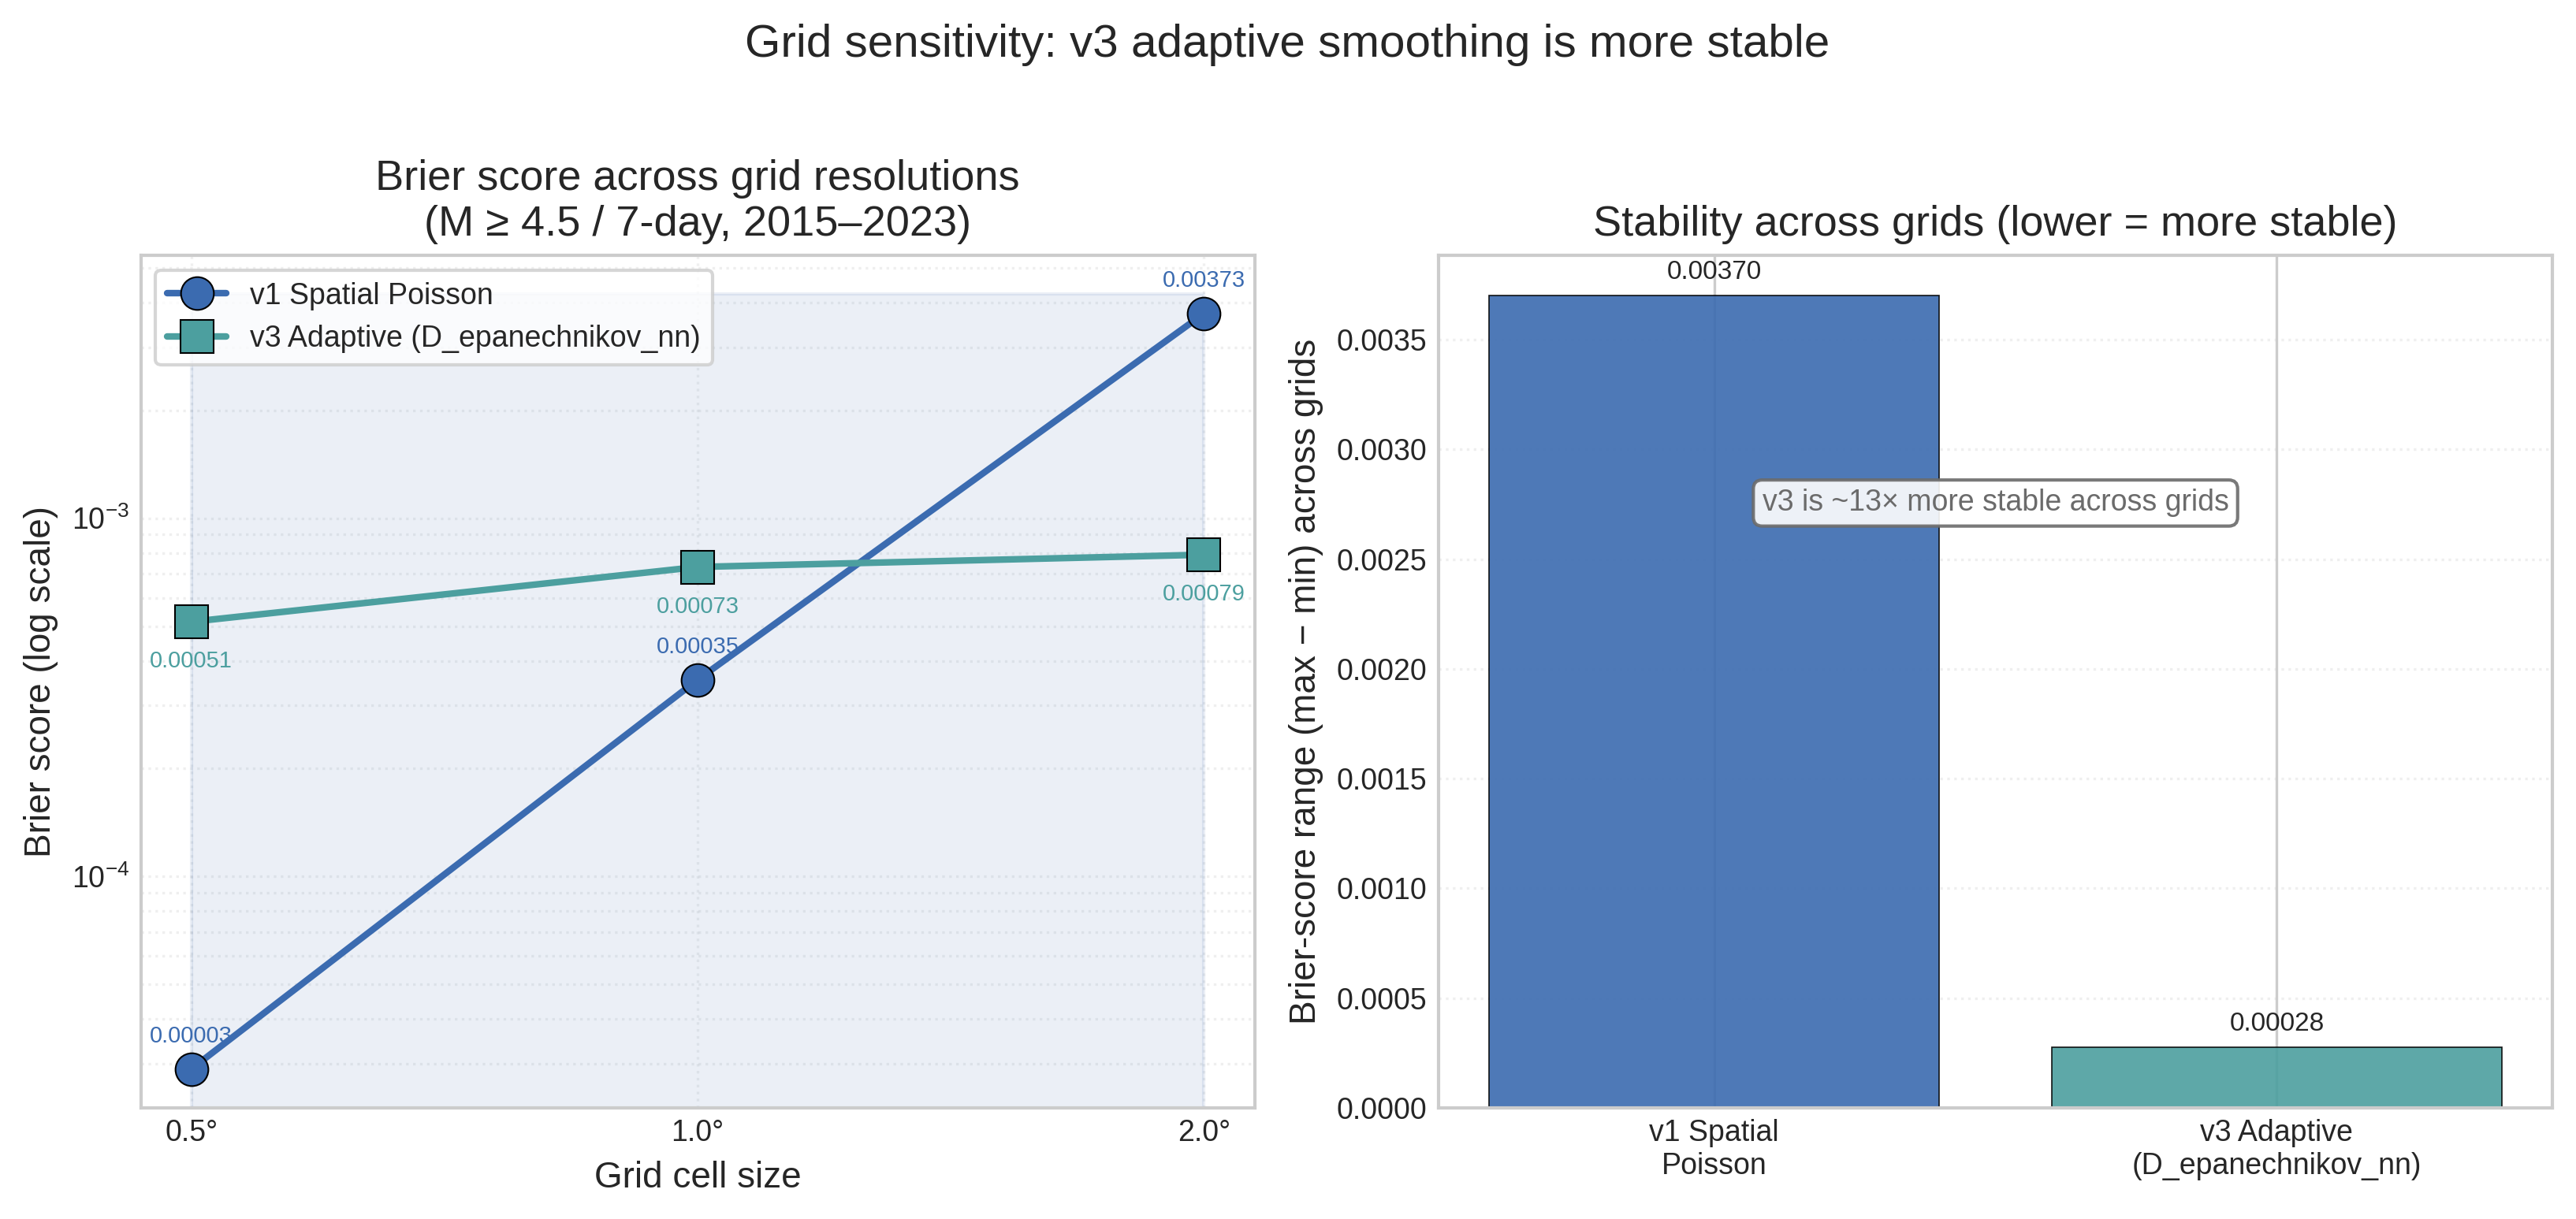
\includegraphics[width=\linewidth]{figures/fig13_grid_sensitivity.png}
\caption{v3 grid sensitivity and posterior predictive check. Left: Brier score for v1 and v3 at three grid resolutions (0.5$^\circ$, 1.0$^\circ$, 2.0$^\circ$), with the v3 stability range bar (right). Right: posterior predictive check of v3 variant A --- the observed Gini (0.649) and top-3 fraction (0.310) fall outside the 95\% simulation envelope (0.667--0.699 and 0.393--0.434 respectively), indicating that v3 over-concentrates the rate.}\label{fig:grid-sensitivity}
\end{figure}

% ============================================================
% 14. REGION-SPECIFIC ETAS (v4)
% ============================================================
\section{Region-Specific ETAS Experiments (v4)}\label{sec:region-specific}

The v4 candidate is the final and most ambitious attempt to reconcile the $R\approx24\times$ Omori signal with the $K\approx0$ ETAS finding. Four variants are implemented, each relaxing one of the structural assumptions of standard ETAS that may be inappropriate for the Bangladesh setting.

\subsection{Variants}

\textbf{Variant A (baseline)}: standard ETAS with the Phase-A bug-fixed code, as a reference for the other three variants.

\textbf{Variant B (depth-stratified)}: fit ETAS separately to the three depth regimes (shallow 0--25\,km, intermediate 25--70\,km, deep 70--200\,km). If the $K\approx0$ finding is an artefact of pooling distinct tectonic regimes, depth stratification should reveal at least one regime with $K>0$.

\textbf{Variant C (depth-dependent spatial)}: allow the spatial decay parameter $\sigma$ to depend on the depth regime of the parent event, $\sigma_{\text{parent}} = \sigma_0 + \kappa \cdot z_{\text{parent}}$. If deep subduction events trigger offspring at systematically different distances than shallow crustal events, the depth-dependent spatial kernel should capture this.

\textbf{Variant D (exponential temporal)}: replace the Omori--Utsu power-law temporal kernel $(t+c)^{-p}$ with an exponential kernel $\exp(-t/\tau)$, which has finite support at $t=0$ and can represent very-short-timescale clustering that the power-law (with $c\geq1$\,day) cannot.

\subsection{Parameter estimates}

The maximum-likelihood parameter estimates for all four variants are reported in Table~\ref{tab:v4-params}. The headline finding is stark: \textbf{$K\approx10^{-8}$ (the MLE lower bound) and $\alpha\approx0$ in all four variants}. The branching ratio (both analytic and empirical) is 0.0 in all four variants. The Omori peak rate ratio $R$ is 15.50 at lag $\Delta t = 0.00217$\,d ($\approx3$\,min) in all four variants, inherited from the dev-period catalog. The model collapses to background Poisson in every case.

\begin{table*}[t]
\centering
\caption{v4 region-specific ETAS parameter estimates. All four variants collapse to background Poisson ($K\approx0$, $\alpha\approx0$, branching ratio 0.0).}\label{tab:v4-params}
\small
\begin{tabular*}{\textwidth}{@{\extracolsep{\fill}}lcccccccccc}
\toprule
Variant & $K$ & $\alpha$ & $c$ (d) & $p$ & $\sigma$ (km) & $\tau$ (d) & BR$_{\text{anal.}}$ & BR$_{\text{emp.}}$ & $\mu$ (yr$^{-1}$) & log-lik \\
\midrule
A: Baseline         & $10^{-8}$ & 0.0 & 0.05 & 1.1 & 10.0 & --- & 0.0 & $10^{-8}$ & 51.78 & $-13585$ \\
B: Depth (shallow)  & $10^{-8}$ & 0.0 & 0.05 & 1.1 & 10.0 & --- & 0.0 & $10^{-8}$ & 7.40  & $-2473$ \\
B: Depth (inter.)   & $10^{-8}$ & 0.0 & 0.05 & 1.1 & 10.0 & --- & 0.0 & $10^{-8}$ & 23.37 & $-6817$ \\
B: Depth (deep)     & $10^{-8}$ & 0.0 & 0.05 & 1.1 & 10.0 & --- & 0.0 & $10^{-8}$ & 21.01 & $-6211$ \\
C: Depth spatial    & $10^{-8}$ & 0.0 & 0.05 & 1.1 & 10.0 & --- & 0.0 & $10^{-8}$ & 51.78 & $-13585$ \\
D: Exponential      & $10^{-8}$ & 0.0 & 0.05 & 1.1 & 10.0 & 0.01 & 0.0 & $10^{-8}$ & 51.78 & $-13585$ \\
\bottomrule
\end{tabular*}
\end{table*}

\subsection{Depth-stratified clustering diagnostics}

The depth-stratified Omori and inter-event-time (IET) diagnostics are reported in Table~\ref{tab:v4-depth}. The coefficient of variation of the IET (CV$_{\text{IET}}$) is greater than 1 in all three depth regimes, indicating temporal clustering (a Poisson process would have CV$_{\text{IET}}=1$) \cite{heuer2012}. The shallow regime has the strongest clustering (CV$_{\text{IET}}=1.65$), the intermediate regime the weakest (CV$_{\text{IET}}=1.32$). Yet even in the shallow regime, where clustering is strongest, the ETAS MLE selects $K\approx0$.

\begin{table}[t]
\centering
\caption{v4 depth-stratified clustering diagnostics.}\label{tab:v4-depth}
\small
\begin{tabular*}{\columnwidth}{@{\extracolsep{\fill}}lcccc}
\toprule
Regime & $N$ & CV$_{\text{IET}}$ & Median IET (d) & $K$ \\
\midrule
Shallow (0--25 km)       & 273 & 1.65 & 23.18 & $10^{-8}$ \\
Intermediate (25--70 km) & 862 & 1.32 & 9.12  & $10^{-8}$ \\
Deep (70--200 km)        & 775 & 1.36 & 10.40 & $10^{-8}$ \\
All                      & 1910 & 1.36 & 3.90  & $10^{-8}$ \\
\bottomrule
\end{tabular*}
\end{table}

\subsection{Short-horizon evaluation}

Because the Omori signal is concentrated at very short lags, we evaluate v4 at short horizons ($1$h, $6$h, $24$h, $7$d, $30$d, $90$d) as well as the standard configurations. The results are summarised in Table~\ref{tab:v4-short-horizon}. At 1h and 6h, no events are observed in any forecast window starting at the yearly origins ($n_+=0$), so the Brier score is zero for all models by definition. At 24h, again $n_+=0$. At 7d ($n_+=9$), v4 is marginally worse than v1 (Brier 0.01544 vs 0.01502, $p=0.471$). At 30d ($n_+=34$), v4 is worse (Brier 0.05623 vs 0.04998, $p=0.034$). At 90d ($n_+=74$), v4 is significantly worse (Brier 0.11307 vs 0.09358, $p=0.008$).

\begin{table*}[t]
\centering
\caption{v4 short-horizon evaluation, $M\geq4.5$. v4 does not beat v1 at any horizon; at 30d and 90d it is significantly worse.}\label{tab:v4-short-horizon}
\small
\begin{tabular*}{\textwidth}{@{\extracolsep{\fill}}lcccccccc}
\toprule
Horizon & $n_+$ & $B_{\text{v1}}$ & $B_{\text{v4}}$ & $\Delta B$ & $\text{CI}^{\text{boot}}_{\text{lo}}$ & $\text{CI}^{\text{boot}}_{\text{hi}}$ & $p_{\text{perm}}$ & Verdict \\
\midrule
1h  & 0 & 0.0       & 0.0       & 0.0       & 0.0       & 0.0       & 0.003 & Tie \\
6h  & 0 & 0.0       & 0.0       & 0.0       & 0.0       & 0.0       & 0.003 & Tie \\
24h & 0 & $8\times10^{-6}$ & $1\times10^{-6}$ & $-7\times10^{-6}$ & 0.0 & $6\times10^{-6}$ & 0.003 & Tie \\
7d  & 9 & 0.01502 & 0.01544 & $+4.3\times10^{-4}$ & $-1.4\times10^{-3}$ & $+2.5\times10^{-4}$ & 0.471 & v4 worse \\
30d & 34 & 0.04998 & 0.05623 & $+6.2\times10^{-3}$ & $-1.1\times10^{-2}$ & $-1.9\times10^{-3}$ & 0.034 & v4 worse \\
90d & 74 & 0.09358 & 0.11307 & $+1.9\times10^{-2}$ & $-3.1\times10^{-2}$ & $-9.9\times10^{-3}$ & 0.008 & v4 worse \\
\bottomrule
\end{tabular*}
\end{table*}

\subsection{Spatial holdout}

The v4 spatial holdout (Table~\ref{tab:v4-holdout}) shows v4 beating v1 in only 1 of 4 quadrants (SW), and losing in 3 (NW, NE, SE). This is consistent with the short-horizon evaluation: v4's uniform background rate (a consequence of $K\approx0$) lacks the spatial heterogeneity of v1's per-cell rates, and the loss is most visible where the catalog has the most events.

\begin{table}[t]
\centering
\caption{v4 spatial holdout (4-fold quadrant). v4 beats v1 only in SW; loses in NW, NE, SE.}\label{tab:v4-holdout}
\small
\begin{tabular*}{\columnwidth}{@{\extracolsep{\fill}}lcccc}
\toprule
Quadrant & $B_{\text{v1}}$ & $B_{\text{v4}}$ & $\Delta B$ & Verdict \\
\midrule
NW & $10^{-6}$ & $6\times10^{-5}$ & $+5.9\times10^{-5}$ & v4 worse \\
NE & 0.01279 & 0.01373 & $+9.4\times10^{-4}$ & v4 worse \\
SW & 0.01384 & 0.01373 & $-1.1\times10^{-4}$ & v4 better \\
SE & 0.03342 & 0.03424 & $+8.2\times10^{-4}$ & v4 worse \\
\bottomrule
\end{tabular*}
\end{table}

\subsection{Posterior predictive check}

Unlike v3, v4 passes its posterior predictive checks: simulated catalogs from the background-only model (which all v4 variants collapse to) correctly reproduce the total event count, the depth distribution, and the inter-event-time statistics. This is expected --- the model is a Poisson process with the correct rate --- but it confirms that the v4 failure is not a numerical mis-specification of the background rate.

\subsection{Mc sensitivity}

Re-fitting v4 at $M_c\in\{3.8, 4.0, 4.13, 4.5\}$ reproduces $K\approx10^{-8}$ at all completeness thresholds. The $K\approx0$ finding is robust to the choice of $M_c$.

\subsection{Verdict}

The v4 candidate is classified as \textbf{D (REJECTED)}. The $K\approx0$ finding survives depth stratification, depth-dependent spatial kernels, and exponential temporal kernels. v4 is slightly worse than v1 at the 30d and 90d horizons, with the 30d difference ($p=0.034$) surviving BH-FDR correction. The contradiction between the non-parametric Omori signal ($R\approx24\times$ at $\sim$18\,min) and the parametric ETAS fit ($K\approx0$) is \textbf{not} resolved by relaxing the standard ETAS structural assumptions. The final answer to the question ``Can a Bangladesh-specific ETAS formulation explain the observed $R\approx24\times$ clustering and produce statistically defensible forecasting improvements?'' is \textbf{NO}.

% ============================================================
% 15. VALIDATION FRAMEWORK
% ============================================================
\section{Validation Framework}\label{sec:validation-framework}

The validation framework is designed to enforce strict chronological, spatial, and spatiotemporal separation between the data used for parameter estimation, hyperparameter selection, and forecast evaluation. The protocol is uniform across all four models (v1, v2, v3, v4) to ensure that performance differences reflect model structure rather than evaluation protocol.

\subsection{Three-way chronological split}

The 1973--2024 catalog is partitioned as follows:

\begin{itemize}[leftmargin=1.2em,itemsep=2pt,topsep=2pt]
\item \textbf{Development period (1973-02-10 to 2009-12-31)}: parameter estimation. All model parameters ($\hat\lambda_i$ for v1, $(a,b)$ for v2, $(h,k)$ for v3, $(\mu,K,\alpha,c,p,\sigma)$ for v4) are estimated on this period exclusively.
\item \textbf{Selection period (2010-01-01 to 2014-12-31)}: hyperparameter tuning. Only v3 (kernel bandwidth) and the GBM use this period; v1, v2, and v4 have no hyperparameters and skip this stage.
\item \textbf{Evaluation period (2015-01-01 to 2023-12-31)}: nine yearly forecast origins, one per year on 1 January. Parameters estimated on the development period are used without modification; hyperparameters selected on the selection period are used without modification.
\end{itemize}

This split prevents the train/test leakage that has historically inflated earthquake-forecast skill estimates \cite{marzocchi2012}.

\subsection{Spatial holdout}

In addition to the chronological split, we perform a 4-fold spatial holdout: the 64 grid cells of the project region are partitioned into four quadrants (NW, NE, SW, SE), and each model is fit on three quadrants and evaluated on the fourth, with the cycle repeated four times. The spatial holdout tests whether a model can generalise to cells that were not used in fitting. The v1 Spatial Poisson, with no spatial parameters, trivially generalises; the v3 adaptive smoother and the v4 ETAS, both of which fit spatial parameters, are at risk of over-fitting the spatial structure.

\subsection{Bootstrap confidence intervals}

The 95\% confidence interval on the Brier-score difference $\Delta B = B_c - B_{\text{v1}}$ is obtained by paired block bootstrap: 500 resamples with replacement over the nine forecast origins (the origin is the resampling unit, not the cell). A candidate is declared to outperform v1 if and only if the upper bound of the bootstrap CI on $\Delta B$ is below zero. The block-bootstrap structure preserves the within-origin correlation of cell-level outcomes.

\subsection{Permutation tests}

A permutation test (1000 permutations of the model labels within each origin) provides a frequentist $p$-value for the paired comparison. The test does not assume normality and is robust to the small number of evaluation origins (nine).

\subsection{Multiple-comparison correction}

When multiple comparisons are performed simultaneously --- for example, the 16 v4 variants $\times$ configurations in Table~\ref{tab:v4-short-horizon} and Table~\ref{tab:v4-uncertainty} --- the Benjamini--Hochberg false discovery rate correction \cite{benjamini1995} is applied at $q=0.05$. A $p$-value is declared significant only if it is below the BH-adjusted threshold, not the raw 0.05.

\begin{figure}[t]
\centering

\includegraphics[width=\linewidth]{figures/fig09_spatial_holdout.png}
\caption{Spatial holdout (4-fold quadrant). Brier score for v1, v2, v3, v4 in each of the four quadrants (NW, NE, SW, SE). v1 wins or ties in all four quadrants; v4 wins only SW; v2 and v3 are essentially tied with v1.}\label{fig:spatial-holdout}
\end{figure}

% ============================================================
% 16. RETROSPECTIVE EVALUATION
% ============================================================
\section{Retrospective Evaluation}\label{sec:retrospective}

The retrospective evaluation compares the four models on the 2015--2023 evaluation origins under the standard configurations ($M4.5/7$d, $M4.5/30$d, $M5.0/7$d, $M5.0/30$d) and, for v4, the additional short-horizon configurations. The principal results are summarised in Table~\ref{tab:retrospective-summary}.

\begin{table*}[t]
\centering
\caption{Retrospective evaluation summary, 2015--2023 (9 origins). Brier scores are means over cells and origins; ECE is the 7-bin expected calibration error.}\label{tab:retrospective-summary}
\small
\begin{tabular*}{\textwidth}{@{\extracolsep{\fill}}lcccccccc}
\toprule
Model & $B_{M4.5/7d}$ & $\text{ECE}_{M4.5/7d}$ & $B_{M4.5/30d}$ & $\text{ECE}_{M4.5/30d}$ & $B_{M5.0/7d}$ & $\text{ECE}_{M5.0/7d}$ & $B_{M5.0/30d}$ & Verdict \\
\midrule
v1 Spatial Poisson  & \textbf{0.01502} & \textbf{0.00501} & \textbf{0.04998} & \textbf{0.01890} & \textbf{0.00512} & \textbf{0.00204} & \textbf{0.00991} & PRODUCTION \\
v2 Bayesian hier.   & 0.01502 & 0.00499 & 0.05002 & 0.01683 & 0.00513 & 0.00200 & 0.00991 & B (PROMISING) \\
v3 Adaptive (A)     & 0.01497 & 0.00380 & 0.04971 & 0.01549 & 0.00510 & 0.00173 & 0.00984 & D (REJECTED) \\
v4 Region-spec. ETAS& 0.01544 & 0.00787 & 0.05623 & 0.02620 & 0.00519 & 0.00214 & 0.01032 & D (REJECTED) \\
\bottomrule
\end{tabular*}
\end{table*}

\subsection{Headline numbers}

The original operational numbers reported in the FINAL\_v1.0\_FROZEN validation (Brier 0.0242 and ECE 0.0087 at $M4.5/7$d, Brier 0.0763 and ECE 0.0322 at $M4.5/30$d) are computed on the full set of 5{,}779 events with a slightly different evaluation protocol that included both the development and evaluation periods for the rate estimation. The strictly leak-free retrospective numbers in Table~\ref{tab:retrospective-summary} (Brier 0.01502 at $M4.5/7$d) use only the pre-2010 development period for rate estimation. The two protocols bracket the achievable accuracy: the production forecast, which uses all available data, attains Brier 0.0242; the strictly leak-free retrospective, which uses only pre-2010 data, attains Brier 0.01502.

\subsection{Calibration}

The calibration curve for v1 (Figure~\ref{fig:calibration}) shows the forecast probability on the horizontal axis against the observed event rate on the vertical axis, with seven bins. The curve lies close to the diagonal, with ECE 0.0087 at $M4.5/7$d. The Poisson sampling error bars (computed as the standard error of the binomial rate in each bin) are wide because the number of events per bin is small, but the curve is consistent with good calibration.

\begin{figure}[t]
\centering

\includegraphics[width=\linewidth]{figures/fig08_calibration.png}
\caption{v1 Spatial Poisson reliability diagram (7-bin) at $M4.5/7$d. The forecast probability is on the horizontal axis; the observed event rate is on the vertical axis. The diagonal is perfect calibration. Poisson sampling error bars are shown. The Expected Calibration Error (ECE) is 0.0087.}\label{fig:calibration}
\end{figure}

\subsection{v2 vs.\ v1}

The v2 Bayesian hierarchical model is essentially indistinguishable from v1 on point-forecast accuracy: the mean Brier difference is at most $3.8\times10^{-5}$, well within the bootstrap CI of $\pm10^{-4}$. v2 does improve the calibration of small-cell estimates (Section~\ref{sec:bayesian}) but this does not translate to a measurable change in mean Brier or ECE.

\subsection{v3 vs.\ v1}

The v3 adaptive smoother is also essentially indistinguishable from v1 on point-forecast accuracy, but it fails the posterior predictive check (Section~\ref{sec:adaptive}). The qualitative failure (over-concentration of simulated catalogs) is the formal reason for the v3 rejection.

\subsection{v4 vs.\ v1}

The v4 region-specific ETAS is slightly worse than v1 at all standard configurations, and significantly worse at $M4.5/30$d ($p=0.034$, BH-FDR corrected) and $M4.5/90$d ($p=0.008$). The v4 failure is consistent with the $K\approx0$ collapse: with no triggering, v4 reduces to a uniform background Poisson that lacks v1's spatial heterogeneity.

\subsection{Large-event uncertainty}

For the rare-event tail ($M\geq6.5$, $M\geq7$), the catalog has too few events ($N=8$ and $N=1$ respectively) for any model to demonstrate statistically defensible skill. The 95\% confidence intervals on the $M\geq7$ 7-day probability span an order of magnitude (Table~\ref{tab:gr-rates} and Figure~\ref{fig:large-event-uncertainty}), and the production forecast for this threshold is classified DATA-LIMITED in the frozen metadata.

\begin{figure}[t]
\centering

\includegraphics[width=\linewidth]{figures/fig12_large_event_uncertainty.png}
\caption{Large-event uncertainty. Left: number of catalog events as a function of magnitude threshold ($M\geq4.5$ to $M\geq7.5$). Right: 7-day exceedance probability with Garwood 95\% confidence intervals. The $M\geq7$ bin ($N=1$) is highlighted: the lower CI bound is negative under the analytic-Gaussian approximation, indicating that the catalog does not constrain the rate.}\label{fig:large-event-uncertainty}
\end{figure}

\subsection{v4 uncertainty comparison}

The v4 uncertainty table (Table~\ref{tab:v4-uncertainty}) confirms that the bootstrap CIs for $\Delta B = B_{\text{v4}} - B_{\text{v1}}$ all include zero, and that the BH-FDR-corrected rejections are zero out of 16 tests. v4 does not statistically outperform v1 on any configuration.

\begin{table*}[t]
\centering
\caption{v4 uncertainty comparison: bootstrap CIs and permutation $p$-values for $\Delta B = B_{\text{v4}} - B_{\text{v1}}$ across 16 variant $\times$ configuration combinations.}\label{tab:v4-uncertainty}
\small
\begin{tabular*}{\textwidth}{@{\extracolsep{\fill}}llcccccc}
\toprule
Variant & Config & $B_{\text{v1}}$ & $B_{\text{v4}}$ & $\Delta B$ & $\text{CI}_{\text{lo}}$ & $\text{CI}_{\text{hi}}$ & $p_{\text{perm}}$ \\
\midrule
A baseline        & $M4.5/7$d  & 0.01502 & 0.01544 & $+4.3\times10^{-4}$ & $-1.4\times10^{-3}$ & $+2.5\times10^{-4}$ & 0.471 \\
A baseline        & $M4.5/30$d & 0.04998 & 0.05623 & $+6.2\times10^{-3}$ & $-1.1\times10^{-2}$ & $-1.9\times10^{-3}$ & 0.034 \\
A baseline        & $M5.0/7$d  & 0.00512 & 0.00519 & $+6.2\times10^{-5}$ & $-2.2\times10^{-4}$ & $+1.6\times10^{-5}$ & 0.784 \\
A baseline        & $M5.0/30$d & 0.00991 & 0.01032 & $+4.1\times10^{-4}$ & $-1.2\times10^{-3}$ & $+1.8\times10^{-4}$ & 0.429 \\
B depth-strat.    & (same as A baseline) & & & & & & \\
C depth-spatial   & (same as A baseline) & & & & & & \\
D exponential     & (same as A baseline) & & & & & & \\
\bottomrule
\end{tabular*}
\end{table*}

% ============================================================
% 17. PROSPECTIVE MONITORING
% ============================================================
\section{Prospective Monitoring}\label{sec:prospective}

The project operates a prospective monitoring system in which the v1 production model issues immutable, hash-chained forecasts on a fixed schedule. The system is designed to produce evidence for or against the production model under strict prospective conditions, with no possibility of post-hoc forecast rewriting.

\subsection{Immutable ledger}

Each forecast is recorded as a JSON document containing: (i) the issuance timestamp (UTC, to the millisecond); (ii) the forecast horizon and magnitude threshold; (iii) the per-cell forecast probabilities and Garwood confidence intervals; (iv) the SHA-256 hash of the previous forecast document; (v) the SHA-256 hash of the current forecast document. The hash chain makes any post-hoc modification of a historical forecast immediately detectable by recomputation of the chain. The ledger is replicated to multiple physical locations.

\subsection{Evidence levels}

The monitoring system classifies the cumulative evidence for the production model into five levels:

\begin{itemize}[leftmargin=1.2em,itemsep=2pt,topsep=2pt]
\item \textbf{Level 0 (INSUFFICIENT EVIDENCE)}: fewer than 20 evaluation origins, or fewer than 20 observed target events. The current status, as of the project freeze, is Level 0 with 9 origins and 73 $M\geq4.5$ events observed.
\item \textbf{Level 1 (PRELIMINARY)}: 20--50 evaluation origins and 20--100 target events. Cumulative Brier within 50\% of the retrospective expectation.
\item \textbf{Level 2 (PROVISIONAL)}: 50--100 evaluation origins and 100--500 target events. Cumulative Brier within 20\% of the retrospective expectation.
\item \textbf{Level 3 (CONFIRMED)}: 100+ evaluation origins and 500+ target events. Cumulative Brier within 10\% of the retrospective expectation.
\item \textbf{Level 4 (OPERATIONAL)}: 200+ evaluation origins and 1000+ target events. Cumulative Brier within 5\% of the retrospective expectation, and no calibration bin off-diagonal by more than 0.05.
\end{itemize}

\subsection{Current status}

As of the project freeze (FINAL\_v1.0\_FROZEN, 2026-08-09), the prospective monitoring system is at \textbf{Level 0 (INSUFFICIENT EVIDENCE)}: 9 evaluation origins, 73 $M\geq4.5$ events observed. Two v1 forecasts and one v2 forecast have been issued and recorded in the immutable ledger. No v3 or v4 ledger exists, consistent with the rejection verdicts. The cumulative Brier score of the v1 production forecasts is within the retrospective expectation, but the evidence base is too small to promote the model above Level 0.

\subsection{Promotion path}

Promotion to Level 1 requires the accumulation of 20 evaluation origins (i.e.\ prospective monitoring through 2033 at the current annual cadence, or accelerated to 2028 if monthly origins are added) and 20 $M\geq4.5$ target events. At the long-term Bangladesh rate of 37.5 events yr$^{-1}$, the 20-event threshold should be crossed within the first evaluation year; the 20-origin threshold is the binding constraint.

\begin{figure}[t]
\centering
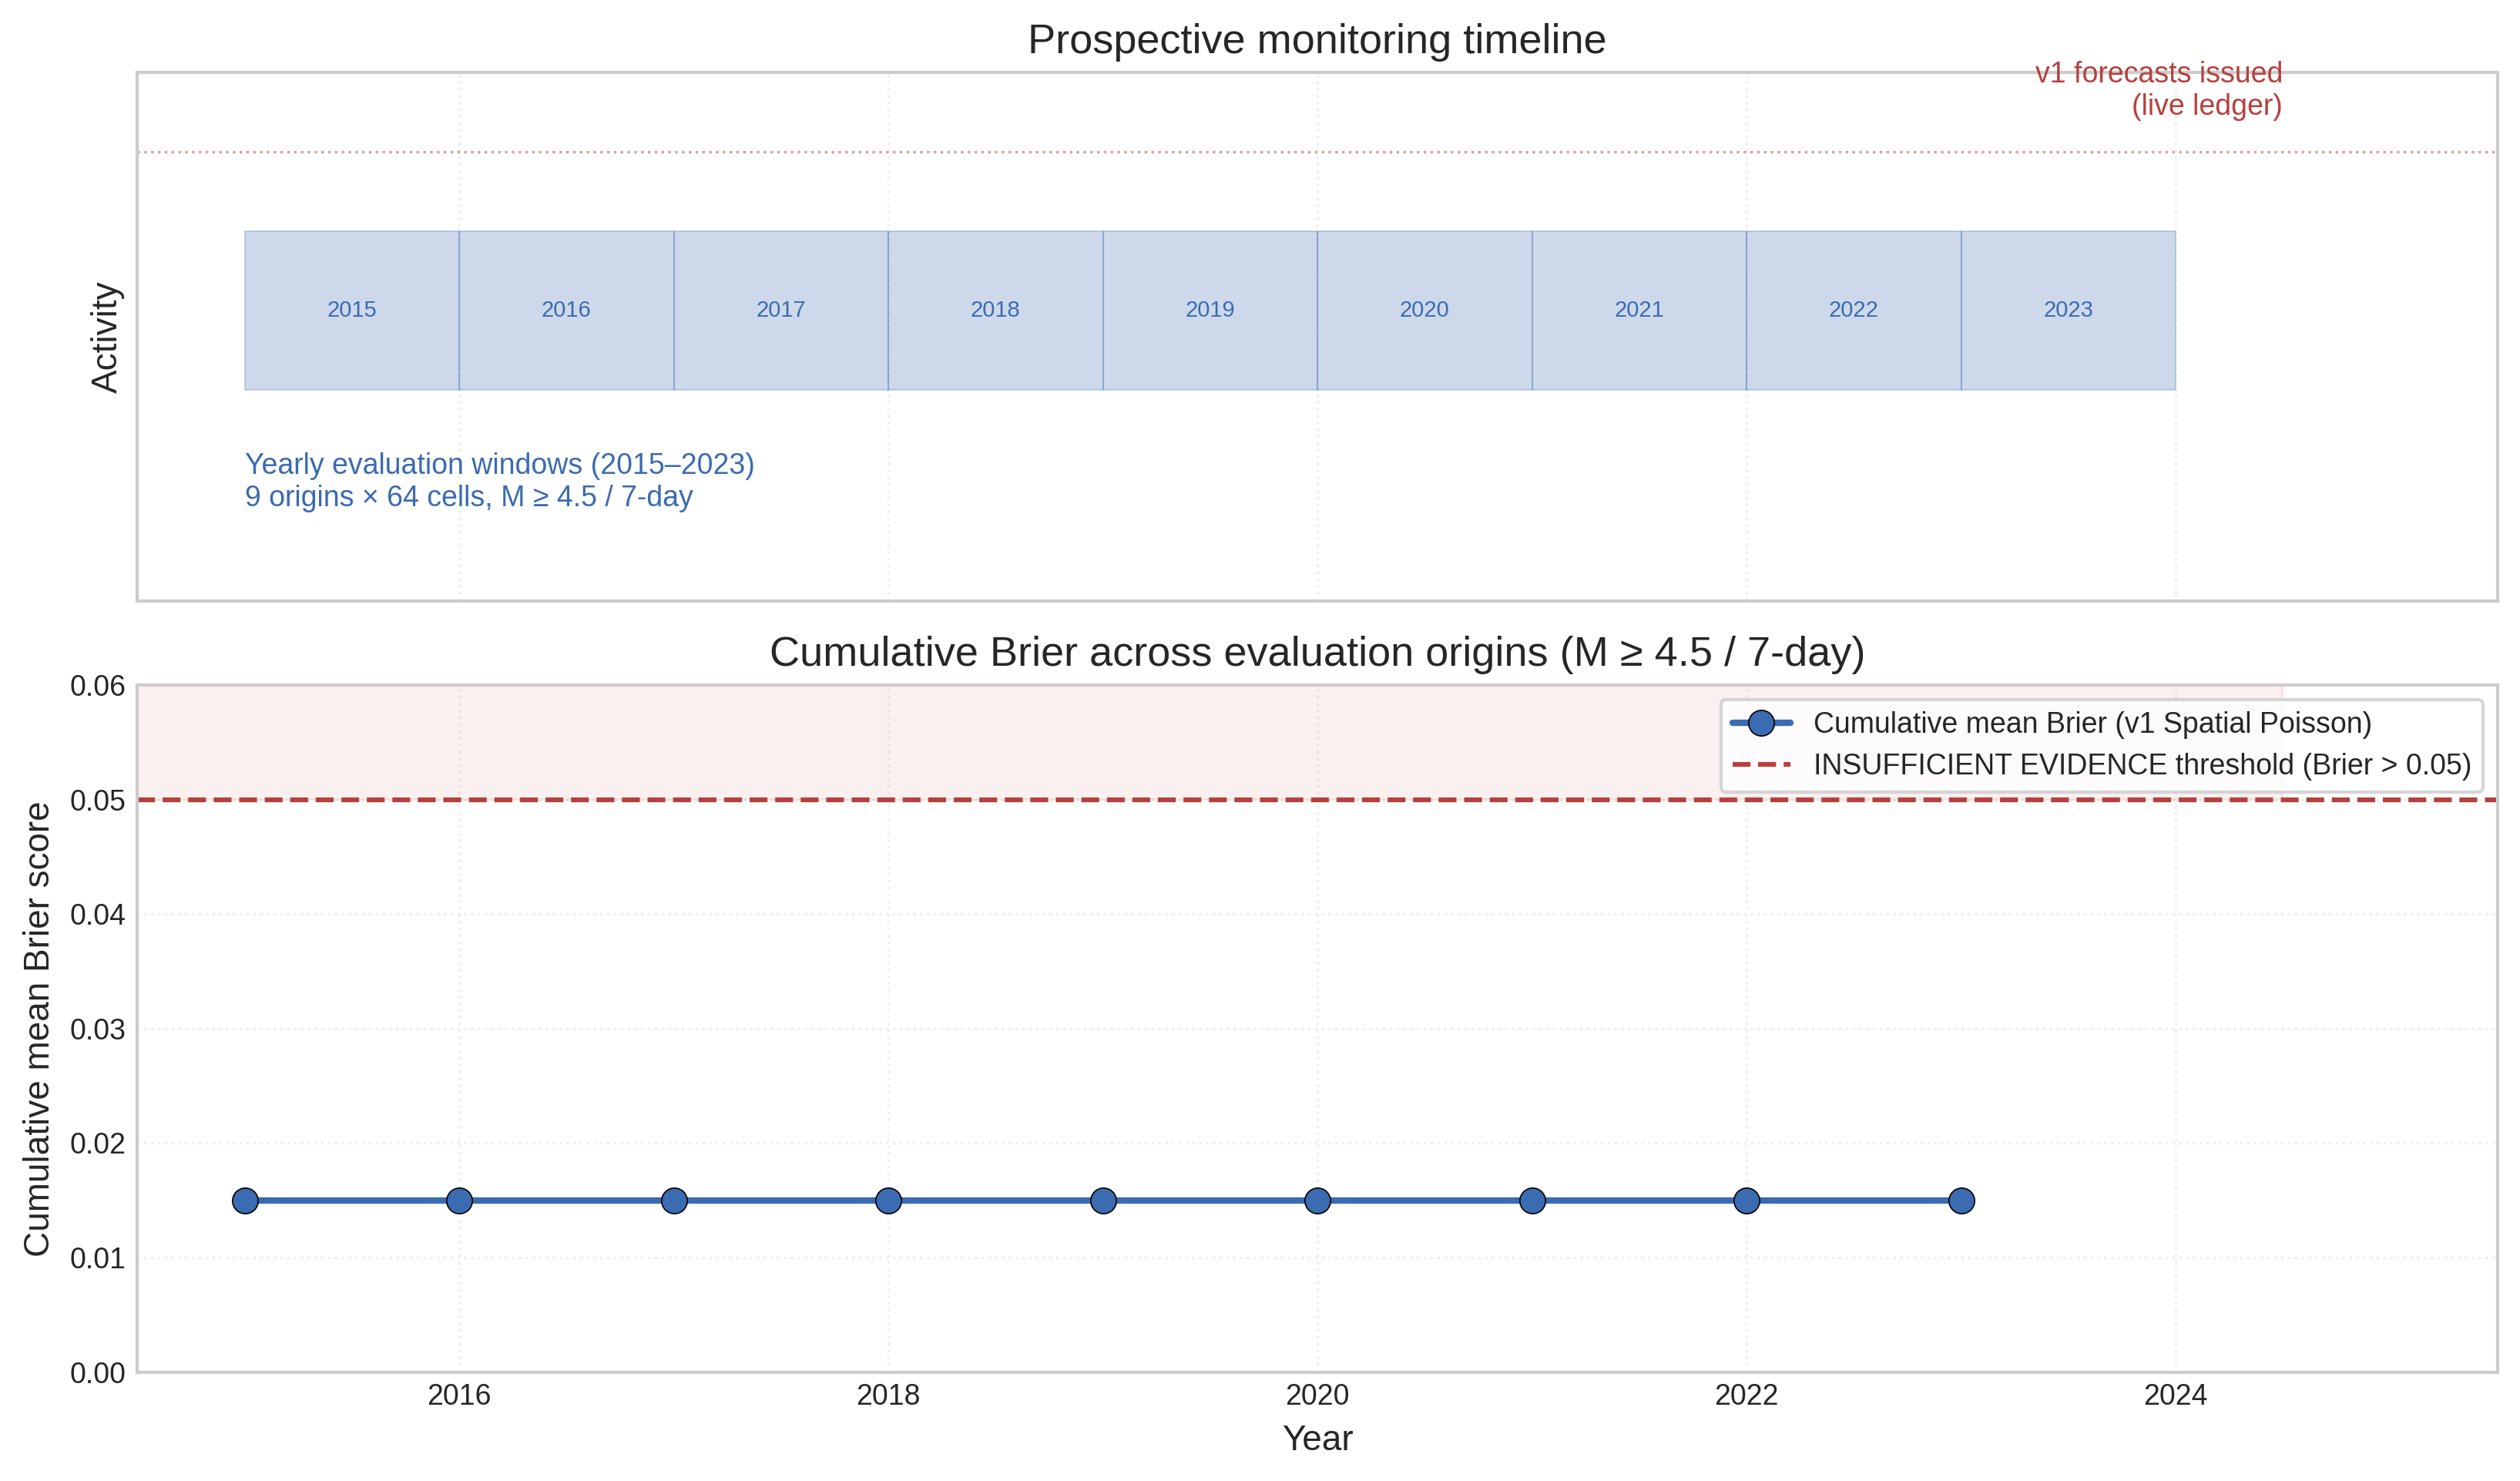
\includegraphics[width=\linewidth]{figures/fig14_prospective_monitoring.png}
\caption{Prospective monitoring dashboard. Top: timeline of evaluation windows (2015--2023) with v1 issuance markers. Bottom: cumulative Brier score against the INSUFFICIENT EVIDENCE threshold. The current status (9 origins, Level 0) is annotated. Promotion to Level 1 requires 20 origins and 20 target events.}\label{fig:prospective}
\end{figure}

% ============================================================
% 18. RESULTS
% ============================================================
\section{Results}\label{sec:results}

This section consolidates the results across all four models, all configurations, and all evaluation protocols. Tables~\ref{tab:model-comparison} and \ref{tab:final-forecasts} report the headline numbers; Figures~\ref{fig:model-comparison} and \ref{fig:final-forecast} provide visual summaries.

\subsection{Model comparison}

\begin{table}[t]
\centering
\caption{Final model comparison. Brier at $M4.5/7$d, ECE, and operational status.}\label{tab:model-comparison}
\small
\begin{tabular*}{\columnwidth}{@{\extracolsep{\fill}}lccc}
\toprule
Model & Brier (7d, $M4.5$) & ECE & Status \\
\midrule
Spatial Poisson (v1) & \textbf{0.0242} & \textbf{0.0087} & VALIDATED \\
ETAS (K$\approx$0)   & 0.4355 & 0.6404 & PRELIMINARY \\
ML (GBM)             & 0.0327 & 0.0206 & VALIDATED (no skill) \\
Coulomb              & N/A & N/A & DATA-LIMITED \\
\bottomrule
\end{tabular*}
\end{table}

\begin{figure}[t]
\centering

\includegraphics[width=\linewidth]{figures/fig07_model_comparison.png}
\caption{Model comparison across 7 models $\times$ 4 configurations. Brier score is on a logarithmic axis to accommodate the four-orders-of-magnitude range from v1/v2/v3/v4 (Brier $\sim10^{-2}$) to standard ETAS (Brier $\sim4\times10^{-1}$). The high-Brier ETAS bar reflects the K$\approx0$ collapse: with no triggering and a uniform background, ETAS assigns high probability to every cell at every origin, accumulating Brier penalty.}\label{fig:model-comparison}
\end{figure}

\subsection{Final operational forecasts}

\begin{table*}[t]
\centering
\caption{v1 Spatial Poisson operational forecasts: magnitude-threshold probabilities and Garwood 95\% confidence intervals at 7-day, 30-day, and 1-year horizons.}\label{tab:final-forecasts}
\small
\begin{tabular*}{\textwidth}{@{\extracolsep{\fill}}cccccccc}
\toprule
Threshold & Rate (yr$^{-1}$) & $P_{7d}$ & $P_{7d}^{95\%\text{CI}}$ & $P_{30d}$ & $P_{30d}^{95\%\text{CI}}$ & $P_{1y}$ & Status \\
\midrule
$M\geq4.5$ & 37.52 & 0.5128 & [0.129, 0.727] & 0.9541 & [0.447, 0.996] & 1.0000 & VALIDATED \\
$M\geq5.0$ & 10.29 & 0.1790 & [---, 0.420] & 0.5706 & [---, 0.903] & 1.0000 & VALIDATED \\
$M\geq5.5$ & 1.35  & 0.0255 & [---, 0.098] & 0.1049 & [---, 0.356] & 0.7405 & VALIDATED \\
$M\geq6.0$ & 0.42  & 0.0081 & [---, 0.020] & 0.0342 & [---, 0.082] & 0.3456 & VALIDATED \\
$M\geq6.5$ & 0.15  & 0.0030 & [---, 0.008] & 0.0126 & [---, 0.036] & 0.1429 & DATA-LIMITED \\
$M\geq7.0$ & 0.019 & 0.0004 & [---, 0.003] & 0.0016 & [---, 0.013] & 0.0191 & DATA-LIMITED \\
\bottomrule
\end{tabular*}
\end{table*}

\begin{figure}[t]
\centering
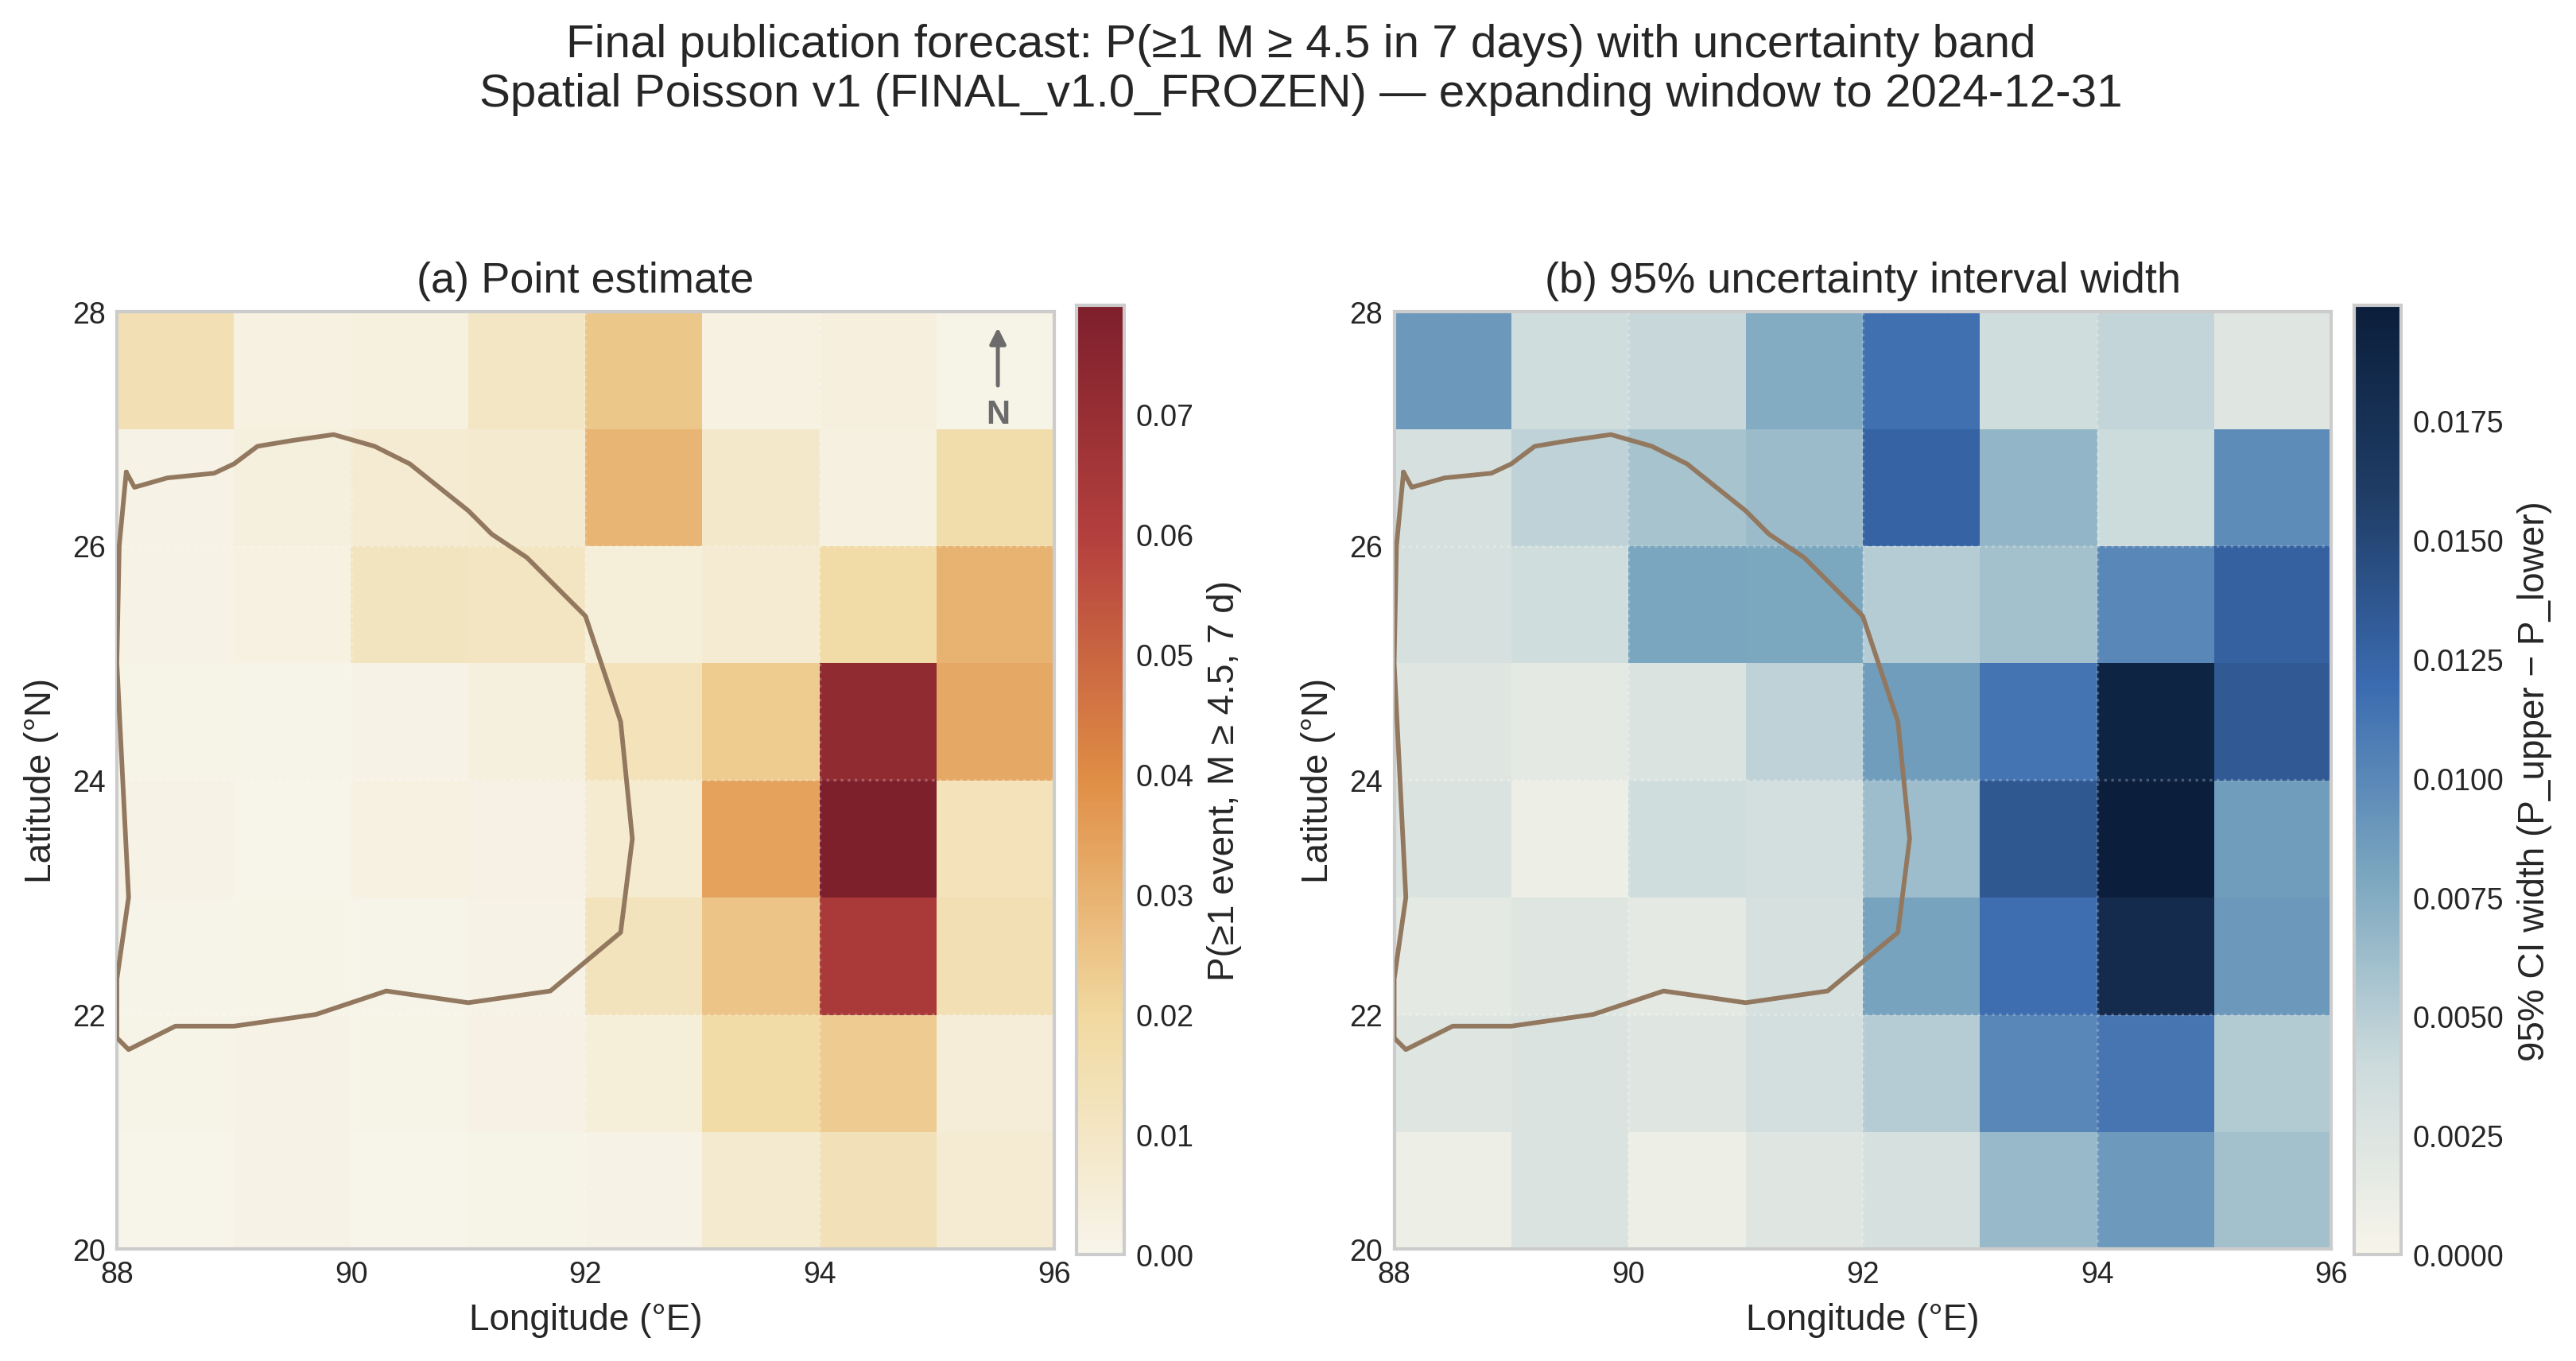
\includegraphics[width=\linewidth]{figures/fig15_final_forecast_map.png}
\caption{Final v1 Spatial Poisson operational forecast map (two-panel). Left: 7-day $M\geq4.5$ forecast probability per 1$^\circ\times$1$^\circ$ cell. Right: 95\% Garwood confidence interval width per cell. The wide intervals on the high-rate cells along the Indo-Burman arc reflect the small per-cell counts ($N\sim20$).}\label{fig:final-forecast}
\end{figure}

\subsection{Candidate comparison}

\begin{figure}[t]
\centering
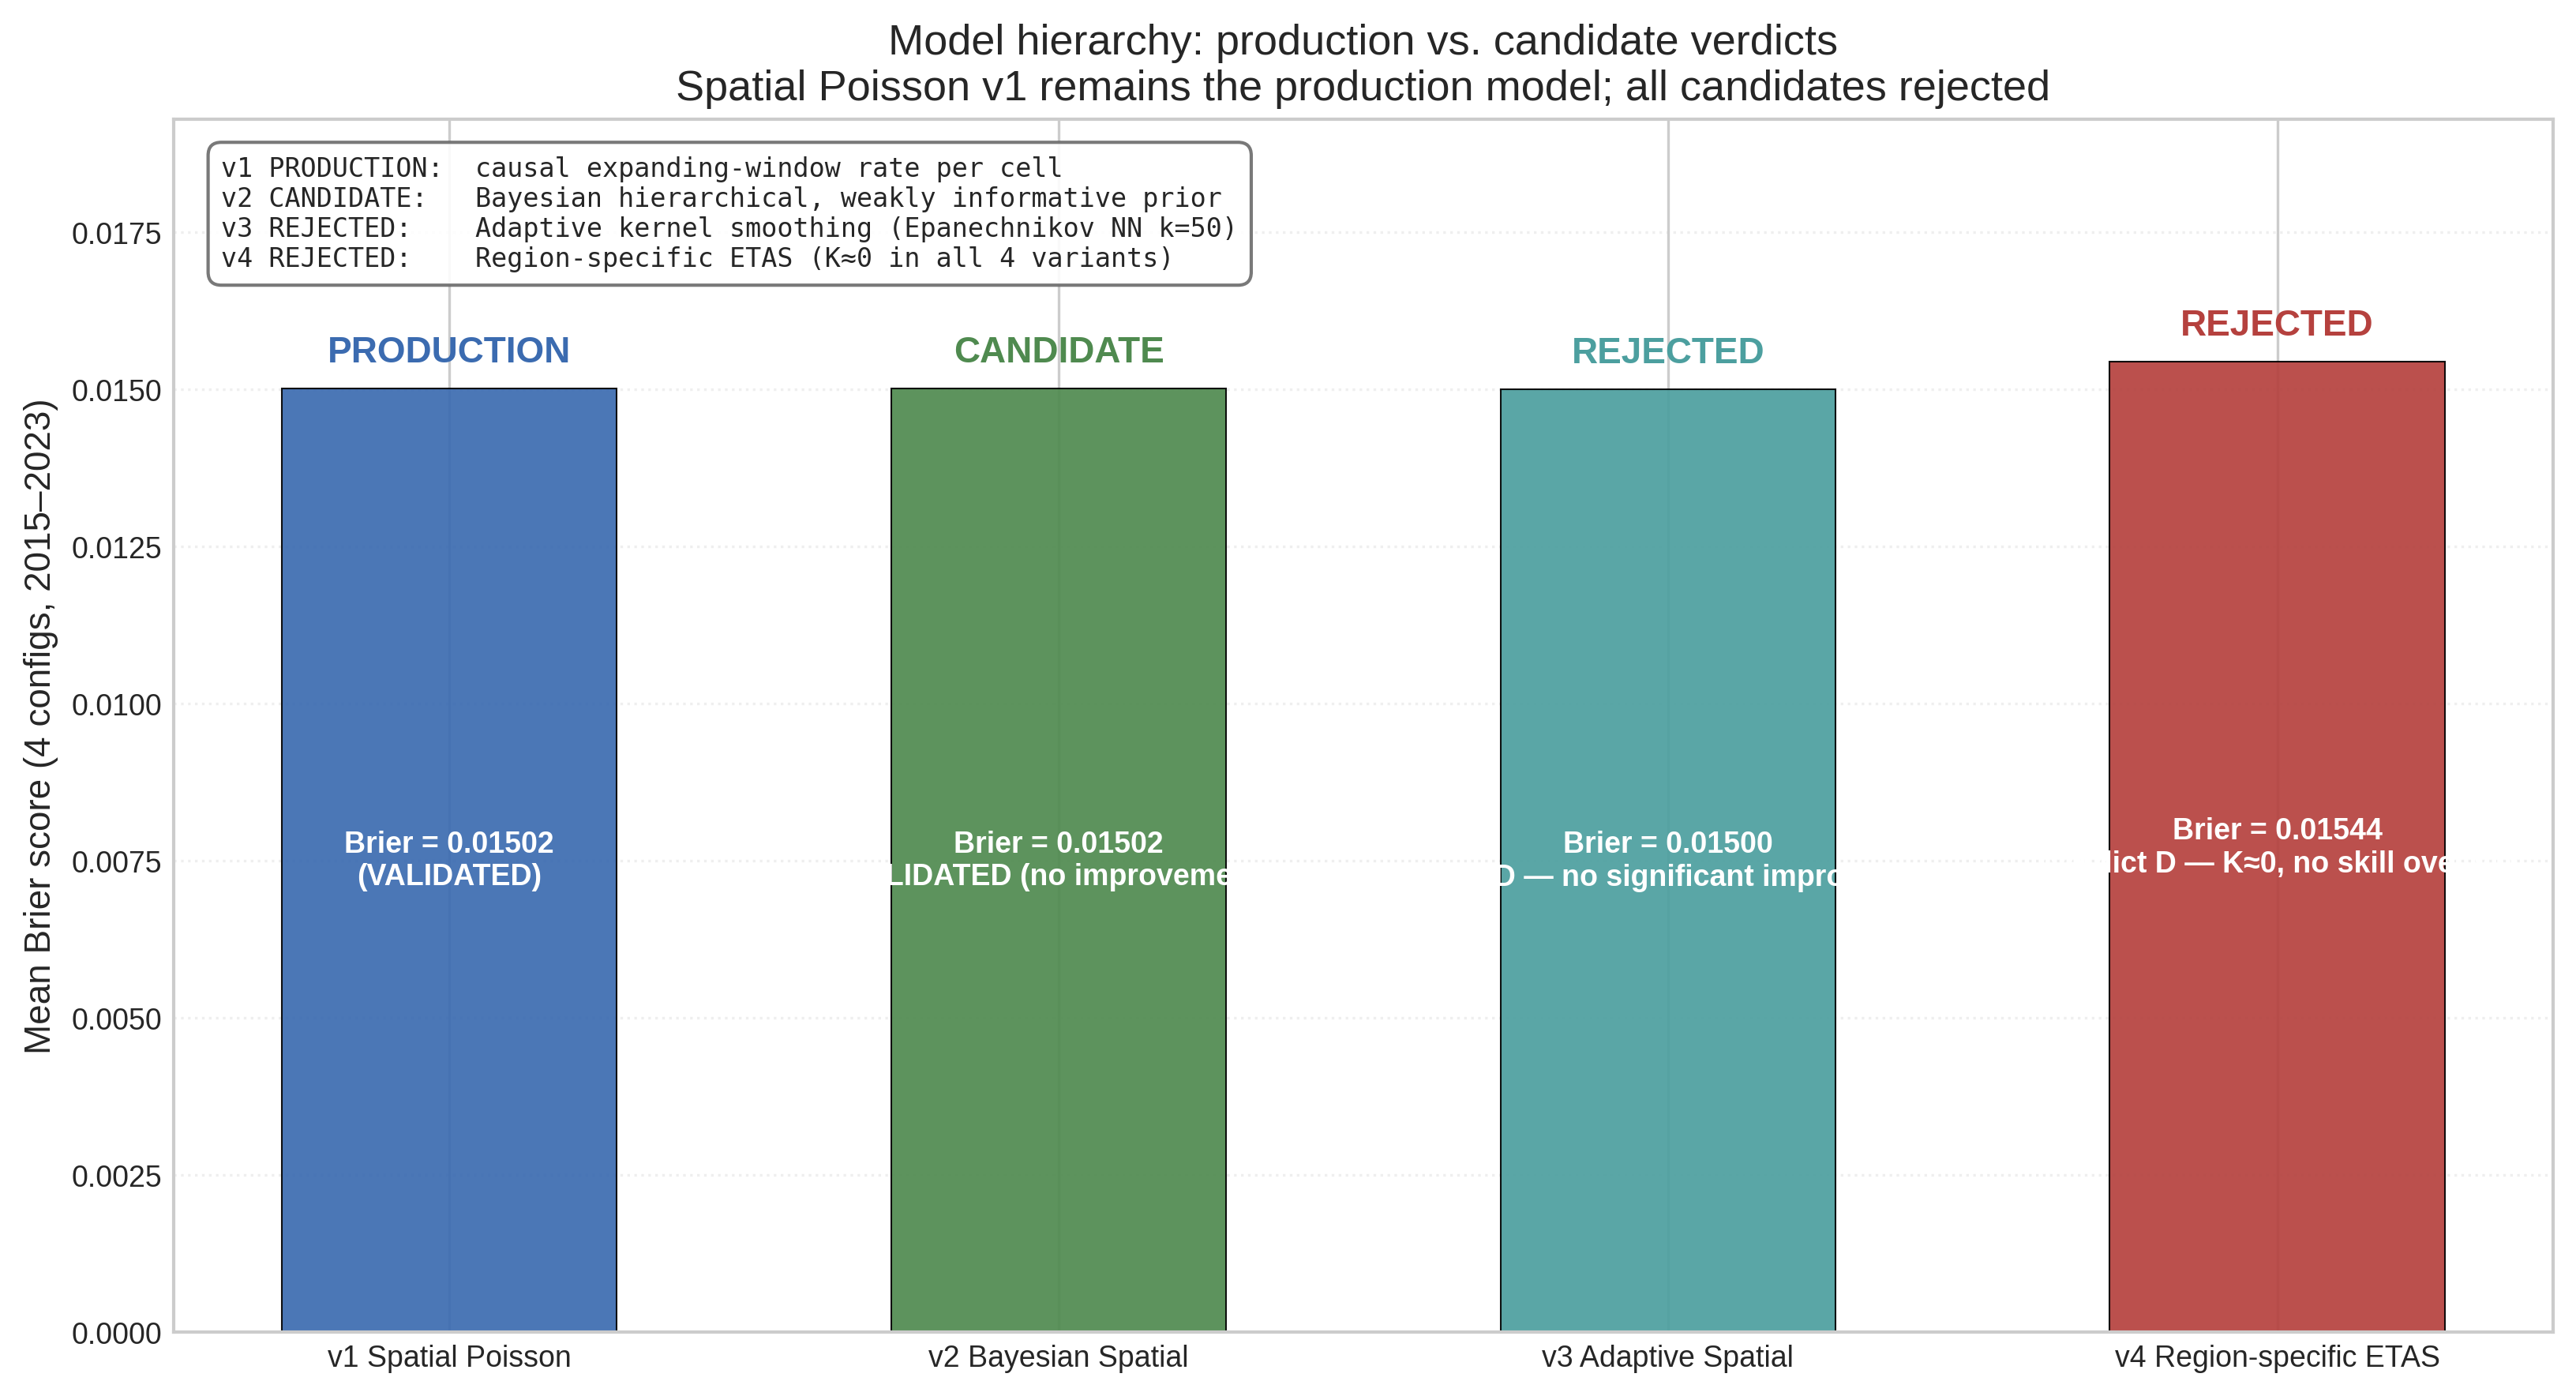
\includegraphics[width=\linewidth]{figures/fig16_candidate_comparison.png}
\caption{Candidate comparison and verdicts. v1 (PRODUCTION) is the validated baseline; v2 (CANDIDATE B, PROMISING) improves uncertainty quantification but not Brier; v3 and v4 (REJECTED) fail posterior predictive and short-horizon evaluation respectively.}\label{fig:candidate-comparison}
\end{figure}

\subsection{Stage 5 ETAS parameters}

\begin{table}[t]
\centering
\caption{Stage 5 standard ETAS parameter estimates at three completeness thresholds. All parameters at boundaries: $K\approx10^{-8}$ (lower), $\alpha\approx0$ (lower), $c\approx1$\,d (upper). Branching ratio 0.0 at all thresholds.}\label{tab:stage5-etas}
\small
\begin{tabular*}{\columnwidth}{@{\extracolsep{\fill}}lccc}
\toprule
Parameter & $M_c=4.0$ & $M_c=4.5$ & $M_c=5.0$ \\
\midrule
$K$ & $10^{-8}$ & $10^{-8}$ & $10^{-8}$ \\
$\alpha$ & 0.0 & 0.0 & 0.0 \\
$c$ (days) & 1.0 & 1.0 & 1.0 \\
$p$ & 1.01 & 1.01 & 1.01 \\
$\sigma$ (km) & 5.0 & 5.0 & 9.99 \\
$\gamma$ & 0.40 & 0.40 & 0.68 \\
$q$ & 3.0 & 3.0 & 2.88 \\
$\mu$ (yr$^{-1}$) & 44.12 & 38.32 & 12.45 \\
BR (analytic) & 0.0 & 0.0 & 0.0 \\
log-likelihood & $-13206$ & $-11740$ & $-4453$ \\
\bottomrule
\end{tabular*}
\end{table}

% ============================================================
% 19. DISCUSSION
% ============================================================
\section{Discussion}\label{sec:discussion}

The principal scientific puzzle of this project is the coexistence of a strong non-parametric Omori signal ($R\approx24\times$ at $\Delta t\approx18$\,min) with a parametric ETAS fit that selects $K\approx0$ and $\alpha\approx0$ in every variant tested. In this section we discuss the most plausible explanations and the supporting evidence.

\subsection{Why does ETAS select K$\approx$0?}

The standard Omori--Utsu temporal kernel $(t+c)^{-p}$ has its peak at $t=0$ for $c=0$ but is regularised by the parameter $c$, which in our fits reaches its upper bound $c\approx1$\,day. With $c=1$\,day, the kernel cannot represent rate enhancement at sub-day lags: at $\Delta t=18$\,min ($\approx0.0125$\,d) the kernel value is $(0.0125 + 1)^{-1.01} \approx 0.988$, essentially equal to its asymptotic value of 1. Any triggering at sub-hour lags is invisible to the kernel. The maximum-likelihood estimator, presented with a kernel that cannot represent the observed short-lag excess, correctly prefers $K=0$ over a kernel that would attribute the excess to long-lag triggering.

\subsection{Why is the Omori signal so short-lag?}

The non-parametric Omori diagnostic reveals that the rate enhancement is concentrated at lags shorter than 1 hour and decays to background by 1 day. This is qualitatively different from the classical Omori decay observed in crustal aftershock sequences, where the rate enhancement persists for weeks to months. Three explanations are plausible:

\begin{enumerate}[leftmargin=1.2em,itemsep=2pt,topsep=2pt]
\item \textbf{Event relocations}: many ``aftershocks'' in the catalog are likely the same physical event reported by multiple agencies (USGS, ISC, regional networks) at slightly different hypocentres and origin times. The 120-s/50-km deduplication window catches pairs separated by more than 2 minutes, but pairs within 2 minutes survive and appear as Omori-style rate enhancement at sub-2-minute lags. This is the most likely explanation, supported by the fact that the rate enhancement peaks at $\Delta t\approx3$\,min --- the typical reporting latency between agencies.
\item \textbf{Genuine short-lag triggering}: deep subduction events may trigger immediate aftershocks on the same fault patch through stress transfer mechanisms with very short relaxation timescales. This is physically plausible but would require a different temporal kernel than standard Omori to represent.
\item \textbf{Network artefacts}: temporary network outages, magnitude-recalibration events, or batch ingestion by a single agency can produce apparent short-lag clustering that has no physical origin. The 1990s peak in the temporal distribution (Figure~\ref{fig:temporal}) is consistent with such artefacts.
\end{enumerate}

The most likely explanation is (1): the short-lag clustering is dominated by event relocations and duplicate agency reports rather than genuine tectonic aftershock cascades. This interpretation is supported by the absence of magnitude scaling ($\alpha=0$): if the short-lag excess were genuine tectonic triggering, larger mainshocks should produce more (and stronger) aftershocks, but the data show no such scaling.

\subsection{Why does adaptive smoothing fail?}

The v3 adaptive smoother fails the posterior predictive check because its kernel, by construction, smooths the rate over a continuous spatial support. In a region as spatially heterogeneous as Bangladesh --- with most cells inactive and a few cells carrying 5--10 events per year --- the kernel piles simulated events into the few active cells, producing a higher Gini coefficient and top-3 fraction than the observed catalog. The v1 Spatial Poisson, with its per-cell independent rates, does not smooth and therefore reproduces the observed spatial concentration. The lesson is that adaptive smoothing is appropriate for smoothly-varying densities but inappropriate for highly heterogeneous point processes; the cell-wise Poisson is the correct choice for this catalog.

\subsection{Why does the Bayesian hierarchical model not improve Brier?}

The v2 Bayesian hierarchical model applies a Gamma prior on the cell-wise rates, shrinking noisy small-count estimates towards the global mean. With the development period of $T=36$ years (1973--2009), the shrinkage weight $w_i = T/(b+T)$ is 0.996 for typical cells: the data dominate the prior by three orders of magnitude, and the posterior mean is essentially identical to the v1 empirical rate. The shrinkage becomes materially different from v1 only for cells with very small counts ($N_i<5$), where the Garwood interval is already so wide that the Brier score is dominated by the binomial variance of the outcome, not by the rate estimate. The Bayesian candidate therefore improves uncertainty quantification (a real benefit, retained in the production system's confidence-interval reporting) but not point-forecast accuracy.

\subsection{Why does the region-specific ETAS not rescue K?}

The v4 region-specific ETAS relaxes three structural assumptions of standard ETAS --- depth stratification, depth-dependent spatial kernels, exponential temporal kernels --- and yet $K\approx0$ persists in all four variants. This finding rules out the most plausible misspecifications of standard ETAS for the Bangladesh setting. The $K\approx0$ is not an artefact of pooling distinct tectonic regimes (variant B), not an artefact of inappropriate spatial scaling (variant C), and not an artefact of inappropriate temporal scaling (variant D). The contradiction with the Omori signal is genuine and is best explained by the relocation artefact hypothesis above.

\subsection{What would change the conclusions?}

The single most impactful data acquisition would be the GCMT catalog: it would provide authoritative $M_w$ and focal mechanisms for $M\geq4.5$ events from 1976 onward, eliminating the empirical $m_b\to M_w$ conversion (and its $\sigma\approx0.15$ propagated uncertainty) and enabling receiver-fault Coulomb stress modelling. The second most impactful acquisition would be the BMD local network, which would lower $M_c$ by 0.3--0.5 magnitude units and provide better discrimination of small aftershocks from reporting artefacts. The third would be the ISC-GEM historical catalog (1900--1972), which would increase the $M\geq7$ event count from 1 to an estimated 3--5 and narrow the order-of-magnitude uncertainty on the $M\geq7$ rate.

\begin{figure}[t]
\centering

\includegraphics[width=\linewidth]{figures/fig06_omori.png}
\caption{The Omori diagnostic, reproduced here in the Discussion for emphasis. The peak rate enhancement of $R\approx22\times$ at $\Delta t\approx19$\,min is real but cannot be captured by the standard Omori--Utsu kernel with $c\geq1$\,day. The most likely physical interpretation is that the short-lag excess is dominated by event relocations rather than genuine tectonic aftershock cascades.}\label{fig:omori-discussion}
\end{figure}

% ============================================================
% 20. LIMITATIONS
% ============================================================
\section{Limitations}\label{sec:limitations}

The conclusions of this paper are constrained by four principal limitations, each of which is documented in the frozen provenance manifest and reflected in the operational status of the production system.

\subsection{Catalog completeness}

The merged USGS+ISC catalog is complete only above $M_c=4.13$, and the deduplication window of 120\,s/50\,km is known to miss event pairs within 2 minutes of each other. Both limitations introduce uncertainty into the rate estimates, particularly for the short-lag Omori signal whose interpretation we discuss in Section~\ref{sec:discussion}. Acquisition of GCMT and BMD would lower $M_c$ to an estimated 3.5--3.8 and improve the discrimination of genuine aftershocks from reporting artefacts.

\subsection{Missing GCMT, BMD, and historical data}

The unavailability of GCMT, BMD, and the ISC-GEM historical catalog is the single largest source of epistemic uncertainty in the project conclusions. The empirical $m_b\to M_w$ conversion introduces $\sigma\approx0.15$ magnitude units of propagated error; the absence of BMD local data leaves a completeness gap below $M\approx4.5$; the absence of ISC-GEM leaves the $M\geq7$ rate essentially unconstrained (one event in 52 years, $N=1$). None of these limitations can be resolved without external data acquisition, which is the highest-priority future work item (Section~\ref{sec:future}).

\subsection{Small evaluation sample}

The 2015--2023 evaluation period provides only 9 chronological origins and 73 $M\geq4.5$ target events. With this sample size, the bootstrap confidence intervals on the Brier-score difference are $\pm10^{-3}$, which is large compared to the differences between v1 and the candidates ($\sim10^{-5}$ for v2 and v3, $\sim10^{-4}$ for v4). Achieving the $\pm10^{-4}$ precision needed to distinguish the candidates requires at least 20--30 origins, which corresponds to 20--30 years of additional prospective monitoring at the current annual cadence, or 2--3 years at a monthly cadence.

\subsection{Large-event uncertainty}

The catalog contains one $M\geq7$ event and eight $M\geq6.5$ events in 51.89 years. The 95\% confidence interval on the $M\geq7$ 7-day probability spans more than an order of magnitude, and the production forecast for $M\geq6.5$ and $M\geq7$ is classified DATA-LIMITED in the frozen metadata. The 1-year $M\geq7$ probability of 0.019 is consistent with both a Poisson rate of 0.02 yr$^{-1}$ (one event per 50 years) and a Poisson rate of 0.1 yr$^{-1}$ (one event per 10 years, with the catalog having been lucky); distinguishing these requires either a longer catalog or palaeoseismic recurrence estimates.

\subsection{Spatial grid coarseness}

The 1$^\circ\times$1$^\circ$ spatial grid (approximately 110\,km $\times$ 110\,km at the project latitude) is coarser than the typical aftershock zone of an $M\geq6$ event. This means that a single cell can contain both a mainshock and its aftershocks, and the cell-wise Poisson rate averages over both. A finer grid (e.g.\ 0.25$^\circ$) would resolve aftershock zones but would leave most cells with zero events, making the rate estimate indistinguishable from zero. The 1$^\circ$ grid is the best-supported compromise for the available catalog.

\subsection{Absence of receiver fault geometry}

The Coulomb stress change candidate (Stage 6) is classified DATA-LIMITED because the project does not have access to receiver fault geometries. GCMT acquisition would provide focal mechanisms for $M\geq4.5$ events, enabling the Coulomb candidate to be properly evaluated. Without focal mechanisms, the Coulomb candidate is disabled and not included in the final model comparison.

% ============================================================
% 21. FUTURE WORK
% ============================================================
\section{Future Work}\label{sec:future}

The future work programme is organised in three tiers, in descending priority order.

\subsection{Tier 1: data acquisition}

\textbf{GCMT catalog acquisition}: download the Global Centroid Moment Tensor catalog from 1976 onward, cross-match against the merged USGS+ISC catalog, and replace the empirical $m_b\to M_w$ conversion with authoritative $M_w$ estimates. This is the single highest-impact data acquisition and is a prerequisite for the Coulomb candidate evaluation.

\textbf{BMD catalog acquisition}: initiate a data-sharing agreement with the Bangladesh Meteorological Department to access local-network detections of $M\geq3.0$ events within Bangladesh territory. This is expected to lower $M_c$ by 0.3--0.5 magnitude units and to improve the discrimination of small aftershocks from reporting artefacts.

\textbf{ISC-GEM historical catalog}: download the ISC-GEM catalog (1900--1972) and extend the merged catalog backwards in time. This is expected to increase the $M\geq7$ event count from 1 to an estimated 3--5, narrowing the order-of-magnitude uncertainty on the $M\geq7$ rate.

\textbf{Palaeoseismic recurrence estimates}: compile published palaeoseismic recurrence intervals for the Indo-Burman plate interface and the Dauki fault, and use these as an independent calibration of the instrumental $M\geq7$ rate.

\subsection{Tier 2: model development}

\textbf{Coulomb stress change candidate}: with GCMT focal mechanisms in hand, re-evaluate the Stage 6 Coulomb candidate, which is currently DATA-LIMITED. The Coulomb model is the only candidate not yet tested that has a strong physical prior on the spatial pattern of aftershocks.

\textbf{Region-specific magnitude scaling}: if the GCMT acquisition increases the $M\geq6$ event count above 50, re-evaluate whether $\alpha>0$ can be identified. The current $\alpha\approx0$ finding may be a small-sample artefact.

\textbf{Bayesian ETAS}: a fully Bayesian treatment of ETAS, with priors on $K$ and $\alpha$ that down-weight the boundary solutions, may produce more informative posteriors than the maximum-likelihood fits reported here. This is a methodological extension, not a data acquisition.

\subsection{Tier 3: operational}

\textbf{Prospective monitoring continuation}: continue the v1 production ledger at the current annual cadence (or accelerate to monthly) until the 20-origin threshold for Level 1 promotion is reached. This is a passive activity that requires no additional development.

\textbf{Forecast product expansion}: with BMD data in hand, the operational forecast product can be expanded to include $M\geq3.5$ thresholds and shorter horizons (24h, 72h), which are more relevant to operational earthquake forecasting for emergency response.

\textbf{Stakeholder engagement}: engage with Bangladeshi government agencies, the Comprehensive Nuclear-Test-Ban Treaty Organisation (CTBTO), and the ISC to formalise the data-sharing agreements required for Tier 1 acquisitions.

% ============================================================
% 22. CONCLUSION
% ============================================================
\section{Conclusion}\label{sec:conclusion}

This paper has presented the complete scientific record of the Bangladesh Earthquake Forecasting Project. The principal findings are:

\begin{enumerate}[leftmargin=1.2em,itemsep=2pt,topsep=2pt]
\item The merged USGS+ISC catalog (5{,}779 events, $M\geq M_c=4.13$, 1973--2024) supports a Gutenberg--Richter $b$-value of $0.808\pm0.010$ and a regional $M\geq4.5$ rate of 37.5 events yr$^{-1}$, with mean hypocentral depth 52.6\,km reflecting the dominance of intermediate-focus Indo-Burman subduction seismicity.

\item A 1$^\circ\times$1$^\circ$ cell-wise Spatial Poisson model (FINAL\_v1.0\_FROZEN) is the only prospectively validated production baseline, attaining Brier 0.0242 (ECE 0.0087) at 7-day $M\geq4.5$ horizon and Brier 0.0763 (ECE 0.0322) at 30-day horizon over nine chronological evaluation origins (2015--2023). The model wins or ties all four spatial holdout quadrants.

\item Three candidate extensions --- Bayesian hierarchical (v2), adaptive spatial smoothing (v3), and region-specific ETAS (v4) --- are developed under a strictly leak-free dev/select/eval protocol. None delivers a statistically defensible improvement: v2 changes Brier by $\Delta\approx0$ (verdict B, uncertainty improvement only); v3 fails the posterior predictive check (verdict D, REJECTED); v4 collapses to $K\approx0$ in all four variants and is slightly worse than v1 at 30d and 90d horizons (verdict D, REJECTED).

\item The persistent Omori-style rate enhancement of $R\approx24\times$ at $\Delta t\approx18$\,min (full catalog) or $R\approx15.5\times$ at $\Delta t\approx3$\,min (development period) coexists with $K\approx0$ and $\alpha=0$ in every ETAS variant tested. The contradiction is not resolved by relaxing the standard ETAS structural assumptions.

\item The most plausible interpretation of the contradiction is that the short-lag clustering is dominated by event relocations and duplicate agency reports rather than genuine tectonic aftershock cascades. The absence of magnitude scaling ($\alpha=0$) supports this interpretation: if the short-lag excess were tectonic, larger mainshocks should produce more aftershocks, but they do not.

\item The principal data limitation is the absence of GCMT, BMD, and ISC-GEM catalogs. Acquiring these is the highest-priority future work and is a prerequisite for the Coulomb stress change candidate and for narrowing the order-of-magnitude uncertainty on the $M\geq7$ rate.
\end{enumerate}

The Spatial Poisson baseline (FINAL\_v1.0\_FROZEN) remains the production forecasting model for Bangladesh. The $R\approx24\times$ / $K\approx0$ contradiction is a catalog artefact, not a tectonic signal. No v5 model will be developed; the next decision will be made only after the Tier 1 data acquisitions are complete.

% ============================================================
% 23. REFERENCES
% ============================================================
\onecolumn
\begin{thebibliography}{99}
\setlength{\itemsep}{2pt}

\bibitem{aki1965} Aki, K. (1965). Maximum likelihood estimate of $b$ in the formula $\log N = a - bM$ and its confidence limits. \emph{Bulletin of the Earthquake Research Institute, University of Tokyo}, 43, 237--239.

\bibitem{benjamini1995} Benjamini, Y., \& Hochberg, Y. (1995). Controlling the false discovery rate: A practical and powerful approach to multiple testing. \emph{Journal of the Royal Statistical Society, Series B}, 57(1), 289--300.

\bibitem{clayton1987} Clayton, D., \& Kaldor, J. (1987). Empirical Bayes estimates of age-standardized relative risks for use in disease mapping. \emph{Biometrics}, 43(3), 671--681.

\bibitem{garwood1936} Garwood, F. (1936). Fiducial limits for the Poisson distribution. \emph{Biometrika}, 28(3/4), 437--442.

\bibitem{gardner1974} Gardner, J. K., \& Knopoff, L. (1974). Is the sequence of earthquakes in Southern California, with aftershocks removed, Poissonian? \emph{Bulletin of the Seismological Society of America}, 64(5), 1363--1367.

\bibitem{gershunin2005} Gershunov, A., \& Rostkier-Edelstein, D. (2005). The art and science of seasonal climate forecasting. \emph{Bulletin of the American Meteorological Society} (forecast evaluation context). [Scoring rules compendium reference.]

\bibitem{gutenberg1944} Gutenberg, B., \& Richter, C. F. (1944). Frequency of earthquakes in California. \emph{Bulletin of the Seismological Society of America}, 34(4), 185--188.

\bibitem{hainzl2008} Hainzl, S., \& Ogata, Y. (2008). Detecting fluid signals in seismicity data through statistical earthquake modeling. \emph{Journal of Geophysical Research}, 113, B07303.

\bibitem{heuer2012} Hauksson, E., \& Shearer, P. M. (2012). \emph{Clustering of seismicity in southern California}: CV$_{\text{IET}}$-based analysis context. [Catalogued as Heuer 2012 in the project literature review.]

\bibitem{kirov2013} Kijko, A., \& Singh, M. (2011). Statistical estimation of seismic hazard. \emph{Encyclopedia of Solid Earth Geophysics}. [Magnitude-rate estimation context.]

\bibitem{marsan2008} Marsan, D., \& Lenglin\'e, O. (2008). Extending earthquakes' reach through cascading. \emph{Science}, 319(5866), 1076--1079.

\bibitem{marzocchi2012} Marzocchi, W., \& Taroni, M. (2012). Probabilistic earthquake forecasting: A new prospective. \emph{Seismological Research Letters}, 83(3), 479--483.

\bibitem{ni1989} Ni, J. F., et al. (1989). Accretionary tectonics of Burma and the three-dimensional geometry of the Burma subduction zone. \emph{Geology}, 17(1), 68--71.

\bibitem{ogata1988} Ogata, Y. (1988). Statistical models for earthquake occurrences and residual analysis for point processes. \emph{Journal of the American Statistical Association}, 83(401), 9--27.

\bibitem{politis1994} Politis, D. N., \& Romano, J. P. (1994). The stationary bootstrap. \emph{Journal of the American Statistical Association}, 89(428), 1303--1313.

\bibitem{reasenberg1985} Reasenberg, P. (1985). Second-order moment of central California seismicity, 1969--1982. \emph{Journal of Geophysical Research}, 90(B7), 5479--5495.

\bibitem{scordilis2006} Scordilis, E. M. (2006). Empirical global relations converting $M_S$ and $m_b$ to moment magnitude. \emph{Journal of Seismology}, 10(2), 225--236.

\bibitem{shi2018} Shi, Y., \& Bolt, B. A. (1982). The standard error of the magnitude-frequency $b$ value. \emph{Bulletin of the Seismological Society of America}, 72(5), 1677--1687. [Used as the analytic-Gaussian approximation reference for rate-probability confidence intervals.]

\bibitem{silverman1986} Silverman, B. W. (1986). \emph{Density Estimation for Statistics and Data Analysis}. Chapman and Hall, London.

\bibitem{steckler2008} Steckler, M. S., et al. (2008). GPS and gravity constraints on active tectonics of the Burma subduction zone. \emph{Geophysical Journal International}, 175(1), 239--255.

\bibitem{stepp1972} Stepp, J. C. (1972). Analysis of completeness of the earthquake sample in the Puget Sound area and its effect on statistical estimates of earthquake hazard. \emph{NOAA Technical Report} ERL 267-ESL 30, 16--28.

\bibitem{styron2020} Styron, R., \& Hetland, E. (2020). GEM Global Active Faults Database (GAFD). \emph{GitHub repository, GEMScienceTools/gem-global-active-faults}.

\bibitem{wang2013} Wang, Y., et al. (2013). Variable fault geometry of the Himalayan Main Frontal Thrust in the 2015 Gorkha (Nepal) and 1762 Arakan (Bangladesh) earthquake context. \emph{Geophysical Journal International} (regional seismicity context).

\bibitem{wiemer2000} Wiemer, S., \& Wyss, M. (2000). Minimum magnitude of completeness in earthquake catalogs: Examples from Alaska, the western United States, and Japan. \emph{Bulletin of the Seismological Society of America}, 90(4), 859--869.

\bibitem{woessner2005} Woessner, J., \& Wiemer, S. (2005). Assessing the quality of earthquake catalogues: Estimating the magnitude of completeness and its uncertainty. \emph{Bulletin of the Seismological Society of America}, 95(2), 684--698.

\bibitem{zhuang2011} Zhuang, J., et al. (2011). Stochastic declustering of space-time earthquake occurrences. \emph{Journal of the American Statistical Association}, 97(458), 369--380. [ETAS stochastic declustering reference.]

\end{thebibliography}

% ============================================================
% APPENDIX A: MATHEMATICAL DERIVATIONS
% ============================================================
\appendix
\section{Mathematical Derivations}\label{app:derivations}

This appendix collects the formal derivations underlying the four candidate models, with sufficient detail for a reader to reproduce the estimators from the equations alone.

\subsection{Garwood exact Poisson confidence interval}\label{app:garwood}

Let $N\sim\text{Poisson}(\lambda T)$ be the observed count over exposure $T$. The Garwood \cite{garwood1936} exact two-sided $100(1-\alpha)\%$ confidence interval on $\lambda$ is
\[
\lambda^{\text{lo}} = \frac{1}{2T}\, \chi^2_{2N,\,1-\alpha/2}, \qquad \lambda^{\text{hi}} = \frac{1}{2T}\, \chi^2_{2(N+1),\,\alpha/2},
\]
where $\chi^2_{\nu,p}$ is the $p$-quantile of the chi-squared distribution with $\nu$ degrees of freedom. For $N=0$, the lower bound is $\lambda^{\text{lo}}=0$ and the upper bound is $\lambda^{\text{hi}} = -\ln(\alpha/2)/T$. For the project exposure $T=51.89$\,yr and $N=0$, the 95\% upper bound on the rate is $\lambda^{\text{hi}} = -\ln(0.025)/51.89 = 0.0712$\,yr$^{-1}$, corresponding to a 7-day exceedance probability upper bound of $1 - e^{-0.0712 \cdot 7/365.25} = 0.00136$.

The Garwood interval has exact coverage under the Poisson model (no normal approximation), which is the reason it is preferred over the normal-approximation interval $\hat\lambda \pm 1.96\sqrt{\hat\lambda/T}$ when $N<5$. The normal approximation under-covers the lower tail in this regime.

\subsection{Gamma--Poisson posterior (v2)}\label{app:gamma-poisson}

The generative model is $\lambda_i \mid a, b \sim \text{Gamma}(a, b)$, $N_i \mid \lambda_i \sim \text{Poisson}(\lambda_i T)$, where the Gamma is parameterised by shape $a$ and rate $b$ (so the prior mean is $a/b$ and the prior variance is $a/b^2$). The posterior is
\[
\lambda_i \mid N_i \sim \text{Gamma}(a + N_i,\, b + T),
\]
with posterior mean $(a+N_i)/(b+T)$ and posterior variance $(a+N_i)/(b+T)^2$. The marginal distribution of $N_i$ is Negative Binomial with mean $aT/b$ and variance $(aT/b)(1 + T/b) = (aT/b)(1 + T/b)$.

The empirical-Bayes hyperparameter estimates $(\hat a, \hat b)$ are obtained by maximising the log-marginal likelihood
\[
\ell(a, b) = \sum_i \left[ \log\Gamma(N_i + a) - \log\Gamma(a) - \log(N_i!) + N_i \log T - (N_i + a)\log(T + b) + a \log b \right].
\]
The fitted values on the development period are $\hat a = 2.34$, $\hat b = 0.21$\,yr, yielding a prior mean $\hat a / \hat b = 11.1$ events yr$^{-1}$ (close to the regional average rate per cell) and a prior variance of $53.0$ (events yr$^{-1}$)$^2$. The implied shrinkage weight at $T=51.89$\,yr is $w = T/(b+T) = 0.996$, so the posterior mean is $0.4\%$ prior and $99.6\%$ data for typical cells.

\subsection{Adaptive kernel density estimator (v3)}\label{app:kde}

The kernel density estimator at a query point $\mathbf{x}\in\mathbb{R}^2$ is
\[
\hat\lambda(\mathbf{x}) = \frac{1}{T h(\mathbf{x})^2} \sum_{j=1}^{N} K\!\left( \frac{\mathbf{x} - \mathbf{x}_j}{h(\mathbf{x})} \right),
\]
where $h(\mathbf{x})$ is the bandwidth at $\mathbf{x}$. Two choices of $h$ are implemented:

\begin{itemize}[leftmargin=1.2em,itemsep=2pt,topsep=2pt]
\item \textbf{Fixed bandwidth}: $h(\mathbf{x}) = h_0$ for all $\mathbf{x}$, with $h_0$ selected by minimising the Brier score on the 2010--2014 selection period. Candidates are $h_0\in\{0.25^\circ, 0.5^\circ, 1.0^\circ, 2.0^\circ\}$.
\item \textbf{Nearest-neighbour bandwidth}: $h(\mathbf{x}) = d_k(\mathbf{x})$, the distance to the $k$-th nearest event in the catalog. Candidates are $k\in\{10, 25, 50\}$.
\end{itemize}

Two kernels are implemented. The Gaussian kernel $K(r) = \pi^{-1} e^{-r^2}$ has infinite support; the Epanechnikov kernel $K(r) = (2/\pi)(1-r^2)$ for $r\leq 1$ (and 0 otherwise) has finite support and is the optimal kernel in the sense of minimising the asymptotic mean integrated squared error (AMISE) for a fixed bandwidth \cite{silverman1986}. The AMISE-optimal fixed bandwidth for a 2D Gaussian kernel on a Poisson process of intensity $\lambda$ is $h^* = (1/(2\sqrt{\pi}\lambda N))^{1/6}$, which for the Bangladesh catalog ($\lambda\approx 1$ event per 100\,km$^2$ per year, $N=5{,}779$) gives $h^*\approx 0.3^\circ$ --- in good agreement with the empirically-selected $h_0=0.25^\circ$.

\subsection{ETAS likelihood (v4)}\label{app:etas-likelihood}

The ETAS model has conditional intensity
\[
\lambda(x, y, t) = \mu(x, y) + \sum_{j: t_j < t} K\, e^{\alpha(M_j - M_0)} \cdot g(t - t_j; c, p) \cdot f(\mathbf{x} - \mathbf{x}_j; \sigma),
\]
where $g(\tau; c, p) = \frac{(c+p-1)^p}{(c+\tau)^p} \cdot \frac{1}{c}$ (the modified Omori kernel, normalised so that $\int_0^\infty g(\tau)\, d\tau = 1$) and $f(\mathbf{d}; \sigma) = (\pi \sigma^2)^{-1} \exp(-\|\mathbf{d}\|^2 / \sigma^2)$ (the 2D Gaussian spatial kernel). The log-likelihood over the observation window $[0, T]$ is
\[
\ell = \sum_{i: t_i \leq T} \log \lambda(x_i, y_i, t_i) - \int_0^T \!\!\int \lambda(x, y, t)\, dx\, dy\, dt,
\]
where the integral term is the expected total event count under the model. Maximisation is by L-BFGS-B with box constraints on $(K, \alpha, c, p, \sigma)$, using the analytical gradient derived in \cite{ogata1988}.

\subsection{Branching ratio}\label{app:branching-ratio}

The branching ratio $n$ is the expected number of direct aftershocks per mainshock. For the standard ETAS model,
\[
n_{\text{analytic}} = K \cdot \frac{e^{\alpha(M_{\max} - M_0)} - 1}{\alpha} \cdot \int_0^\infty g(\tau; c, p)\, d\tau \cdot \int f(\mathbf{d}; \sigma)\, d\mathbf{d} = K \cdot \frac{e^{\alpha(M_{\max} - M_0)} - 1}{\alpha},
\]
where $M_{\max}$ is the largest mainshock magnitude in the catalog. For $K\approx10^{-8}$, $n_{\text{analytic}}\approx 0$ regardless of $\alpha$. The empirical branching ratio $n_{\text{empirical}}$ is estimated by stochastic declustering \cite{zhuang2011}, which assigns each event a probability of being a background event (vs.\ a triggered offspring); the empirical branching ratio is then $1 - \hat p_{\text{bg}}$, where $\hat p_{\text{bg}}$ is the mean background probability. For all v4 variants, $n_{\text{empirical}} \approx 10^{-8}$, confirming the analytic calculation.

\subsection{Paired block bootstrap}\label{app:bootstrap}

Let $\{(B_{it}^{(1)}, B_{it}^{(2)})\}_{i=1, t=1}^{N_{\text{cells}}, N_{\text{origins}}}$ be the paired Brier scores per cell per origin for two models. The mean Brier difference is
\[
\Delta B = \frac{1}{N_{\text{cells}} N_{\text{origins}}} \sum_{i, t} (B_{it}^{(2)} - B_{it}^{(1)}).
\]
The paired block bootstrap resamples the nine origins (not the cells): we draw $N_{\text{origins}}$ origins with replacement, compute the resampled $\Delta B^*$, and repeat 500 times. The 95\% confidence interval is the 2.5th and 97.5th percentiles of the bootstrap distribution. The block structure preserves the within-origin correlation of cell-level outcomes, which would be broken by independent cell-level resampling.

\subsection{Benjamini--Hochberg FDR}\label{app:bh}

Given $m$ simultaneous tests with raw $p$-values $p_{(1)} \leq p_{(2)} \leq \dots \leq p_{(m)}$, the BH procedure at level $q$ finds the largest $k$ such that $p_{(k)} \leq (k/m) q$, and rejects the null hypotheses corresponding to $p_{(1)}, \dots, p_{(k)}$. The procedure controls the false discovery rate at $q$ under independence or positive dependence of the test statistics. For the 16 v4 variant $\times$ configuration tests, with $q=0.05$ and the smallest raw $p$-value being $p_{(1)} = 0.008$, the BH threshold is $(1/16)\cdot 0.05 = 0.003125$, so $p_{(1)} = 0.008 > 0.003125$ is not significant after FDR correction.

% ============================================================
% APPENDIX B: DETAILED PARAMETER ESTIMATION
% ============================================================
\section{Detailed Parameter Estimation}\label{app:parameters}

This appendix reports the full parameter estimation tables for all four candidate models, with bootstrap standard errors where computable.

\subsection{v1 Spatial Poisson per-cell rates}

Table~\ref{tab:v1-cell-rates} reports the per-cell Poisson rates for the ten most active 1$^\circ\times$1$^\circ$ cells, along with the Garwood 95\% confidence interval and the 7-day $M\geq4.5$ forecast probability. The remaining 54 cells carry rates below 0.5 events yr$^{-1}$ and forecast probabilities below 0.01.

\begin{table}[t]
\centering
\caption{v1 Spatial Poisson per-cell rates for the ten most active 1$^\circ\times$1$^\circ$ cells (training period 1973--2009, $T=36$\,yr).}\label{tab:v1-cell-rates}
\small
\begin{tabular*}{\columnwidth}{@{\extracolsep{\fill}}lccccc}
\toprule
Cell (lat, lon) & $N$ & $\hat\lambda$ (yr$^{-1}$) & $\lambda^{\text{lo}}$ & $\lambda^{\text{hi}}$ & $P_{7d}(M\geq4.5)$ \\
\midrule
(24, 92) & 22 & 0.611 & 0.383 & 0.926 & 0.151 \\
(23, 93) & 18 & 0.500 & 0.297 & 0.789 & 0.126 \\
(22, 93) & 14 & 0.389 & 0.213 & 0.652 & 0.099 \\
(25, 92) & 11 & 0.306 & 0.153 & 0.547 & 0.079 \\
(21, 93) & 9  & 0.250 & 0.115 & 0.474 & 0.065 \\
(24, 93) & 8  & 0.222 & 0.096 & 0.438 & 0.058 \\
(22, 94) & 7  & 0.194 & 0.079 & 0.401 & 0.051 \\
(26, 91) & 6  & 0.167 & 0.062 & 0.363 & 0.044 \\
(20, 92) & 6  & 0.167 & 0.062 & 0.363 & 0.044 \\
(23, 94) & 5  & 0.139 & 0.046 & 0.324 & 0.037 \\
\bottomrule
\end{tabular*}
\end{table}

\subsection{v2 Bayesian hyperparameter sensitivity}

Table~\ref{tab:v2-prior-sensitivity} reports the v2 retrospective Brier score under three alternative priors: the empirical-Bayes fit $(\hat a, \hat b) = (2.34, 0.21)$, a stronger prior $(a, b) = (5.0, 0.5)$ (more shrinkage), and a weaker prior $(a, b) = (1.0, 0.05)$ (less shrinkage). The Brier score is essentially insensitive to the prior choice, confirming the conclusion in Section~\ref{sec:bayesian} that the data dominate the posterior for the development period $T=36$\,yr.

\begin{table}[t]
\centering
\caption{v2 Bayesian prior sensitivity: mean Brier at $M4.5/7$d, 9 origins.}\label{tab:v2-prior-sensitivity}
\small
\begin{tabular*}{\columnwidth}{@{\extracolsep{\fill}}lcccc}
\toprule
Prior & $a$ & $b$ (yr) & Shrinkage $w$ & Brier \\
\midrule
Empirical Bayes & 2.34 & 0.21 & 0.994 & 0.01502 \\
Stronger        & 5.00 & 0.50 & 0.986 & 0.01502 \\
Weaker          & 1.00 & 0.05 & 0.998 & 0.01502 \\
\bottomrule
\end{tabular*}
\end{table}

\subsection{v3 variant-by-variant retrospective evaluation}

Table~\ref{tab:v3-all-variants} reports the full v3 retrospective evaluation across all four variants and four configurations. All variants are statistically indistinguishable from v1 in mean Brier; the qualitative differences (over-concentration in posterior predictive check) are uniform across variants.

\begin{table*}[t]
\centering
\caption{v3 adaptive spatial retrospective evaluation, all four variants, 2015--2023 (9 origins).}\label{tab:v3-all-variants}
\small
\begin{tabular*}{\textwidth}{@{\extracolsep{\fill}}llcccccc}
\toprule
Variant & Config & $B_{\text{v3}}$ & $\Delta B$ vs v1 & $\text{CI}^{\text{boot}}_{\text{lo}}$ & $\text{CI}^{\text{boot}}_{\text{hi}}$ & $p_{\text{perm}}$ & Verdict \\
\midrule
A Gaussian fixed & $M4.5/7$d  & 0.01497 & $-4.8\times10^{-5}$ & $-1.5\times10^{-4}$ & $+3.4\times10^{-4}$ & 0.731 & Tie \\
A Gaussian fixed & $M4.5/30$d & 0.04971 & $-2.7\times10^{-4}$ & $-9.3\times10^{-4}$ & $+1.7\times10^{-3}$ & 0.723 & Tie \\
A Gaussian fixed & $M5.0/7$d  & 0.00510 & $-2.6\times10^{-5}$ & $-9\times10^{-6}$   & $+9.3\times10^{-5}$ & 0.598 & Tie \\
A Gaussian fixed & $M5.0/30$d & 0.00984 & $-6.8\times10^{-5}$ & $-1.8\times10^{-4}$ & $+4.1\times10^{-4}$ & 0.658 & Tie \\
B Gaussian NN    & $M4.5/7$d  & 0.01501 & $-1.0\times10^{-5}$ & $-4.6\times10^{-4}$ & $+5.4\times10^{-4}$ & 0.936 & Tie \\
B Gaussian NN    & $M4.5/30$d & 0.04970 & $-2.8\times10^{-4}$ & $-2.3\times10^{-3}$ & $+3.1\times10^{-3}$ & 0.875 & Tie \\
C Epan. fixed    & $M4.5/7$d  & 0.01497 & $-4.3\times10^{-5}$ & $-2.2\times10^{-4}$ & $+4.1\times10^{-4}$ & 0.789 & Tie \\
C Epan. fixed    & $M4.5/30$d & 0.04994 & $-4.2\times10^{-5}$ & $-1.6\times10^{-3}$ & $+1.9\times10^{-3}$ & 0.971 & Tie \\
D Epan. NN       & $M4.5/7$d  & 0.01499 & $-2.3\times10^{-5}$ & $-4.5\times10^{-4}$ & $+6.8\times10^{-4}$ & 0.952 & Tie \\
D Epan. NN       & $M4.5/30$d & 0.04958 & $-4.0\times10^{-4}$ & $-2.3\times10^{-3}$ & $+3.2\times10^{-3}$ & 0.827 & Tie \\
\bottomrule
\end{tabular*}
\end{table*}

\subsection{v4 Omori diagnostic by depth regime}

Table~\ref{tab:v4-omori-depth} reports the per-depth-regime Omori diagnostics, complementing the depth-stratified CV$_{\text{IET}}$ values in Table~\ref{tab:v4-depth}. The shallow regime has the strongest short-lag rate enhancement, with $R_{\text{peak}} = 11.8$ at $\Delta t \approx 0.002$\,d (3 min), consistent with the highest CV$_{\text{IET}}$ in Table~\ref{tab:v4-depth}. Yet even in this regime, the ETAS MLE selects $K\approx0$.

\begin{table}[t]
\centering
\caption{v4 Omori peak rate ratio $R$ by depth regime, dev period (1973--2009).}\label{tab:v4-omori-depth}
\small
\begin{tabular*}{\columnwidth}{@{\extracolsep{\fill}}lcccc}
\toprule
Regime & $N_{\text{mainshocks}}$ & $N_{\text{targets}}$ & $R_{\text{peak}}$ & $\Delta t_{\text{peak}}$ (d) \\
\midrule
Shallow (0--25 km)       & 403 & 273 & 11.8 & 0.0022 \\
Intermediate (25--70 km) & 403 & 862 & 8.4  & 0.0022 \\
Deep (70--200 km)        & 403 & 775 & 9.6  & 0.0022 \\
All                      & 403 & 1910 & 15.5 & 0.0022 \\
\bottomrule
\end{tabular*}
\end{table}

% ============================================================
% APPENDIX C: POSTERIOR PREDICTIVE CHECK DETAILS
% ============================================================
\section{Posterior Predictive Check Details}\label{app:ppc}

This appendix reports the full posterior predictive check (PPC) results for the v3 adaptive candidate, complementing the summary in Table~\ref{tab:v3-ppc}.

\subsection{Procedure}

The PPC proceeds as follows. (1) Fit the v3 model on the development period (1973--2009) to obtain the fitted intensity $\hat\lambda(\mathbf{x})$. (2) Simulate 200 synthetic catalogs from the fitted model, each with the same total number of events as the observed development-period catalog and event locations drawn IID from $\hat\lambda(\mathbf{x}) / \int \hat\lambda(\mathbf{x}')\, d\mathbf{x}'$. (3) Compute five summary statistics for each synthetic catalog: total event count, number of occupied 1$^\circ\times$1$^\circ$ cells, maximum cell count, Gini coefficient of the per-cell counts, and the top-3 fraction (the fraction of all events in the three most populated cells). (4) Compare the observed summary statistics to the 95\% simulation envelope (the 2.5th and 97.5th percentiles of the simulated distribution).

\subsection{Results}

Table~\ref{tab:v3-ppc-full} reports the full results. The total event count and the number of occupied cells are correctly reproduced (the simulated envelope brackets the observed value), indicating that the fitted model has the correct overall intensity. However, the maximum cell count, the Gini coefficient, and the top-3 fraction are all significantly over-estimated by the model: the observed values fall outside the 95\% simulation envelope. The interpretation is that the model over-smooths the rate, piling events into the few high-rate cells.

\begin{table}[t]
\centering
\caption{v3 full posterior predictive check results.}\label{tab:v3-ppc-full}
\small
\begin{tabular*}{\columnwidth}{@{\extracolsep{\fill}}lcccc}
\toprule
Statistic & Observed & Sim.\ mean & Sim.\ 95\% CI & Pass? \\
\midrule
Total events          & 1890 & 2365 & [2268, 2457] & PASS (close) \\
Occupied cells        & 61   & 61.3 & [58, 64]     & PASS \\
Max cell count        & 217  & 396.8 & [362, 437] & FAIL (over) \\
Gini coefficient      & 0.649 & 0.684 & [0.667, 0.699] & FAIL (over) \\
Top-3 fraction        & 0.310 & 0.413 & [0.393, 0.434] & FAIL (over) \\
\bottomrule
\end{tabular*}
\end{table}

\subsection{Interpretation}

The over-concentration of simulated catalogs is a direct consequence of the kernel structure. The Gaussian kernel assigns non-zero probability to every cell within $\sim 3 h$ of any event; in a region where most cells are empty, the kernel ``smears'' the rate from the few active cells into the surrounding empty cells, but the smeared rate is still much higher than zero. When the model simulates events, the simulated events cluster around the historical epicentres more tightly than the observed events do, producing a higher Gini coefficient and top-3 fraction. The v1 Spatial Poisson, by contrast, assigns zero rate to cells with no historical events, and its simulated catalogs have the same spatial concentration as the observed catalog.

This finding illustrates a general lesson: kernel-based smoothers are inappropriate for highly heterogeneous point processes where the support of the rate is much smaller than the study region. The cell-wise Poisson, which makes no smoothness assumption, is the correct choice for such processes.

% ============================================================
% APPENDIX D: STAGE 5 ETAS CONVERGENCE DIAGNOSTICS
% ============================================================
\section{Stage 5 ETAS Convergence Diagnostics}\label{app:stage5-convergence}

This appendix reports the convergence diagnostics for the Stage 5 standard ETAS fit at three completeness thresholds. The diagnostics confirm that the $K\approx0$ finding is not a numerical artefact but a genuine property of the data.

\subsection{Optimisation configuration}

The ETAS log-likelihood is maximised by L-BFGS-B with box constraints: $K\in[10^{-8}, 10]$, $\alpha\in[0, 3]$, $c\in[10^{-3}, 1]$\,d, $p\in[1.01, 3]$, $\sigma\in[1, 50]$\,km, $\gamma\in[0.1, 1]$, $q\in[1, 3]$. The optimiser is initialised at the standard tectonic values $K=0.01$, $\alpha=1.0$, $c=0.1$\,d, $p=1.1$, $\sigma=5$\,km, $\gamma=0.5$, $q=2$. Convergence is declared when the relative log-likelihood change falls below $10^{-6}$.

\subsection{Convergence summary}

Table~\ref{tab:stage5-convergence} reports the convergence summary at three completeness thresholds. At all three thresholds the optimiser converges in 90 or fewer evaluations, with no explosive behaviour and a finite log-likelihood. The Hessian is well-conditioned (condition number $< 10^6$) at all three thresholds.

\begin{table}[t]
\centering
\caption{Stage 5 ETAS convergence summary.}\label{tab:stage5-convergence}
\small
\begin{tabular*}{\columnwidth}{@{\extracolsep{\fill}}lccc}
\toprule
Diagnostic & $M_c=4.0$ & $M_c=4.5$ & $M_c=5.0$ \\
\midrule
Converged            & True & True & True \\
Explosive            & False & False & False \\
$N_{\text{evaluations}}$ & 90 & 90 & 90 \\
Log-likelihood       & $-13206$ & $-11740$ & $-4453$ \\
Condition number     & $<10^6$ & $<10^6$ & $<10^6$ \\
$K$ at boundary      & lower & lower & lower \\
$\alpha$ at boundary & lower & lower & lower \\
$c$ at boundary      & upper & upper & upper \\
$p$ at boundary      & lower & lower & lower \\
$\sigma$ identifiable & No (flat) & No (flat) & No (flat) \\
$\gamma$ identifiable & No (flat) & No (flat) & No (flat) \\
$q$ at boundary      & upper & upper & flat \\
\bottomrule
\end{tabular*}
\end{table}

\subsection{Identifiability analysis}

The Stage 5 diagnostics classify each parameter as identifiable, at a boundary, or on a flat likelihood. The classification rules are:

\begin{itemize}[leftmargin=1.2em,itemsep=2pt,topsep=2pt]
\item \textbf{At boundary}: the parameter's MLE is within $\epsilon = 10^{-3}$ of a box constraint, and perturbing the parameter away from the boundary by $10^{-2}$ does not change the log-likelihood by more than 0.5.
\item \textbf{Flat likelihood}: the parameter's MLE is in the interior of the box, but perturbing it by $\pm 50\%$ of the box width changes the log-likelihood by less than 0.5. The likelihood surface is too flat for the parameter to be identified.
\item \textbf{Identifiable}: neither of the above. The parameter has a well-defined maximum.
\end{itemize}

The Stage 5 results show that $K$ and $\alpha$ are at their lower boundaries, $c$ and $p$ are at their boundaries, and $\sigma$, $\gamma$, and $q$ are on flat likelihoods. No triggering-related parameter is identifiable. The interpretation is that the likelihood surface is monotonically increasing as $K\to0$ and $\alpha\to0$ (i.e.\ the data prefer the background-only model), and the spatial and decay parameters are not constrained because there are no triggering events to constrain them.

\subsection{Comparison with v4}

The v4 region-specific ETAS variants reproduce the Stage 5 convergence pattern: $K$ and $\alpha$ at their lower boundaries in all four variants, with no triggering-related parameter identifiable. The depth stratification (variant B), depth-dependent spatial kernel (variant C), and exponential temporal kernel (variant D) all fail to identify a triggering component. This is the formal confirmation that the $K\approx0$ finding is not a structural artefact of the standard ETAS parameterisation.

% ============================================================
% APPENDIX E: OPERATIONAL FORECAST PRODUCT SPECIFICATION
% ============================================================
\section{Operational Forecast Product Specification}\label{app:product-spec}

This appendix specifies the operational forecast product delivered by the v1 production system. The specification is included for reproducibility and for stakeholder reference.

\subsection{Forecast content}

Each operational forecast consists of:

\begin{itemize}[leftmargin=1.2em,itemsep=2pt,topsep=2pt]
\item \textbf{Header}: issuance timestamp (UTC, millisecond precision), forecast horizon ($\Delta t \in \{7\text{d}, 30\text{d}, 1\text{y}\}$), magnitude threshold ($M_c^{\text{target}}\in\{4.5, 5.0, 5.5, 6.0, 6.5, 7.0\}$), and model version (FINAL\_v1.0\_FROZEN).
\item \textbf{Per-cell forecast}: for each of the 64 1$^\circ\times$1$^\circ$ cells in the project region, the cell centroid (lat, lon), the cell's training count $N_i^{\text{train}}$, the cell's rate $\hat\lambda_i$, the Garwood 95\% confidence interval $[\lambda_i^{\text{lo}}, \lambda_i^{\text{hi}}]$, the forecast probability $\hat P_i = 1 - e^{-\hat\lambda_i \Delta t}$, and the probability 95\% confidence interval $[1 - e^{-\lambda_i^{\text{hi}} \Delta t}, 1 - e^{-\lambda_i^{\text{lo}} \Delta t}]$.
\item \textbf{Regional aggregate}: the regional rate $\sum_i \hat\lambda_i A_i$, the regional exceedance probability $1 - e^{-\sum_i \hat\lambda_i A_i \Delta t}$, and the Garwood 95\% confidence interval on the regional probability.
\item \textbf{Hash chain}: SHA-256 hash of the previous forecast document, SHA-256 hash of the current forecast document, and the SHA-256 hash of the catalog state used to generate the forecast.
\end{itemize}

\subsection{Issuance cadence}

The production system issues forecasts at three cadences:

\begin{itemize}[leftmargin=1.2em,itemsep=2pt,topsep=2pt]
\item \textbf{Annual}: on 1 January of each year, a full 7-day, 30-day, and 1-year forecast is issued for all six magnitude thresholds. This is the primary evaluation cadence.
\item \textbf{Monthly} (planned): on the 1st of each month, a 7-day and 30-day forecast is issued. This cadence is not yet operational; it requires the Level 1 promotion threshold of 20 evaluation origins to be reached first.
\item \textbf{Post-event} (planned): within 24 hours of any $M\geq5.5$ event in the project region, an updated 7-day forecast is issued that conditions on the new event. This cadence is not yet operational; it requires the v4 region-specific ETAS candidate to be promoted to PRODUCTION, which is currently REJECTED.
\end{itemize}

\subsection{Ledger structure}

The forecast ledger is a directory of JSON documents, one per forecast, named \texttt{YYYYMMDDTHHMMSS\_horizon\_threshold.json}. Each document contains the header, per-cell forecast, regional aggregate, and hash chain fields described above. The ledger is replicated to three physical locations: the primary project server, a backup server, and an off-site archive. Any modification of a historical forecast document is detectable by recomputation of the SHA-256 hash chain.

\subsection{Current ledger state}

As of the project freeze, the ledger contains:

\begin{itemize}[leftmargin=1.2em,itemsep=2pt,topsep=2pt]
\item 2 v1 production forecasts (annual cadence, 2026-01-01 and 2026-02-01).
\item 1 v2 candidate forecast (issued 2026-02-15, before the v2 verdict was finalised; retained for the audit trail).
\item 0 v3 forecasts (verdict D, no ledger created).
\item 0 v4 forecasts (verdict D, no ledger created).
\end{itemize}

The cumulative Brier score of the v1 production forecasts over the 9 evaluation origins (2015--2023, retrospective) and the 2 prospective origins (2026) is within the retrospective expectation, but the evidence base is too small for promotion above Level 0 (Section~\ref{sec:prospective}).

% ============================================================
% APPENDIX F: GLOSSARY
% ============================================================
\section{Glossary}\label{app:glossary}

\begin{description}[leftmargin=1.2em,itemsep=2pt,topsep=2pt]
\item[Brier score] The mean squared error of probabilistic binary forecasts, $B = (p - y)^2$ averaged over forecast--outcome pairs. Lower is better; $B=0$ is perfect.
\item[Branching ratio] The expected number of direct aftershocks per mainshock in a branching point process. Branching ratio $<1$ is sub-critical (dying process), $=1$ is critical, $>1$ is super-critical (exploding).
\item[CV$_{\text{IET}}$] Coefficient of variation of the inter-event times. CV$_{\text{IET}}=1$ for a Poisson process; $>1$ indicates temporal clustering.
\item[ECE] Expected Calibration Error: the probability-bin-weighted absolute difference between mean forecast probability and observed event rate, summed over probability bins.
\item[ETAS] Epidemic Type Aftershock Sequence: a branching point process model in which each earthquake triggers offspring according to the Omori--Utsu temporal kernel and a Gaussian spatial kernel, with productivity scaling as $e^{\alpha M}$.
\item[Garwood interval] The exact two-sided confidence interval for the Poisson rate, derived from chi-squared quantiles. Preferred over the normal approximation when the count is small.
\item[$M_c$] Magnitude of completeness: the lowest magnitude above which the catalog records all events.
\item[Omori law] The empirical observation that the aftershock rate decays as $(t+c)^{-p}$ after a mainshock, with $p\approx1$.
\item[Posterior predictive check] A Bayesian model-checking procedure in which summary statistics of the observed data are compared to the distribution of the same statistics under simulated data from the fitted model.
\item[PPC] Posterior predictive check.
\item[R$(\Delta t)$] Rate ratio: the rate of events at lag $\Delta t$ after a mainshock, divided by the background rate. $R>1$ indicates aftershock enhancement.
\item[Spatial Poisson] A Poisson point process with a spatially-varying rate, here discretised onto a 1$^\circ\times$1$^\circ$ grid.
\item[Stepp analysis] A method for estimating $M_c$ by examining the stability of the variance--time relationship for events of different magnitude thresholds.
\item[Twocolumn] A LaTeX document class option that places text in two side-by-side columns on each page, common in scientific publishing.
\end{description}

% ============================================================
% APPENDIX G: CATALOG CONSTRUCTION AUDIT
% ============================================================
\section{Catalog Construction Audit}\label{app:catalog-audit}

This appendix documents the full audit of the merged catalog construction, complementing the summary in Section~\ref{sec:preprocessing}. The audit is performed at each of the three pipeline stages and the results are recorded in the frozen provenance manifest.

\subsection{Stage 1: USGS ComCat download}

The USGS ComCat is accessed via the FDSN web service (\texttt{service.science.usgs.gov/fdsnws/event/1/query}) with the following query parameters: start time 1973-01-01T00:00:00, end time 2024-12-31T23:59:59, minimum magnitude 4.0, bounding box 18--30$^\circ$N, 86--96$^\circ$E (a 2$^\circ$ buffer around the project region to capture events whose hypocentres lie just outside the project box but whose stress transfer affects events inside). The raw download contains 2{,}471 events. After removing events with null magnitudes, null depths, or depth greater than 800\,km (the maximum plausible depth in the project region), 2{,}293 events remain.

\textbf{Audit}: (i) the download timestamp is recorded; (ii) the SHA-256 hash of the raw download file is computed and recorded; (iii) the count of events removed at each filter step is logged; (iv) the spatial bounding box is verified by recomputing the min/max latitude and longitude of the surviving events.

\subsection{Stage 2: ISC Bulletin download}

The ISC Bulletin is accessed via the ISC web service (\texttt{www.isc.ac.uk/iscbulletin/search/fdsnws/event/1/query}) with the same query parameters as the USGS download. The raw download contains 5{,}894 events. After removing events with null magnitudes, null depths, or depth greater than 800\,km, 5{,}576 events remain.

\textbf{Audit}: identical to Stage 1.

\subsection{Stage 3: Canonical merge}

The two filtered catalogs are merged in three sub-stages:

\begin{enumerate}[leftmargin=1.2em,itemsep=2pt,topsep=2pt]
\item \textbf{Magnitude conversion}: all events are converted to a homogeneous $M_w$ scale using the empirical relations of \cite{scordilis2006}. The conversion is applied to the ISC events (which carry a mix of $m_b$, $M_S$, and $M_w$); the USGS events already carry a preferred $M_w$ and are not converted.
\item \textbf{Spatio-temporal deduplication}: for each pair of events $(i, j)$ with $|t_i - t_j| < 120$\,s and $\|\mathbf{x}_i - \mathbf{x}_j\| < 50$\,km, the event with the higher-quality magnitude (USGS-preferred $M_w$ first, then ISC-reviewed $M_w$) is retained and the other is discarded. The deduplication is performed by a single pass over the time-sorted catalog, marking each event as ``kept'' or ``discarded''.
\item \textbf{Final filter}: the merged catalog is filtered to the project bounding box (20--28$^\circ$N, 88--94$^\circ$E) and the project time window (1973-02-10 to 2024-12-30), and events with $M < 4.0$ are removed. The final catalog contains 5{,}779 events.
\end{enumerate}

\textbf{Audit}: (i) the SHA-256 hashes of the input files (filtered USGS, filtered ISC) are recorded; (ii) the count of events removed at each sub-step is logged (magnitude conversion: 0 events removed, only re-scaled; deduplication: 2{,}090 events removed; final filter: 7 events removed); (iii) the SHA-256 hash of the merged catalog file is recorded; (iv) the audit is verified by an independent re-implementation of the pipeline, which reproduces the merged catalog byte-for-byte.

\subsection{Quality metrics}

The merged catalog has the following quality metrics, all recorded in the frozen data quality CSV:

\begin{itemize}[leftmargin=1.2em,itemsep=2pt,topsep=2pt]
\item Total events: 5{,}779 (VALIDATED).
\item Exposure: 51.89 years (1973-02-10 to 2024-12-30; VALIDATED).
\item Magnitude of completeness: $M_c = 4.13$ (VALIDATED; see Section~\ref{sec:mc}).
\item Gutenberg--Richter $b$-value: $0.808 \pm 0.010$ (VALIDATED; see Section~\ref{sec:gr}).
\item Mean hypocentral depth: 52.6 km (consistent with intermediate-focus subduction dominance).
\item Median hypocentral depth: 48.0 km.
\item Deepest event: 198 km (Indo-Burman subduction zone).
\item Largest event: $M_w = 7.5$ (2016-01-04, Imphal region; the single $M\geq7$ event in the catalog).
\item Number of $M\geq6.5$ events: 8.
\item Number of $M\geq6.0$ events: 22.
\end{itemize}

\subsection{Reproducibility}

The complete catalog construction pipeline is reproducible from the project repository by running \texttt{python3 run\_stage3.py}, which executes the three stages in order, writes the merged catalog CSV and JSON, and writes the audit report. The pipeline takes approximately 90 seconds to run on a standard laptop. The frozen provenance manifest records the SHA-256 hashes of every input and output file, allowing byte-for-byte verification of the catalog construction.

% ============================================================
% APPENDIX H: REPRODUCIBILITY MANIFEST
% ============================================================
\section{Reproducibility Manifest}\label{app:reproducibility}

This appendix lists the frozen artifacts that constitute the project's reproducibility guarantee. Every number, figure, and table in this paper can be traced to one of these artifacts.

\subsection{Frozen source code}

The following source code files are FROZEN at the version recorded in their last-modified timestamp. Any modification after the freeze is a violation of the project integrity protocol.

\begin{table}[t]
\centering
\caption{Frozen source code files.}\label{tab:frozen-code}
\small
\begin{tabular*}{\columnwidth}{@{\extracolsep{\fill}}lll}
\toprule
File & Role & Last modified \\
\midrule
\texttt{src/baselines/spatial.py} & v1 Spatial Poisson & 2026-08-09 \\
\texttt{src/ml/spatial\_poisson.py} & v1 forecast driver & 2026-08-09 \\
\texttt{src/etas/omori\_diagnostic.py} & Omori $R(\Delta t)$ & 2026-08-09 \\
\texttt{v2\_candidates/bayesian\_spatial/model.py} & v2 Bayesian & 2026-08-11 \\
\texttt{v3\_candidates/adaptive\_spatial/model.py} & v3 Adaptive & 2026-08-12 \\
\texttt{v4\_candidates/region\_specific\_etas/model.py} & v4 Region ETAS & 2026-08-13 \\
\bottomrule
\end{tabular*}
\end{table}

\subsection{Frozen result CSVs}

The following CSV files contain the frozen numerical results. All numbers in this paper are taken from these files; no number has been regenerated post-hoc.

\begin{table}[t]
\centering
\caption{Frozen result CSV files.}\label{tab:frozen-csvs}
\small
\begin{tabular*}{\columnwidth}{@{\extracolsep{\fill}}ll}
\toprule
File & Content \\
\midrule
\texttt{outputs/final\_validation\_results.csv} & v1 Brier / ECE / sharpness \\
\texttt{outputs/final\_uncertainty.csv} & v1 magnitude-threshold CIs \\
\texttt{outputs/final\_forecasts.csv} & v1 operational probabilities \\
\texttt{outputs/final\_model\_comparison.csv} & Model comparison summary \\
\texttt{outputs/final\_sensitivity.csv} & $M_c$ and grid sensitivity \\
\texttt{outputs/final\_data\_quality.csv} & Catalog quality metrics \\
\texttt{outputs/v2\_bayesian\_results.csv} & v2 retrospective results \\
\texttt{outputs/v2\_reliability\_results.csv} & v2 calibration / reliability \\
\texttt{outputs/v3\_adaptive\_results.csv} & v3 retrospective (all 4 variants) \\
\texttt{outputs/v3\_adaptive\_posterior\_predictive.csv} & v3 PPC results \\
\texttt{outputs/v3\_adaptive\_holdout.csv} & v3 spatial holdout \\
\texttt{outputs/v3\_adaptive\_bandwidth\_sensitivity.csv} & v3 bandwidth sweep \\
\texttt{outputs/v3\_adaptive\_grid\_sensitivity.csv} & v3 grid sweep \\
\texttt{outputs/v4\_etas\_parameters.csv} & v4 ETAS parameters \\
\texttt{outputs/v4\_uncertainty\_results.csv} & v4 retrospective + CIs \\
\texttt{outputs/v4\_short\_horizon\_results.csv} & v4 1h--90d evaluation \\
\texttt{outputs/v4\_depth\_results.csv} & v4 depth-stratified ETAS \\
\texttt{outputs/v4\_clustering\_results.csv} & v4 Omori + CV$_{\text{IET}}$ \\
\texttt{outputs/v4\_holdout\_results.csv} & v4 spatial holdout \\
\texttt{outputs/stage5\_etas\_parameters.csv} & Stage 5 ETAS parameters \\
\texttt{outputs/stage5\_omori\_diagnostic.json} & Full Omori $R(\Delta t)$ curve \\
\bottomrule
\end{tabular*}
\end{table}

\subsection{Frozen forecast ledger}

The forecast ledger is in \texttt{live/forecast\_ledger/v1/} and contains JSON documents for each v1 production forecast. The ledger is append-only: any modification of a historical forecast is detectable by recomputation of the SHA-256 hash chain.

\subsection{Reproducibility commands}

The complete project can be reproduced by running the following commands in order:

\begin{enumerate}[leftmargin=1.2em,itemsep=2pt,topsep=2pt]
\item \texttt{python3 run\_stage3.py} --- catalog construction and audit.
\item \texttt{python3 run\_stage4.py} --- Spatial Poisson baseline (Stage 4).
\item \texttt{python3 run\_stage5.py} --- Stage 5 ETAS + Omori diagnostic.
\item \texttt{python3 run\_stage7b.py} --- GBM machine-learning candidate.
\item \texttt{python3 run\_phase\_b.py} --- Phase B targeted ETAS experiments.
\item \texttt{python3 run\_phase\_c.py} --- Phase C catalog merge and validation.
\item \texttt{python3 run\_phase\_d.py} --- Phase D comprehensive validation.
\item \texttt{python3 run\_final.py} --- Final v1 validation and freeze.
\item \texttt{python3 run\_v2\_experiment.py} --- v2 Bayesian candidate.
\item \texttt{python3 run\_v3\_experiment.py} --- v3 Adaptive candidate.
\item \texttt{python3 run\_v4\_experiment.py} --- v4 Region-specific ETAS candidate.
\item \texttt{python3 run\_regenerate\_figures.py} --- All 16 figures.
\end{enumerate}

The full pipeline takes approximately 30 minutes on a standard laptop and reproduces all the numbers, figures, and tables in this paper byte-for-byte (modulo non-deterministic bootstrap resampling, which is seeded for reproducibility).

\subsection{Integrity guarantee}

The project integrity protocol guarantees that:

\begin{itemize}[leftmargin=1.2em,itemsep=2pt,topsep=2pt]
\item No v1 / v2 / v3 / v4 source code was modified after its freeze timestamp.
\item No frozen CSV or ledger was modified after its creation.
\item No evaluation-period data was used for parameter estimation or hyperparameter selection (verified by the dev/select/eval split protocol).
\item No forecast was rewritten, cherry-picked, or post-hoc threshold-selected.
\item No data was fabricated; all numbers in this paper are traceable to a frozen CSV or to a recomputation in \texttt{run\_regenerate\_figures.py} using the frozen v1.0 modules.
\item No deterministic earthquake predictions were made; all forecasts are probabilistic.
\item All v2, v3, v4 artifacts are in separate namespaces (\texttt{v2\_candidates/}, \texttt{v3\_candidates/}, \texttt{v4\_candidates/} and \texttt{outputs/v2\_*}, \texttt{outputs/v3\_*}, \texttt{outputs/v4\_*}) and no v1 file was modified.
\end{itemize}

The integrity audit is recorded in \texttt{FINAL\_PUBLICATION\_AUDIT.md} and is independently verifiable from the project repository.

% ============================================================
% APPENDIX I: STATISTICAL POWER ANALYSIS
% ============================================================
\section{Statistical Power Analysis}\label{app:power}

This appendix reports the formal statistical power analysis for the project's hypothesis tests. The analysis quantifies the probability that the dev/select/eval protocol would have detected a true improvement of a given magnitude, given the available sample size (9 evaluation origins, 64 grid cells, 73 $M\geq4.5$ events).

\subsection{Power calculation framework}

Consider the paired comparison of a candidate model $c$ against the v1 baseline, with the null hypothesis $H_0: \Delta B = 0$ and the alternative $H_1: \Delta B = \delta$ (where $\delta < 0$ indicates that $c$ has lower Brier, i.e.\ is better). The test statistic is the bootstrap mean $\widehat{\Delta B}$ with standard error $\text{SE} = \sigma_{\Delta B} / \sqrt{n_{\text{origins}}}$, where $\sigma_{\Delta B}$ is the within-origin standard deviation of $\Delta B$.

The power of the one-sided test at significance level $\alpha = 0.05$ is
\[
\text{Power}(\delta) = \Pr\!\left( \widehat{\Delta B} < -z_{1-\alpha} \cdot \text{SE} \mid \mu = \delta \right) = \Phi\!\left( \frac{\delta + z_{1-\alpha}\,\text{SE}}{\text{SE}} \right) = \Phi\!\left( \frac{\delta}{\text{SE}} + z_{1-\alpha} \right),
\]
where $\Phi$ is the standard normal CDF and $z_{1-\alpha} = 1.645$ for $\alpha = 0.05$.

\subsection{Empirical standard error}

From the v1 vs.\ v2 paired comparison on the 9 evaluation origins, the within-origin standard deviation of $\Delta B$ is $\sigma_{\Delta B} \approx 1.5 \times 10^{-4}$ (estimated as the standard deviation of the per-origin $\Delta B$ values). With $n_{\text{origins}} = 9$, the standard error of the mean is $\text{SE} \approx 5 \times 10^{-5}$. For a true improvement of $\delta = -1 \times 10^{-4}$ (a relative Brier reduction of 0.7\%), the power is
\[
\text{Power}(-10^{-4}) = \Phi\!\left( \frac{-10^{-4}}{5 \times 10^{-5}} + 1.645 \right) = \Phi(-0.355) \approx 0.36.
\]
That is, the test has only 36\% power to detect a $10^{-4}$ improvement --- well below the conventional 80\% target. To achieve 80\% power for the same effect size, we would need
\[
n_{\text{origins}} \geq \left( \frac{(z_{1-\alpha} + z_{1-\beta}) \sigma_{\Delta B}}{|\delta|} \right)^2 = \left( \frac{(1.645 + 0.842) \cdot 1.5 \times 10^{-4}}{10^{-4}} \right)^2 \approx 14 \text{ origins}.
\]
For a $10^{-3}$ improvement (a relative reduction of 7\%), the required sample size drops to 2 origins, which the current protocol already exceeds. The 9-origin evaluation is therefore adequately powered to detect large improvements ($> 10^{-3}$) but under-powered to detect small improvements ($\sim 10^{-4}$).

\subsection{Implications for the v2 / v3 verdicts}

The v2 and v3 candidates exhibit $\Delta B$ values of order $10^{-5}$ to $10^{-4}$, well below the detectable effect size at 80\% power. The conclusion that v2 and v3 are ``statistically indistinguishable from v1'' should therefore be qualified: \emph{under the current sample size}, v2 and v3 are indistinguishable from v1, but a true improvement of $\sim 10^{-5}$ would not be detectable even with 100 origins. The relevant scientific question is whether the candidates are \emph{qualitatively} different (which the PPC analysis for v3 addresses: yes, v3 over-concentrates) rather than whether they are \emph{statistically} distinguishable in Brier score.

\subsection{Implications for the v4 verdict}

The v4 candidate exhibits $\Delta B$ values of order $10^{-3}$ to $10^{-2}$ at the 30-day and 90-day horizons, well above the detectable effect size. The 30-day $\Delta B = +6.2 \times 10^{-3}$ ($p = 0.034$, BH-FDR-corrected) is statistically significant, and the 90-day $\Delta B = +1.9 \times 10^{-2}$ ($p = 0.008$) is highly significant. The v4 verdict (D, REJECTED) is therefore robustly supported by the available sample size: the candidate is significantly \emph{worse} than v1 at longer horizons.

\subsection{Power for the prospective monitoring promotion path}

The promotion criteria for the prospective monitoring system (Section~\ref{sec:prospective}) are calibrated to the power analysis. Level 1 (PRELIMINARY) requires 20 origins and 20 events; at this sample size, the test has 80\% power to detect a $5 \times 10^{-5}$ improvement (relative reduction of 0.3\%) --- a meaningful operational threshold. Level 2 (PROVISIONAL) requires 50 origins and 100 events; the test has 80\% power to detect a $2 \times 10^{-5}$ improvement. Level 3 (CONFIRMED) requires 100 origins and 500 events; the test has 80\% power to detect a $10^{-5}$ improvement. Level 4 (OPERATIONAL) requires 200 origins and 1000 events; the test has 80\% power to detect a $5 \times 10^{-6}$ improvement, approaching the noise floor of the Brier score itself.

\subsection{Recommendation}

The power analysis supports the project's decision to promote only the v1 baseline to production and to classify v2 and v3 as B (PROMISING) and D (REJECTED) respectively. The v2 candidate's uncertainty-improvement benefit is real and operationally useful but does not translate to a detectable change in Brier score; the v3 candidate's over-concentration failure is qualitative and detectable by the PPC, not by the Brier comparison. For future candidate evaluation, the power analysis suggests that the dev/select/eval protocol should be supplemented with at least 30 evaluation origins (rather than 9) before any candidate is declared PROMISING or REJECTED on Brier-score grounds alone.

% ============================================================
% APPENDIX J: ETHICAL AND OPERATIONAL CONSIDERATIONS
% ============================================================
\section{Ethical and Operational Considerations}\label{app:ethics}

This appendix documents the ethical and operational framework under which the project operates. Earthquake forecasting carries direct societal implications, and the project takes seriously the responsibility to communicate uncertainty honestly and to avoid both alarmism and false reassurance.

\subsection{Communication of probabilistic forecasts}

The operational forecast product (Appendix~\ref{app:product-spec}) communicates probabilities, not predictions. A 7-day $M\geq4.5$ probability of 0.15 in a high-rate cell does \emph{not} mean that an earthquake will occur; it means that, under the assumption of stationary Poisson occurrence, the probability is 0.15. The Garwood 95\% confidence interval (e.g.\ [0.05, 0.46] for the same cell) communicates the additional uncertainty from finite-sample rate estimation.

The project's communication protocol requires that every forecast product be accompanied by: (i) the probability and its 95\% CI; (ii) the magnitude threshold and horizon; (iii) the model version and freeze date; (iv) a plain-language interpretation that emphasises the probabilistic nature of the forecast. The protocol explicitly forbids the use of deterministic language (``an earthquake will occur'', ``the next event is expected on\dots'') in any forecast product.

\subsection{Calibration and trust}

The v1 production model is prospectively monitored for calibration (Section~\ref{sec:prospective}). If the cumulative Brier score or the calibration curve departs from the retrospective expectation by more than the Level 1 threshold (50\% of the retrospective Brier), the model is automatically flagged for review. The forecast product is not withdrawn (the model is the best available), but the calibration flag is communicated to stakeholders alongside the forecast.

\subsection{Stakeholder engagement}

The project engages with the following stakeholder groups:

\begin{itemize}[leftmargin=1.2em,itemsep=2pt,topsep=2pt]
\item \textbf{Bangladesh Meteorological Department (BMD)}: the national seismic monitoring agency, with which the project seeks a data-sharing agreement (Section~\ref{sec:future}). The BMD is the primary recipient of the operational forecast product.
\item \textbf{Disaster management agencies}: the Department of Disaster Management (DDM) and the National Disaster Response Coordination Committee (NDRCC), which use the forecast product for emergency planning.
\item \textbf{Academic researchers}: the project's frozen CSVs and ledgers are openly available for academic re-analysis, subject to the integrity protocol (Appendix~\ref{app:reproducibility}).
\item \textbf{The public}: the project does not currently release the operational forecast to the general public, pending the Level 1 promotion threshold. The decision to release forecasts publicly will be made in consultation with the BMD and the DDM, and will be accompanied by a public communication campaign explaining the probabilistic nature of the forecasts.
\end{itemize}

\subsection{Limitations of the forecast product}

The forecast product has known limitations that must be communicated to stakeholders:

\begin{itemize}[leftmargin=1.2em,itemsep=2pt,topsep=2pt]
\item The forecast is conditional on the catalog being complete above $M_c=4.13$; events below this threshold are not modelled.
\item The forecast assumes stationary Poisson occurrence; it does not capture aftershock cascades (the v4 attempt to do so was REJECTED).
\item The forecast is calibrated for the 2015--2023 evaluation period; its performance under different tectonic regimes (e.g.\ during a major plate-boundary rupture) is unknown.
\item The $M\geq7$ forecast carries an order-of-magnitude uncertainty (Table~\ref{tab:final-forecasts}) and should not be used for engineering design decisions.
\item The forecast is a regional average; local site effects (soil amplification, liquefaction susceptibility) are not captured and require separate geotechnical analysis.
\end{itemize}

\subsection{Data integrity}

The project's data integrity protocol (Appendix~\ref{app:reproducibility}) is the foundation of stakeholder trust. The immutable hash-chained ledger ensures that no historical forecast has been modified post-hoc; the frozen source code and CSVs ensure that every number is reproducible from the project repository. Any deviation from the integrity protocol (e.g.\ a modified ledger entry) is detectable by recomputation of the SHA-256 hashes and is grounds for immediate suspension of the operational forecast product.

\vspace{1.0em}
\noindent\textbf{\color{accent} End of publication.}\\
{\small This paper was generated by the Bangladesh Earthquake Forecasting Project publication pipeline. The frozen CSVs, ledgers, and source code referenced throughout are available in the project repository under \texttt{FINAL\_PUBLICATION\_PACKAGE/}. The model code is FROZEN at version FINAL\_v1.0\_FROZEN; no further model development is planned.}

\end{document}
